%%%%%%%%%%%%%%%%%%%%%%%%%%%%%%%%%%%%%%%%%%%%%%%%%%%%%%%%%%%%%%%%%%%%
%
%   Style for CMS Computing / Physics Technical Design Reports
%
%   Lucas Taylor  4 Feb 2005,   Revised  12 Oct 2005
%
%%%%%%%%%%%%%%%%%%%%%%%%%%%%%%%%%%%%%%%%%%%%%%%%%%%%%%%%%%%%%%%%%%%%

%  the following line is edited by the tdr script to change or to pass
%  additional options:
\documentclass[11pt,twoside,a4paper,dn]{cms-tdr}
\def\svnVersion{482825M}

%%%%%%%%%%%%%%%%%%%%%%%%%%%%%%%%%%%%%%%%%%%%%%%%%%%%%%%%%%%%%%%%%%%%

\begin{document}
%%%%%%%%%%%%%%%%%%%%%%%%%%%%%%%%%%%%%%%%%%%%%%%%%%%%%%%%%%%%%%%%%%%%
%
%  Common definitions
%
%  N.B. use of \providecommand rather than \newcommand means
%       that a definition is ignored if already specified
%
%                                              L. Taylor 18 Feb 2005
%%%%%%%%%%%%%%%%%%%%%%%%%%%%%%%%%%%%%%%%%%%%%%%%%%%%%%%%%%%%%%%%%%%%


%%%%%%%%%%%%%%%%%%%%%%%%%%%%%%%%%%%%%%%%%%%%%%%%%%%%%%%%%%%%%%%%%%%%
%
% Hyphenations (only need to add here if you get a nasty word break)
%
\hyphenation{had-ron-i-za-tion}
\hyphenation{cal-or-i-me-ter}
\hyphenation{de-vices}
%
% Hyphenations-end
% % Customizable fields and text areas start with % >> below.
% Lines starting with the comment character (%) are normally removed before release outside the collaboration, but not those comments ending lines

% svn info. These are modified by svn at checkout time.
% The last version of these macros found before the maketitle will be the one on the front page,
% so only the main file is tracked.
% Do not edit by hand!
\RCS$Revision: 393219 $
\RCS$HeadURL: svn+ssh://svn.cern.ch/reps/tdr2/notes/DN-16-033/trunk/DN-16-033.tex $
\RCS$Id: DN-16-033.tex 393219 2017-03-11 20:28:27Z friccita $
%%%%%%%%%%%%% local definitions %%%%%%%%%%%%%%%%%%%%%
% This allows for switching between one column and two column (cms@external) layouts
% The widths should  be modified for your particular figures. You'll need additional copies if you have more than one standard figure size.
\newlength\cmsFigWidth
\ifthenelse{\boolean{cms@external}}{\setlength\cmsFigWidth{0.85\columnwidth}}{\setlength\cmsFigWidth{0.4\textwidth}}
\ifthenelse{\boolean{cms@external}}{\providecommand{\cmsLeft}{top\xspace}}{\providecommand{\cmsLeft}{left\xspace}}
\ifthenelse{\boolean{cms@external}}{\providecommand{\cmsRight}{bottom\xspace}}{\providecommand{\cmsRight}{right\xspace}}
%%%%%%%%%%%%%%%  Title page %%%%%%%%%%%%%%%%%%%%%%%%
\cmsNoteHeader{DN-16-033} % This is over-written in the CMS environment: useful as preprint no. for export versions
% >> Title: please make sure that the non-TeX equivalent is in PDFTitle below
\title{A study of radiation tolerance of plastic scintillators at the CASTOR Radiation Facility}

% >> Authors
%Author is always "The CMS Collaboration" for PAS and papers, so author, etc, below will be ignored in those cases
%For multiple affiliations, create an address entry for the combination
%To mark authors as primary, use the \author* form
\address[neu]{Northeastern University}
\address[fnal]{Fermilab}
\address[cern]{CERN}
\author[cern]{The CMS Collaboration}

% >> Date
% The date is in yyyy/mm/dd format. Today has been
% redefined to match, but if the date needs to be fixed, please write it in this fashion.
% For papers and PAS, \today is taken as the date the head file (this one) was last modified according to svn: see the RCS Id string above.
% For the final version it is best to "touch" the head file to make sure it has the latest date.
\date{\today}

% >> Abstract
% Abstract processing:
% 1. **DO NOT use \include or \input** to include the abstract: our abstract extractor will not search through other files than this one.
% 2. **DO NOT use %**                  to comment out sections of the abstract: the extractor will still grab those lines (and they won't be comments any longer!).
% 3. For PASs: **DO NOT use tex macros**         in the abstract: CDS MathJax processor used on the abstract doesn't understand them _and_ will only look within $$. The abstracts for papers are hand formatted so macros are okay.
\abstract{
   %This is an example of a \textit{CMS Note} written in \LaTeX
   %using the \emph{cms-tdr} document class and processed using the
   %same \texttt{tdr} perl script used in generating the CMS Physics TDRs.
   %Instructions for producing CMS Notes and Internal Notes are given.
   In this paper, we present an analysis of the radiation-tolerance of
   different types of plastic scintillator, including SCSN-81, EJ200,
   and EJ260, conducted in the high-radiation environment of the CASTOR
   radiation facility (CRF) located in the CMS forward region beyond HF,
   at pseudorapidity $5.2<\eta<6.6$, using data taken with the CMS
   detector during the 13 TeV pp collision runs in 2016.
}

% >> PDF Metadata
% Do not comment out the following hypersetup lines (metadata). They will disappear in NODRAFT mode and are needed by CDS.
% Also: make sure that the values of the metadata items are sensible and are in plain text:
% (1) no TeX! -- for \sqrt{s} use sqrt(s) -- this will show with extra quote marks in the draft version but is okay).
% (2) no %.
% (3) No curly braces {}.
\hypersetup{%
pdfauthor={Merve Nazlim Agaras, Muzamil Bhat, Alberto Belloni, Alan Campbell, Pawel de Barbaro, Sarah Eno, James Freeman, Janina Gielata, Stephen Goadhouse, Vasken Hagopian, Arjan Heering, Ryan Heller, Alexey Kalinin, Geng-Yuan Jeng, Alexander Kaminskiy, Richard Kellogg, Edward Laird, Joseph Mariano, German Martinez, Tatiana Medvedeva, Yasar Onel, Mandakini Patil, Francesca Ricci-Tam, Danila Tlisov},%
pdftitle={A study of radiation tolerance of plastic scintillators at the CASTOR Radiation Facility},%
pdfsubject={CMS},%
pdfkeywords={CMS, physics, software, computing}}

\maketitle %maketitle comes after all the front information has been supplied
% >> Text
%%%%%%%%%%%%%%%%%%%%%%%%%%%%%%%%  Begin text %%%%%%%%%%%%%%%%%%%%%%%%%%%%%
%% **DO NOT REMOVE THE BIBLIOGRAPHY** which is located before the appendix.
%% You can take the text between here and the bibiliography as an example which you should replace with the actual text of your document.
%% If you include other TeX files, be sure to use "\input{filename}" rather than "\input filename".
%% The latter works for you, but our parser looks for the braces and will break when uploading the document.
%%%%%%%%%%%%%%%

\section{Introduction\label{sec:intro}}

The CMS detector currently operates at a peak instantaneous luminosity of 1$\times$10$^{34}$ cm$^{-2}$s$^{-1}$ with 25 ns bunch spacing. The instantaneous luminosity is expected to be increased by at least a factor of 2 after the detector's scheduled second long shutdown (LS2) for maintenance and upgrades in 2018. To optimize jet reconstruction and identification performance under the high pileup conditions expected, the hybrid photodiodes of the barrel (HB) and endcap (HE) regions of the hadronic calorimeter (HCAL) will be replaced during the Phase I Upgrade in early 2017 with silicon photomultipliers (SiPMs), allowing greater depth segmentation and thus increased granularity of signal detection and reconstruction.

The HCAL scintillator tiles consist of SCSN-81 plastic scintillator in a polystyrene (PS) base with Kuraray Y11 wavelength-shifting fibers. The HCAL has exhibited greater losses in light yield due to radiation damage than was previously predicted by laboratory measurements. This has led to concerns that at least part of the scintillator material will need to be replaced before the end of its originally planned lifetime, and that the present material may not be radiation-tolerant enough to survive the length of time between detector upgrades. Different kinds of plastic scintillator -- with various base, scintillator, and wavelength-shifting compounds -- are presently being investigated as candidates for the active material replacement in HE and HB during or even before LS2.

In this paper, we present an analysis of the radiation-tolerance of SCSN-81 and a few upgrade candidate materials, conducted in the high-radiation environment of the CASTOR radiation facility (CRF) located in the CMS forward region.

\section{Experimental setup\label{sec:setup}}

\subsection{Motivation\label{sec:setup-motivation}}

Radiation damage in plastic scintillators causes a loss in light output that depends exponentially on the integrated dose. The light output L(\textit{d}) after an integrated dose \textit{d} is expressed in the following equation:

\begin{equation}
L(\textit{d}) = L(0)\cdot e^{-d/D(\textit{r})}
\label{eq:lightloss}
\end{equation}

where the exponential function is characterized by a dose constant D(\textit{r}) that depends on factors such as dose rate \textit{r}, material composition of the scintillator, and the presence of oxygen in and around the scintillator material. The dependence of D(\textit{r}) on these various factors is still under study; references to past and ongoing studies can be found here (\textbf{insert list of references}).

The goals of the present study are:

\begin{itemize}
\item To measure the dose constant D(r) for SCSN81 (the type currently used in the CMS HCAL detector), and compare its consistency with measurements from other experiments.
\item To measure the dose constant D(r) for various candidate materials for future upgrades to the CMS HCAL, in order to assess how their radiation tolerance compares to that of SCSN81.
\item To test the operational stability of Phase I HCAL endcap (HE) readout electronics in the CMS cavern.
\end{itemize}

\subsection{Scintillator tiles\label{sec:setup-tiles}}

Apart from a few special tile geometries that will be described at the end of this section, most of the plastics scintillator tiles used in this study come in one of two shapes: sigma tiles or finger tiles.

Sigma tiles have dimensions 10 cm $\times$ 10 cm $\times$ 3.7 mm. A wavelength-shifting (WLS) fiber enters at a hole in one corner of the square and passes through a groove that follows the perimeter of the square in a sigma-shaped trajectory until it reaches the same corner where it entered the tile. The total length of the WLS fiber, including the part sticking out of the tile, is roughly 52 cm. During the experiment, ultraviolet laser light is shined onto a small point at the center of the square tile (i.e., only onto the tile material and not onto the WLS fiber), and the scintillation light produced by the tile material is collected by the WLS fiber.

Finger tiles have dimensions 10 cm $\times$ 2 cm $\times$ 3.7 mm. A WLS fiber enters the tile at the center of one of the short ends of the rectangle and passes through a groove that runs straight along the length of the tile. The total length of the WLS fiber, including the part sticking out of the tile, is roughly 20 cm. Ultraviolet laser light is shined onto a point at the center of the rectangle, illuminating both the tile material and the WLS fiber, but the excitation of the WLS fiber is considered negligible in this experiment. The scintillation light from the tile is collected by the WLS fiber. Figure~\ref{fig:sigma-finger} shows pictures of a sigma tile and a finger tile.

\begin{figure}[hbtp]
\begin{center}
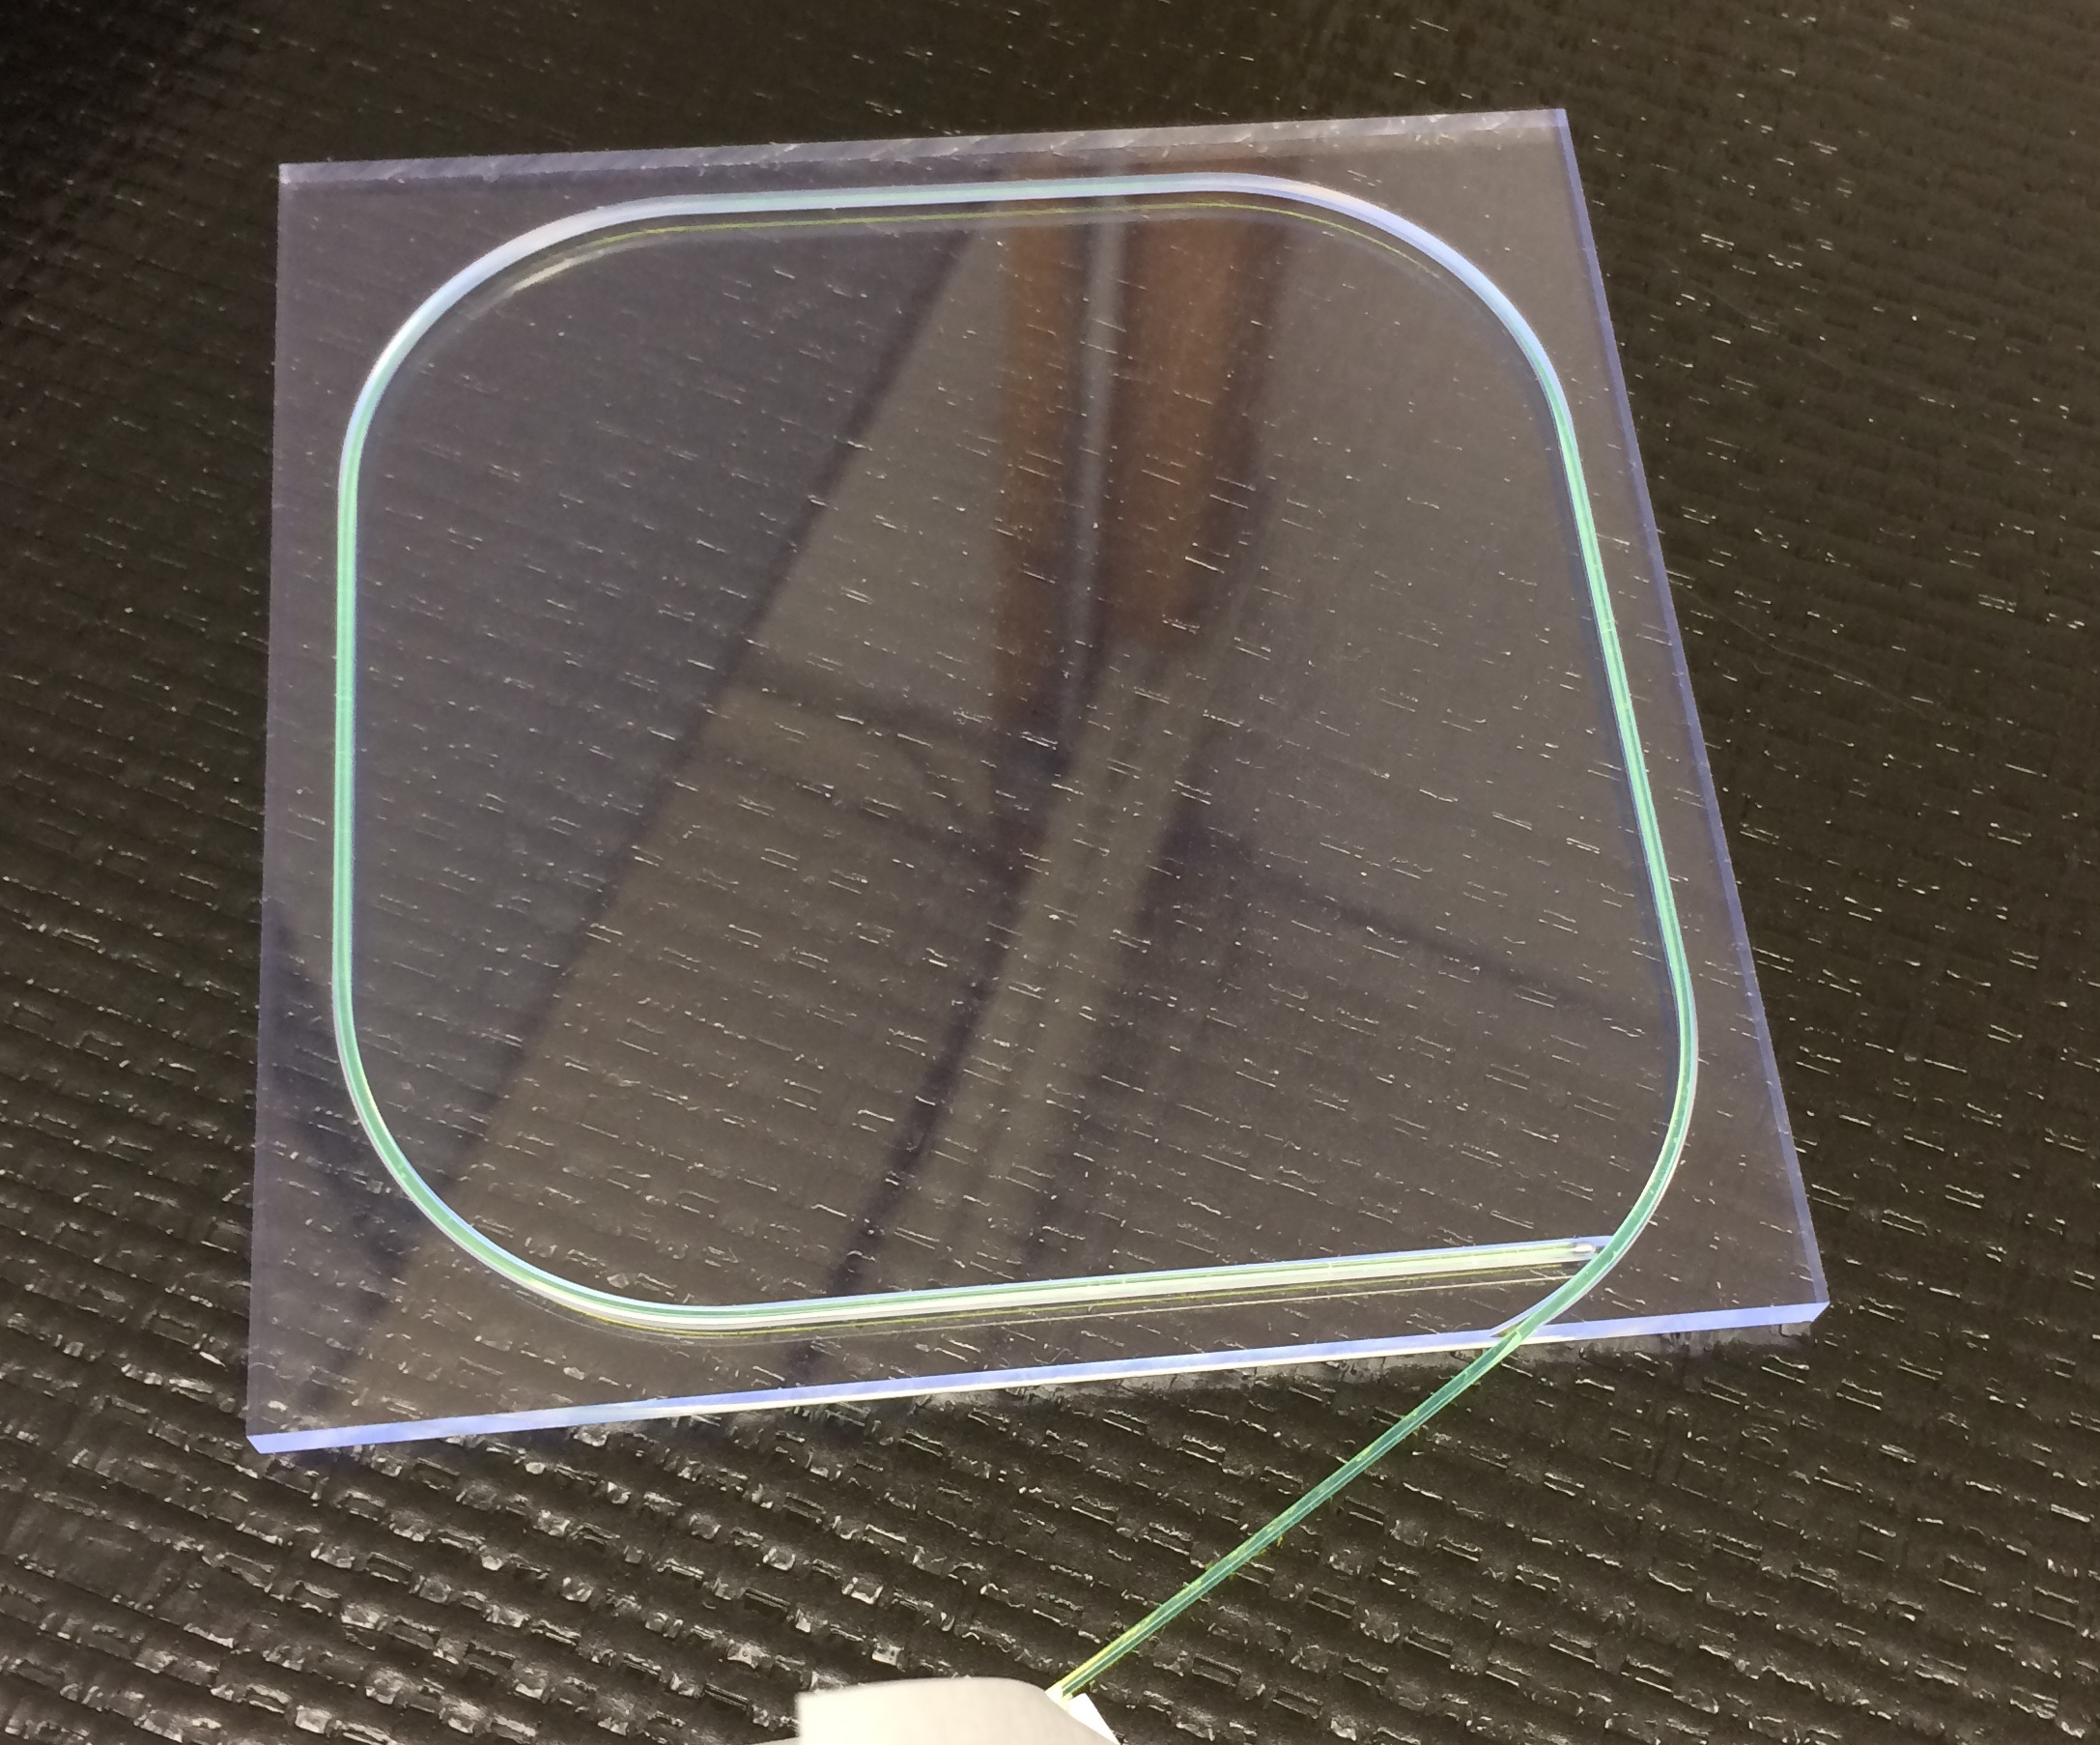
\includegraphics[width=0.4\textwidth]{figures/sigma}
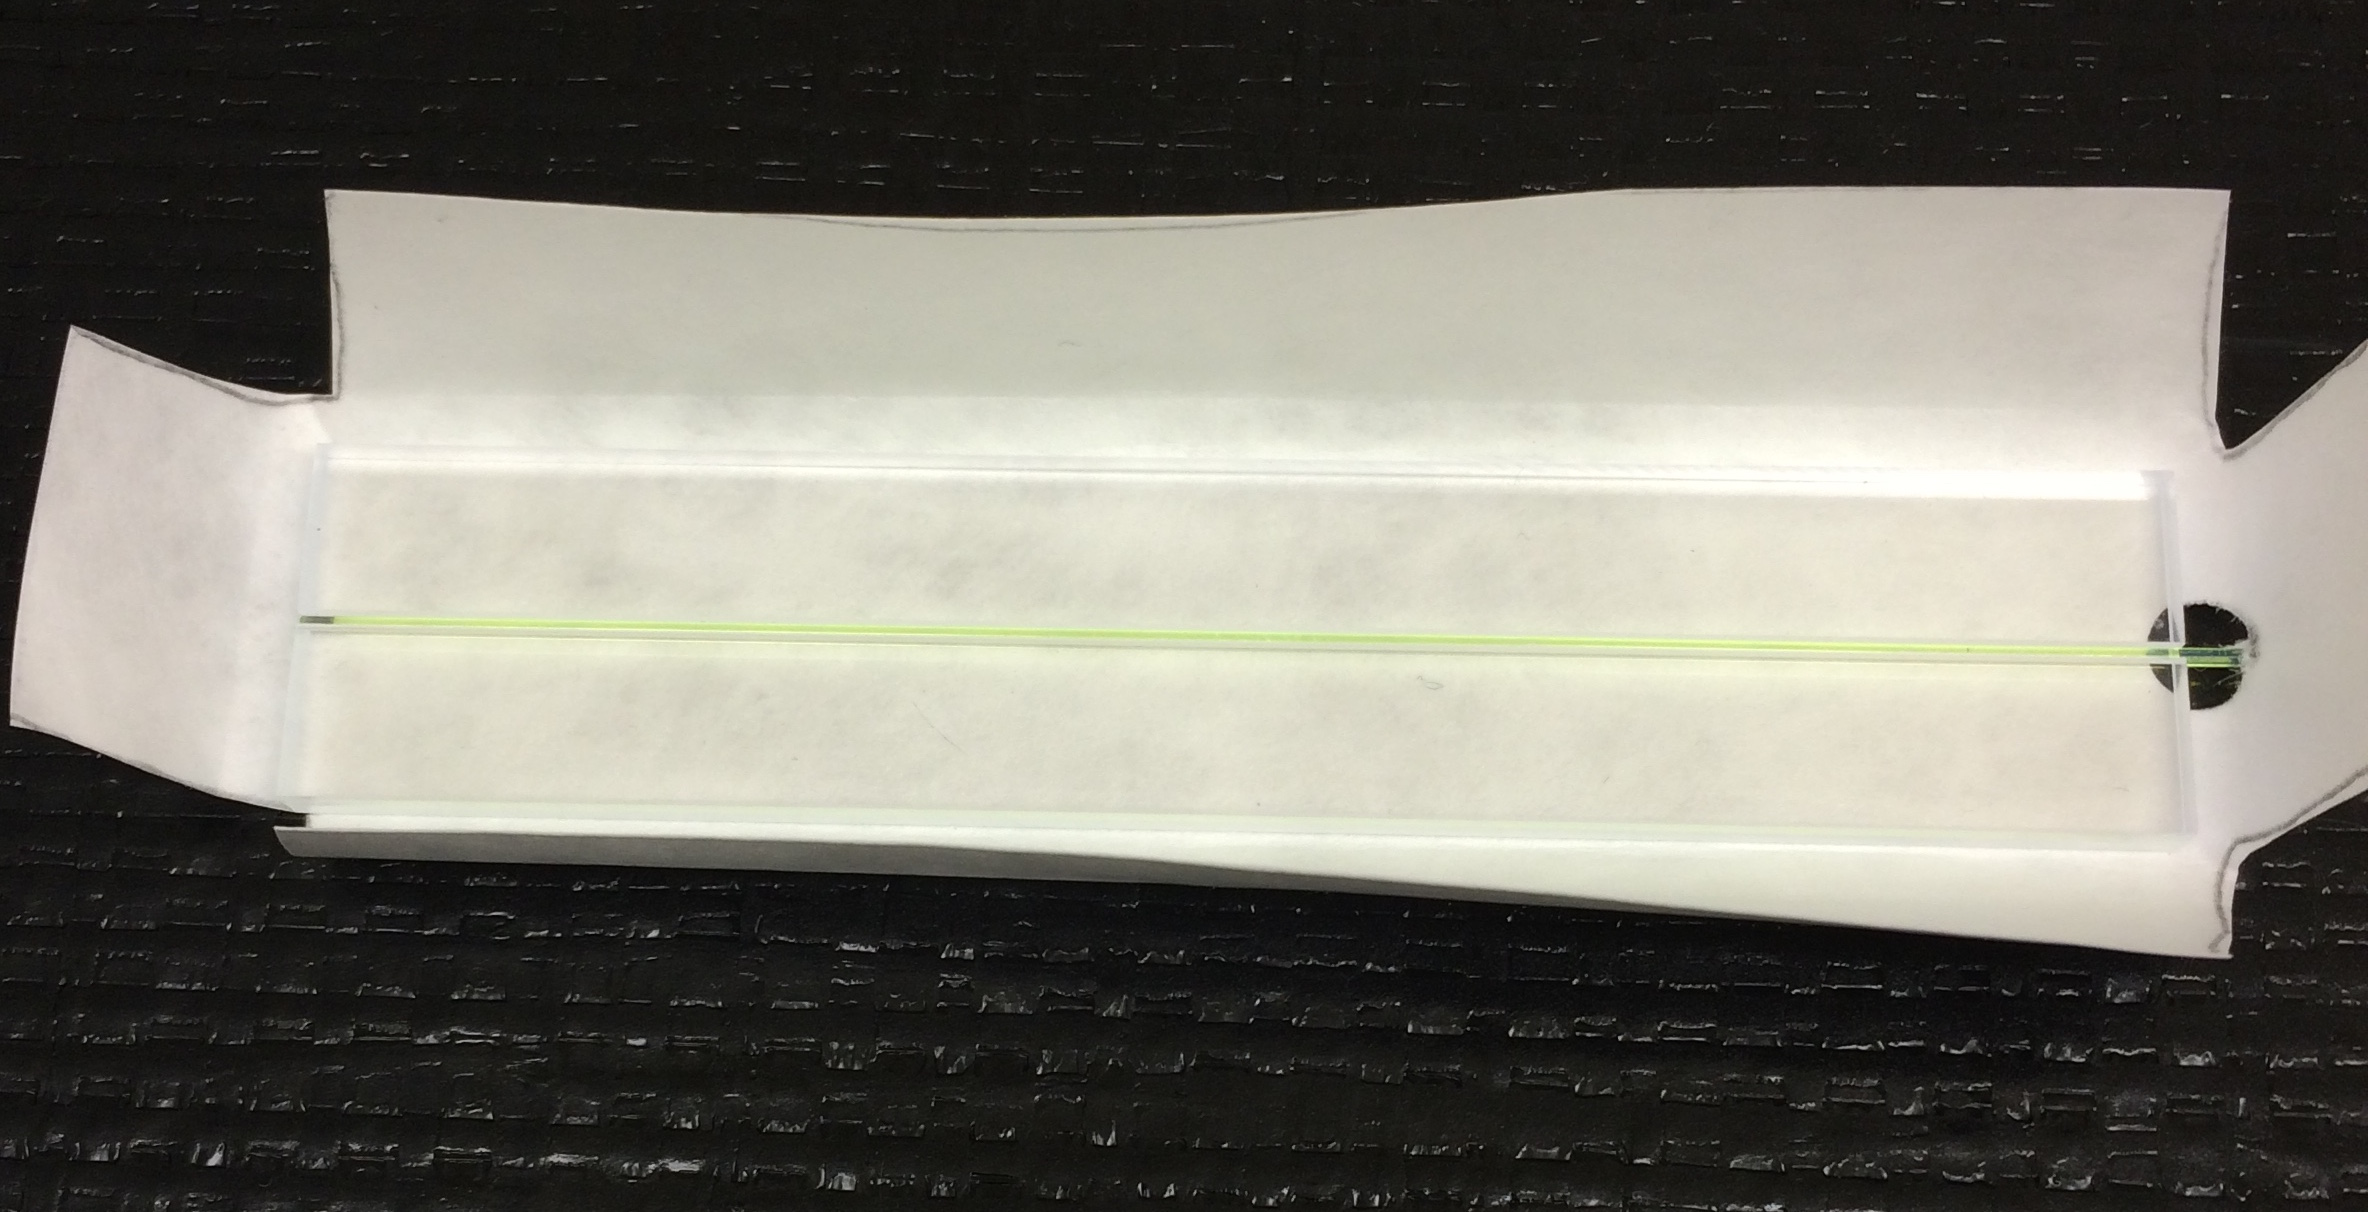
\includegraphics[width=0.4\textwidth]{figures/finger-horizontal}
\caption{(\cmsLeft) Sigma tile with green WLS fiber. (\cmsRight) Finger tile with green WLS fiber, lying on Tyvek wrapping.}
\label{fig:sigma-finger}
\end{center}
\end{figure}

In this experiment, there are two tiles with special geometries.
\begin{itemize}
\item \textbf{Multi-pronged sigma tile:} Two of the sigma tiles, instead of having a single WLS fiber with a sigma-shaped trajectory, have instead a number of straight, parallel WLS fibers running through them. Laser light is shined onto the tile above the center of each of the straight WLS fibers, as though they were finger tile WLS fibers. The signals from the fibers are read out separately by the readout system. One of these special tiles has four WLS fibers, with laser light fibers shining onto each of them. The other tile has three WLS fibers, two of which have a laser light fiber shining onto them, while the third does not and only receives scintillation light produced in the tile by the other two laser fibers that do not shine directly onto it. These two special sigma tile geometries will be referred to respectively as 4-pronged sigma tile and 3-pronged sigma tile.
\item \textbf{Truncated finger tile:} One of the finger tiles is only 5 cm long instead of 10 cm; all the other dimensions are normal.
\end{itemize}

The scintillator materials used in this study are:

\begin{table}[htbh]
\begin{center}
\topcaption{Properties of the scintillator materials analyzed for radiation tolerance on the CASTOR table: photons per 1-MeV electron, peak wavelength of emission, decay time, and base material. Some properties are not listed for Scintillator X because the material has not been patented yet. Guide to base material acronyms: PS = polystyrene. PVT = polyvinyltoluene. \label{tab:scint-materials}}
\begin{tabular}{|c|c|c|c|c|}
\hline
Material & $\gamma$/1MeV-$e$ yield & $\lambda_{em}$ (nm) & Decay time (ns) & Base material \\
\hline
\hline
SCSN81~\cite{Kuraray} &  & 430 & 2.5 & PS \\
EJ200~\cite{EJ200} & 10000 & 425 & 2.1 & PVT \\
EJ260~\cite{EJ260} & 9200 & 490 & 9.2 & PVT \\
Scintillator X &  &  &  &  \\
LS6946 &  &  &  & Polysiloxane \\
PTP &  &  &  &  \\
PEN &  &  &  &  \\
PET &  &  &  &  \\
\hline
\end{tabular}
\end{center}
\end{table}

\begin{table}[htbh]
\begin{center}
\topcaption{Properties of the wavelength-shifters (WLS) used in this experiment: material type, the tiles they were used with, peak wavelength of absorption, peak wavelength of emission, and diameter. The second column lists the types of scintillator material (see Table~\ref{tab:scint-materials}) that each WLS was used with. All WLS fibers were multi-cladded, with numerical aperture 0.72, trapping efficiency 5.4\%, and cladding thickness equal to 4\% of their diameter~\cite{KuraWLS}.\label{tab:WLS-materials}}
\begin{tabular}{|c|c|c|c|c|}
\hline
Material & Used with tile(s) & $\lambda_{abs}$ (nm) & $\lambda_{em}$ (nm) & Diameter (mm) \\
\hline
Y11~\cite{KuraWLS} & SCSN81, EJ200, Scint. X, PEN & 430 & 476 & 0.94 \\
O2~\cite{KuraWLS} & EJ260 & 535 & 550 & 0.98 \\
B2~\cite{KuraWLS} & PTP, PET & 375 & 437 & 0.98 \\
\hline
\end{tabular}
\end{center}
\end{table}

The scintillator samples are wrapped individually in reflective Tyvek material and stored inside black plastic cassettes to isolate them from external light. One cassette can hold either one sigma tile or up to four finger tiles. Figures~\ref{fig:sigmatile}-~\ref{fig:fingertile} show how wrapped sigma tiles and finger tiles are arranged inside their cassettes. There are a few tiles with exceptional shapes: Scintillator X (Figure~\ref{fig:scintXtile}) has a truncated finger geometry, and PTP (Figure~\ref{fig:PTPtile}) and PEN (Figure~\ref{fig:PENtile}) have 4-pronged and 3-pronged sigma tile geometries respectively; the third WLS fiber in the PEN tile does not have a laser fiber shining onto it.

\begin{figure}[hbtp]
\begin{center}
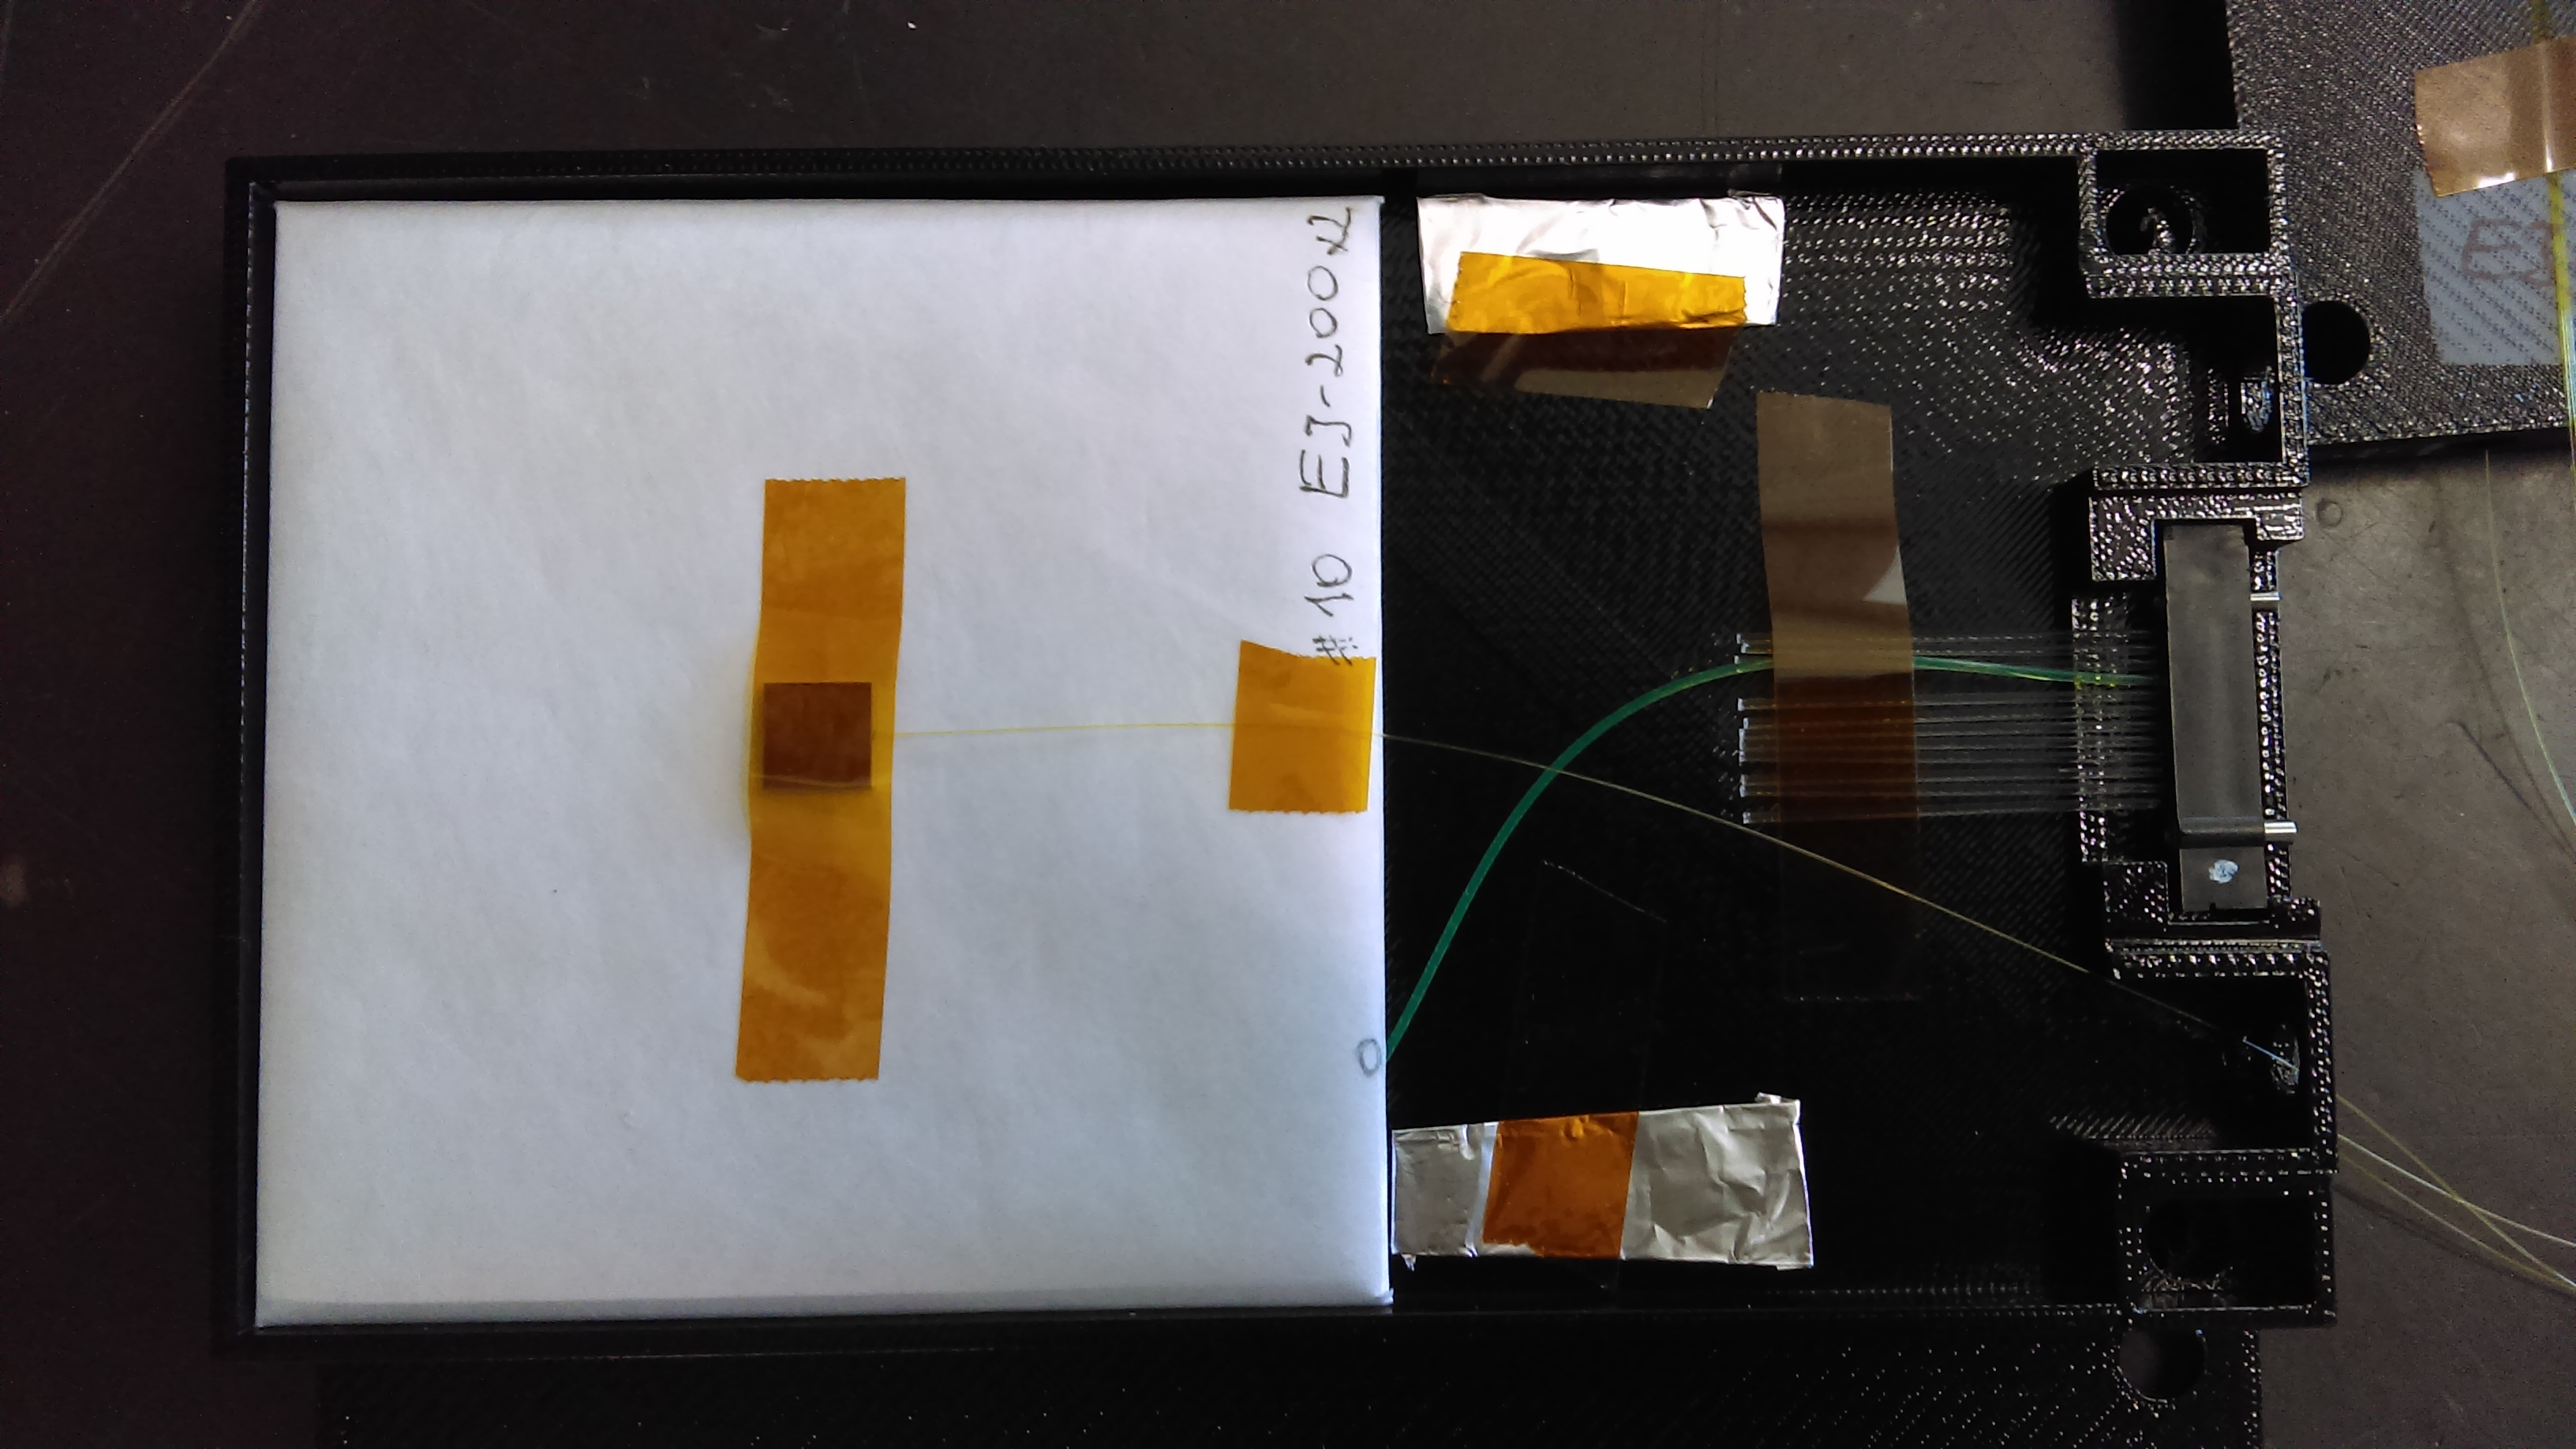
\includegraphics[width=0.75\textwidth]{figures/sigmatile}
\caption{EJ200 sigma tile inside a cassette.}
\label{fig:sigmatile}
\end{center}
\end{figure}

\begin{figure}[hbtp]
\begin{center}
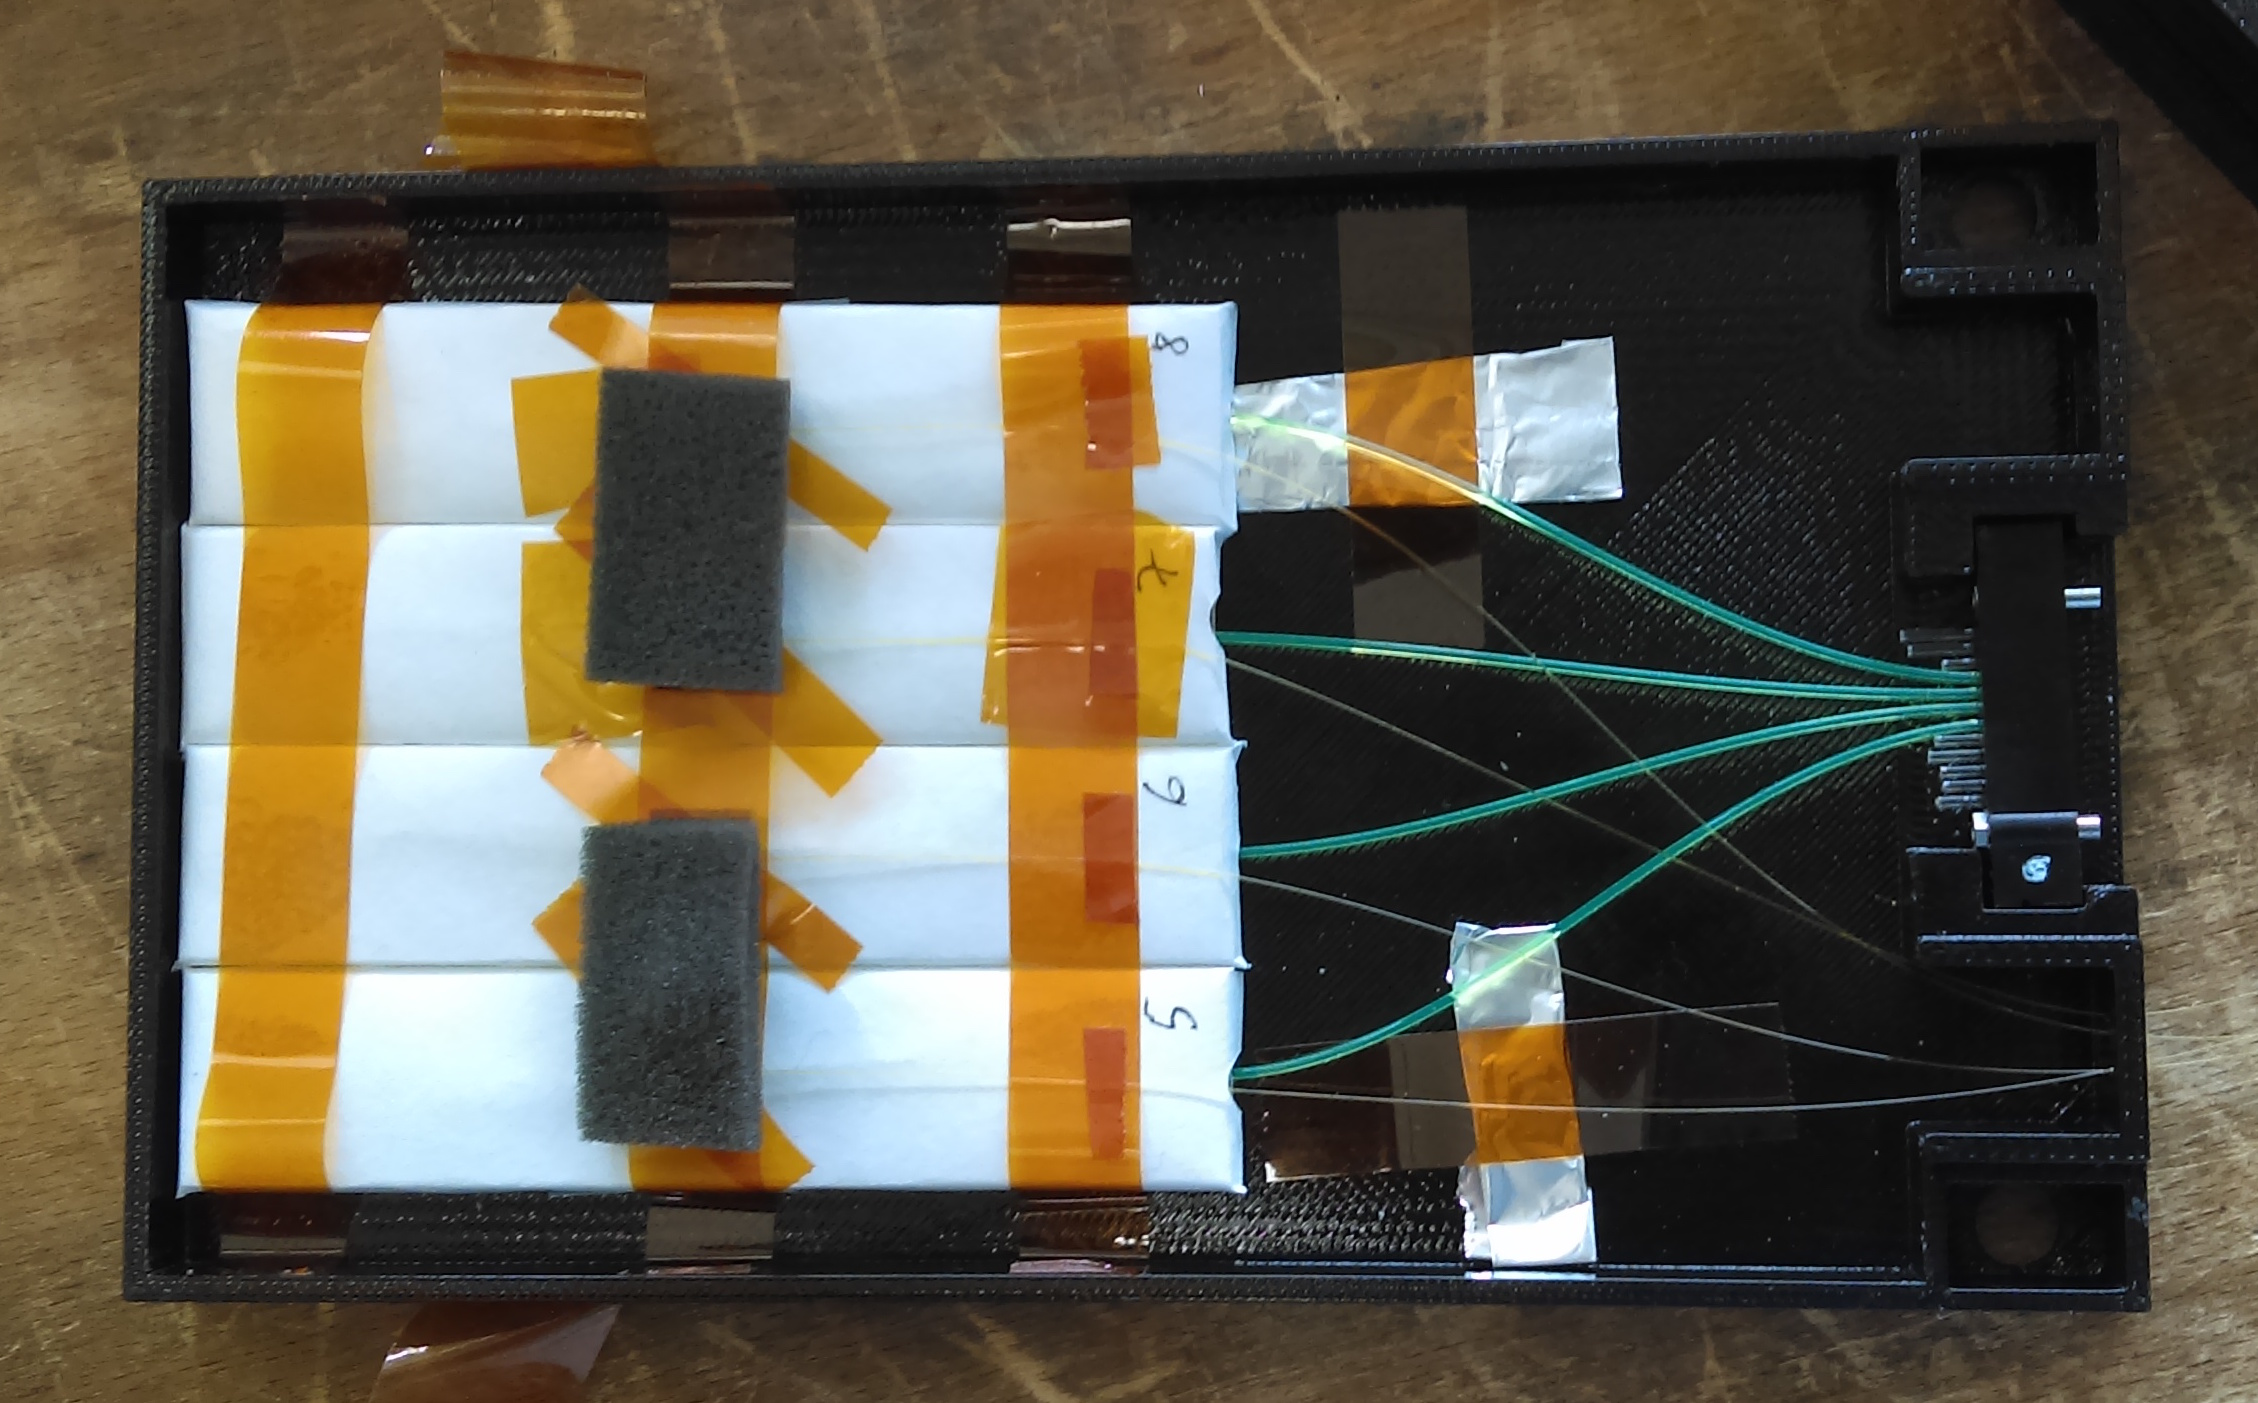
\includegraphics[width=0.75\textwidth]{figures/fingertile}
\caption{SCSN-81 finger tiles inside a cassette.}
\label{fig:fingertile}
\end{center}
\end{figure}

\begin{figure}[hbtp]
\begin{center}
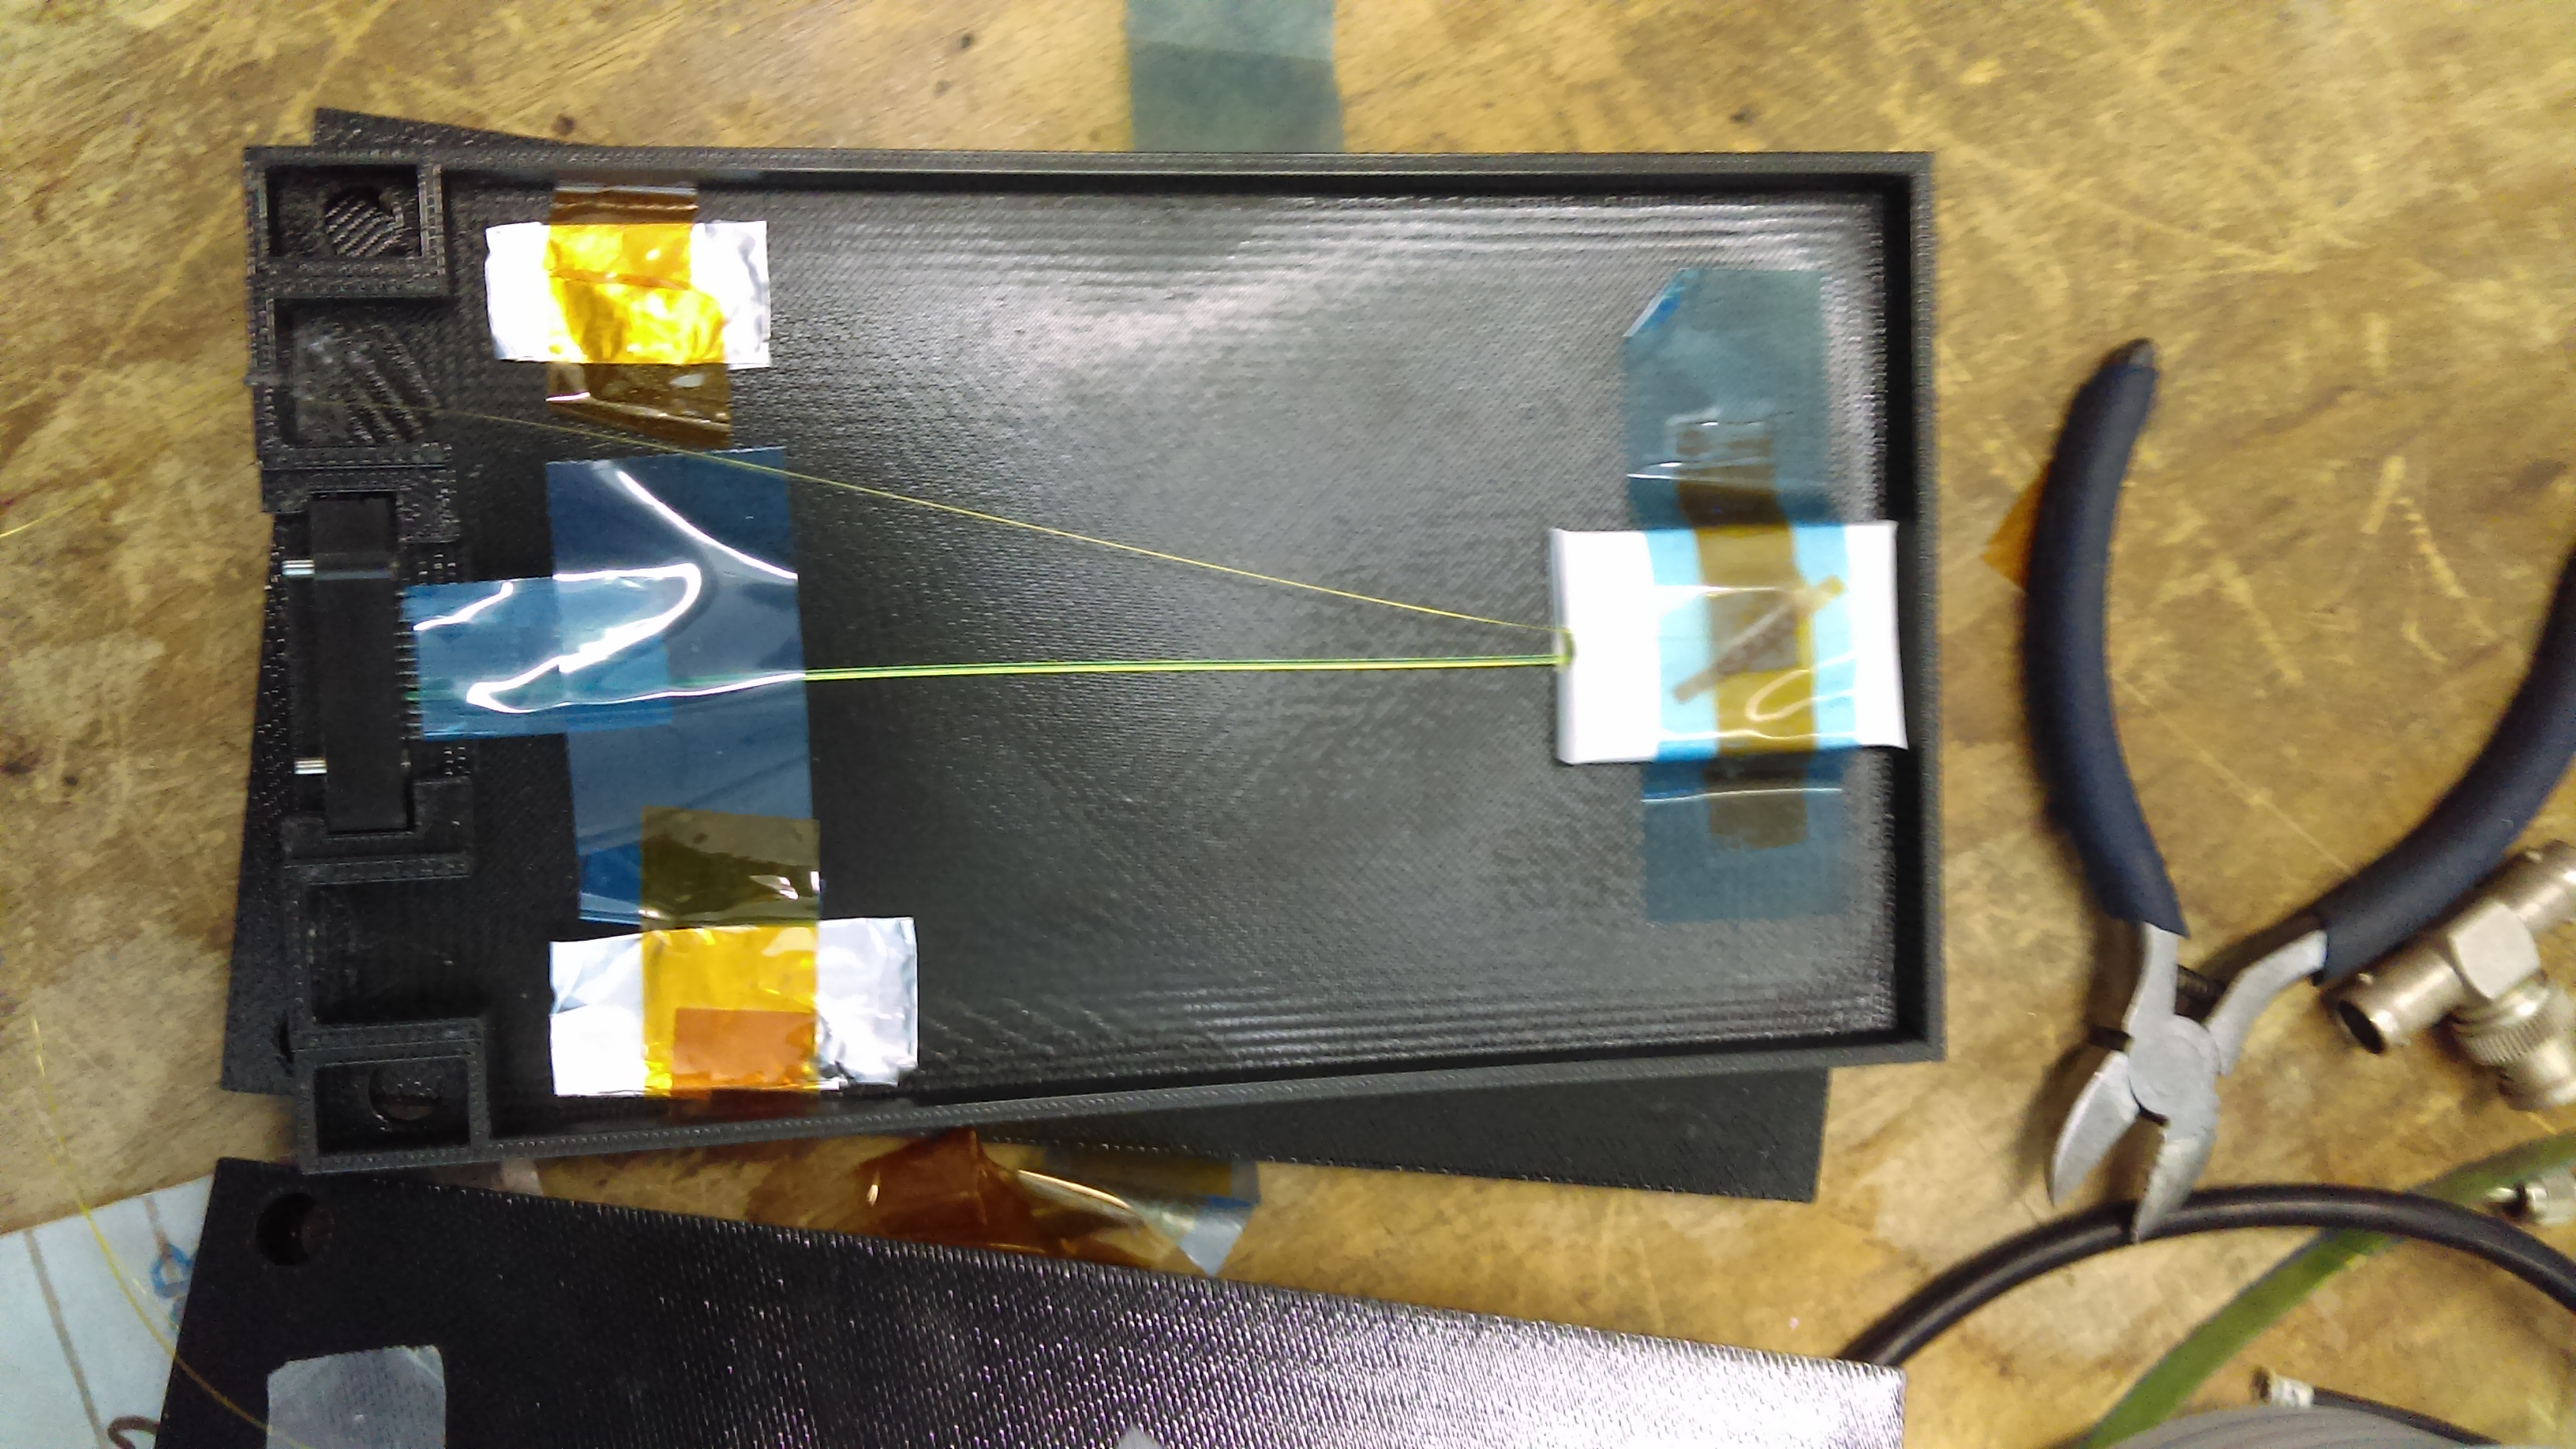
\includegraphics[width=0.75\textwidth]{figures/scintXtile}
\caption{Scintillator X truncated finger tile inside a cassette.}
\label{fig:scintXtile}
\end{center}
\end{figure}

\begin{figure}[hbtp]
\begin{center}
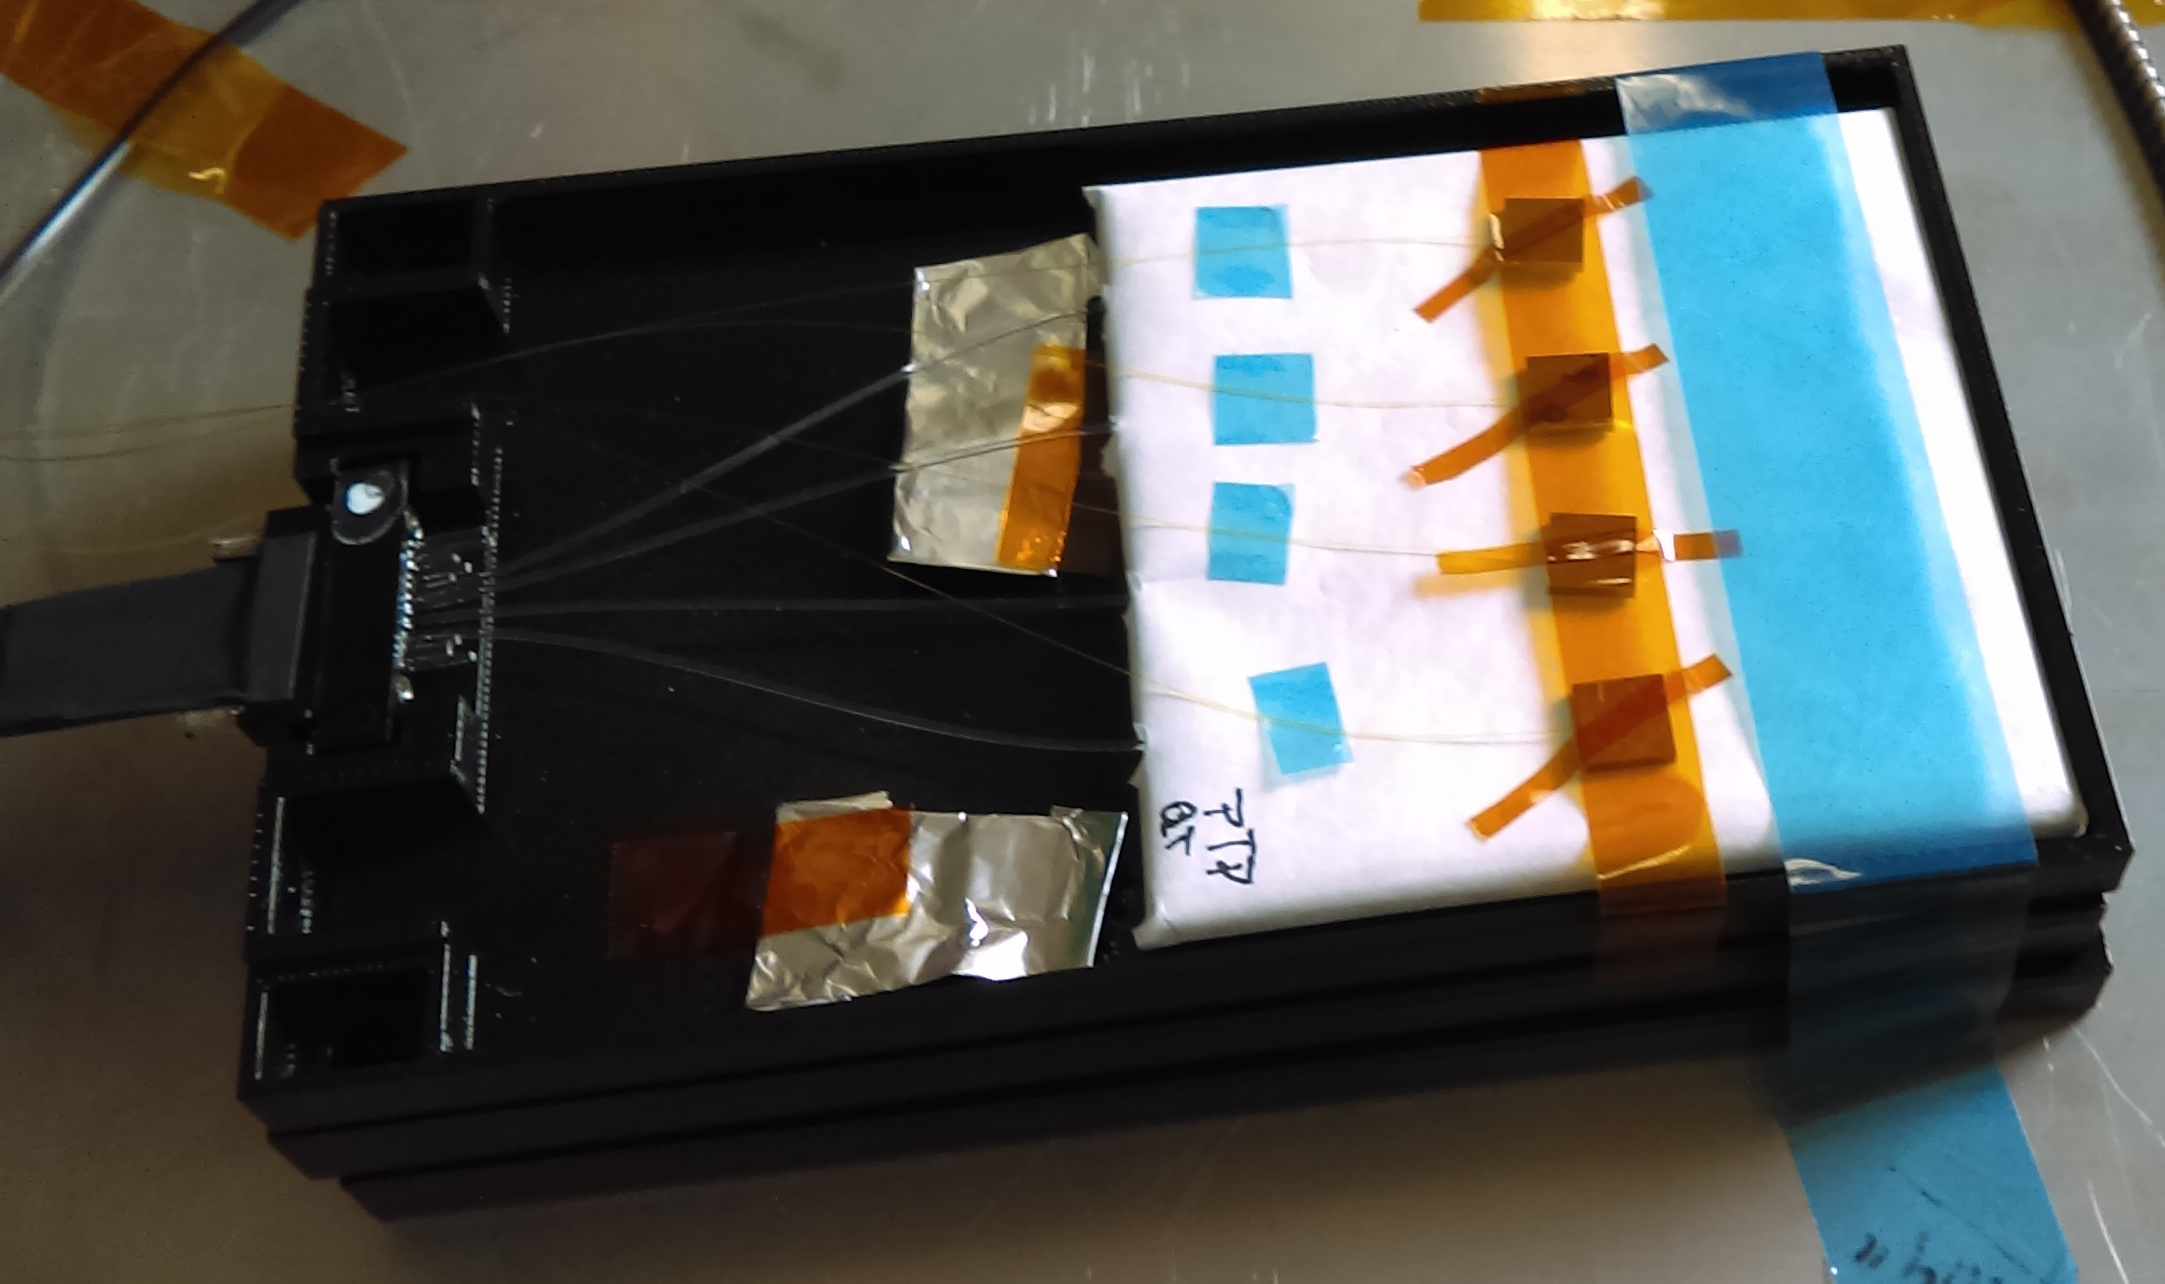
\includegraphics[width=0.75\textwidth]{figures/PTPtile}
\caption{PTP 4-pronged sigma tile inside a cassette.}
\label{fig:PTPtile}
\end{center}
\end{figure}

\begin{figure}[hbtp]
\begin{center}
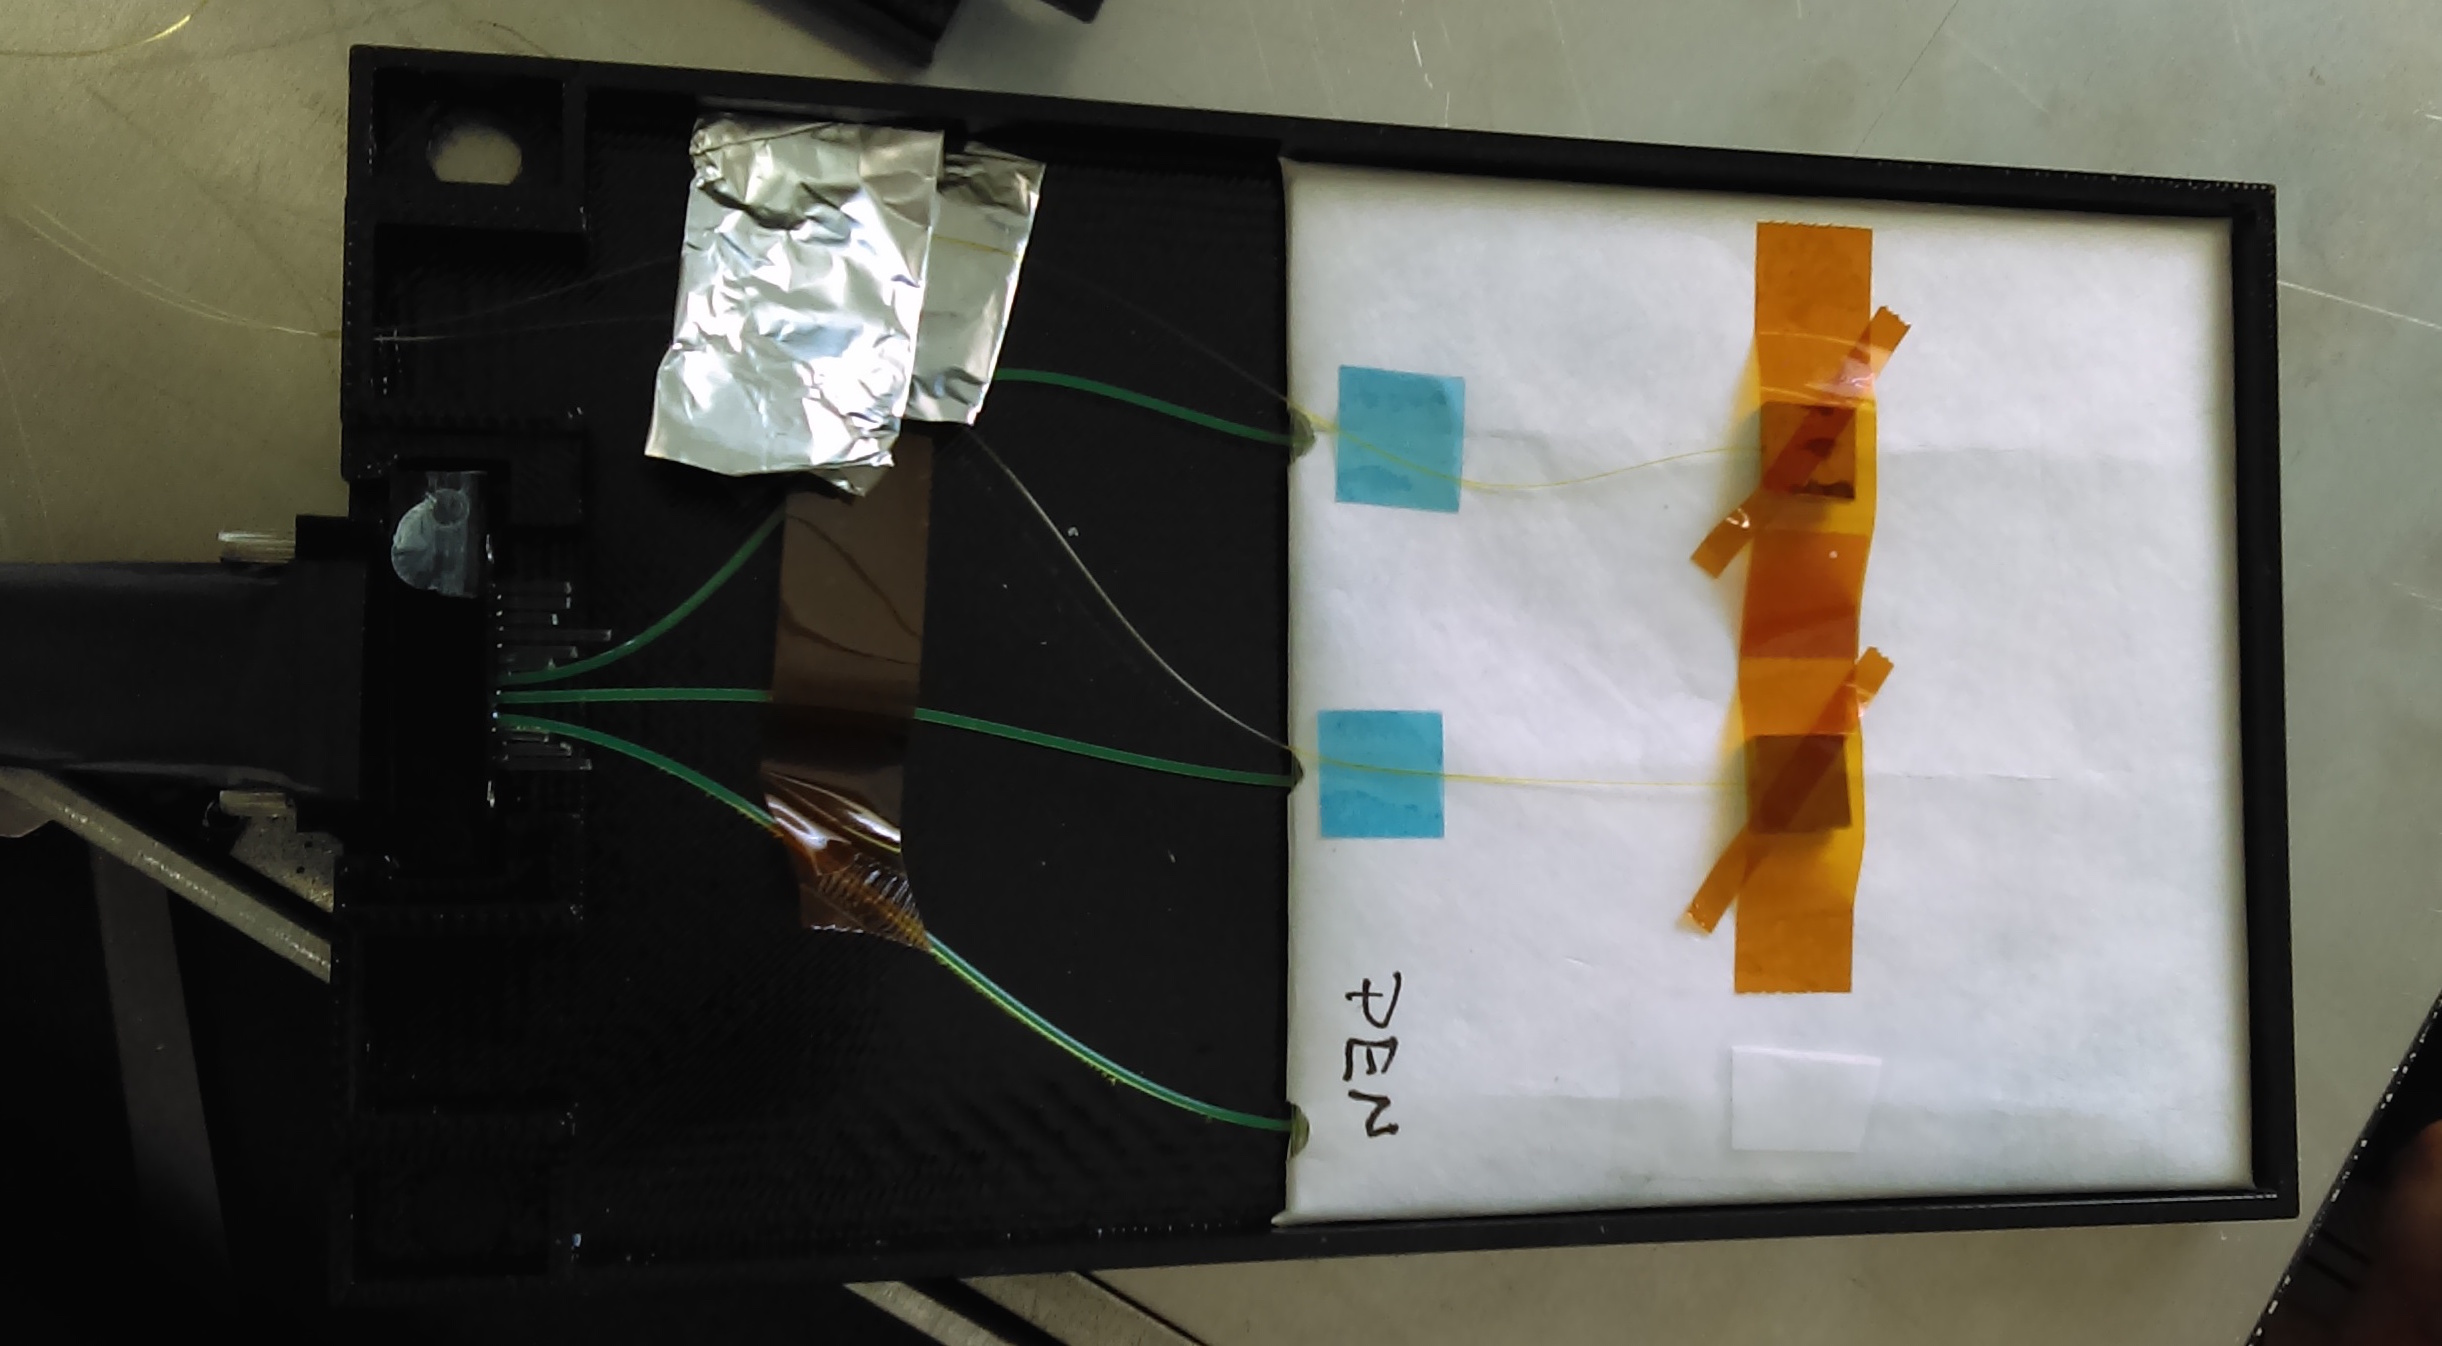
\includegraphics[width=0.75\textwidth]{figures/PENtile}
\caption{PEN 3-pronged sigma tile inside a cassette. One of the WLS fibers was intentionally left without a laser fiber illuminating it.}
\label{fig:PENtile}
\end{center}
\end{figure}

\subsection{Dark Boxes\label{sec:setup-darkboxes}}

The scintillator samples inside their cassettes are to be placed on the CRF platform to be irradiated close the LHC beam-pipe, at an expected dose rate of $\mathcal{O}$(1-10) krad/hr, depending on the distance from the beampipe. Two ``Dark Boxes" with dimensions 39.9 cm $\times$ 34.8 cm $\times$ 18.1 cm have been designed and built by Fermilab to hold the cassettes. Each box can hold 24 cassettes and also contains a laser light injection box that splits uniformly the incoming laser light among the cassettes, a system of plastic tubes for circulating dry air through the cassettes to keep the environmental humidity low, and a system of clear fibers that carry scintillation light from individual tiles.

Light of wavelength 351 nm from the USC laser source at Point 5 is used to illuminate the scintillators. The laser light reaching the light injection box is split between nine identical outputs. To each of these outputs is connected a bundle of CeramOptec quartz core-fibers with core cladding (core diameter 250 $\mu$m and total diameter 280 $\mu$m including cladding). From these bundles, one or more laser fibers enter each cassette to illuminate the scintillator sample(s) within. Inside the cassette, each laser fiber terminates at a metallic mirror that directs the light onto a dedicated scintillator sample through a hole in the Tyvek covering; the hole is small enough that the metallic mirror, lying directly on top of it, blocks any other light from entering except the light from the laser fiber. The scintillation light produced in each tile is collected by a WLS fiber (see Table~\ref{tab:WLS-materials} for the materials and dimensions of the various WLS fibers used) which is spliced to a 0.94 mm-diameter, multi-cladded clear fiber~\cite{KuraWLS} as it exits the cassette.

Inside the Dark Box, the cassettes are arranged in stacks of 6 or 9. When the Dark Box is placed under the beam pipe, the cassette stacks are all located directly below the beampipe at the same azimuthal ($\phi$) position, and thus the distances of the various tiles from the beam axis differ only in the radial dimension r. Tables~\ref{tab:distances-box1} and~\ref{tab:distances-box2} list the distances, in Dark Boxes 1 and 2 respectively, of each scintillator material sample from the beampipe.

\begin{table}
\begin{center}
\begin{tabular}{|c|c|c|}
\hline
Material & Shapes & Distance (cm) \\
\hline
\multirow{9}{*}{SCSN81} & 1S & 11.8 \\
& 1S & 13.1 \\
& 4F & 14.4 \\
& 1S & 18.2 \\
& 1S & 19.5 \\
& 4F & 20.8 \\
& 2S & 24.6 \\
& 2S & 25.9 \\
& 6F & 27.2 \\
\hline
\multirow{2}{*}{EJ200} & 1S & 13.1 \\
& 1S & 19.5 \\
\hline
\multirow{7}{*}{EJ260} & 2S & 11.8 \\
& 1S & 13.1 \\
& 4F & 14.4 \\
& 1S & 18.2 \\
& 2F & 20.8 \\
& 1S & 24.6 \\
& 2F & 27.2 \\
\hline
\end{tabular}
\caption{Table of scintillator samples in Dark Box 1 and their respective distances from the beamline in cm. The first column lists the material type. The second column lists the number of tiles with sigma (S) and finger (F) shapes; for example, an entry of "4F" means that there are four finger tiles at this radius from the beamline. The third column lists the distance from the beamline. The uncertainty of the distance measurements is conservatively estimated to be +/-1 cm.}
\label{tab:distances-box1}
\end{center}
\end{table}

\begin{table}
\begin{center}
\begin{tabular}{|c|c|c|}
\hline
Material & Shapes & Distance (cm) \\
\hline
\multirow{9}{*}{SCSN81} & 1S & 11.8 \\
& 1S & 13.1 \\
& 4F & 14.4 \\
& 2S & 18.2 \\
& 2S & 19.5 \\
& 4F & 20.8 \\
& 3S & 24.6 \\
& 2S & 25.9 \\
& 4F & 27.2 \\
\hline
\multirow{4}{*}{EJ200} & 1S & 11.8 \\
& 1S & 13.1 \\
& 1S & 19.5 \\
& 1S & 25.9 \\
\hline
PTP & 1S(4-prong) & 11.8 \\
\hline
PEN & 1S(3-prong) & 13.1 \\
\hline
PET & 1S & 14.4 \\
\hline
Scintillator X & 1F(truncated) & 13.1 \\
\hline
LS6946 & 2F & 27.2 \\
\hline
\end{tabular}
\caption{Table of scintillator samples in Dark Box 2 and their respective distances from the beamline in cm. The first column lists the material type. The second column lists the number of tiles with sigma (S) and finger (F) shapes; for example, an entry of "4F" means that there are four finger tiles at this radius from the beamline. The third column lists the distance from the beamline. The uncertainty of the distance measurements is conservatively estimated to be +/-1 cm. N.B.: scintillator X, PTP, and PEN all have special tile geometries, described in Sec.~\ref{sec:setup-tiles}.}
\label{tab:distances-box2}
\end{center}
\end{table}

Figure~\ref{fig:box-schematic} shows the arrangement of the cassette stacks inside Dark Boxes 1 and 2; the material of each scintillator sample is indicated, as well as its shape (``S" at the end of the name stands for sigma tile, and ``F" stands for finger tile). Figures~\ref{fig:dark-box-1} and~\ref{fig:dark-box-2} show exterior and interior views respectively of a Dark Box.

\begin{figure}[hbtp]
\begin{center}
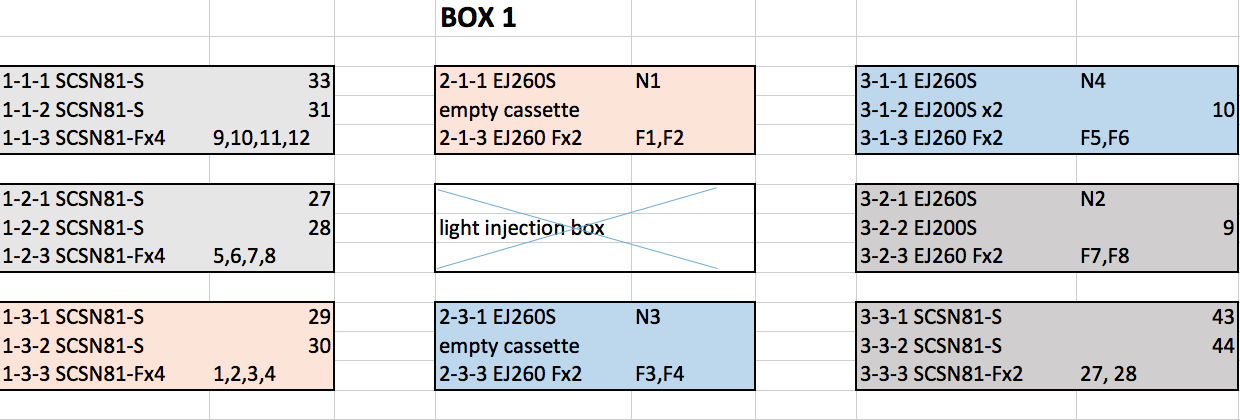
\includegraphics[width=0.8\textwidth]{figures/Box1_SamplesMap}
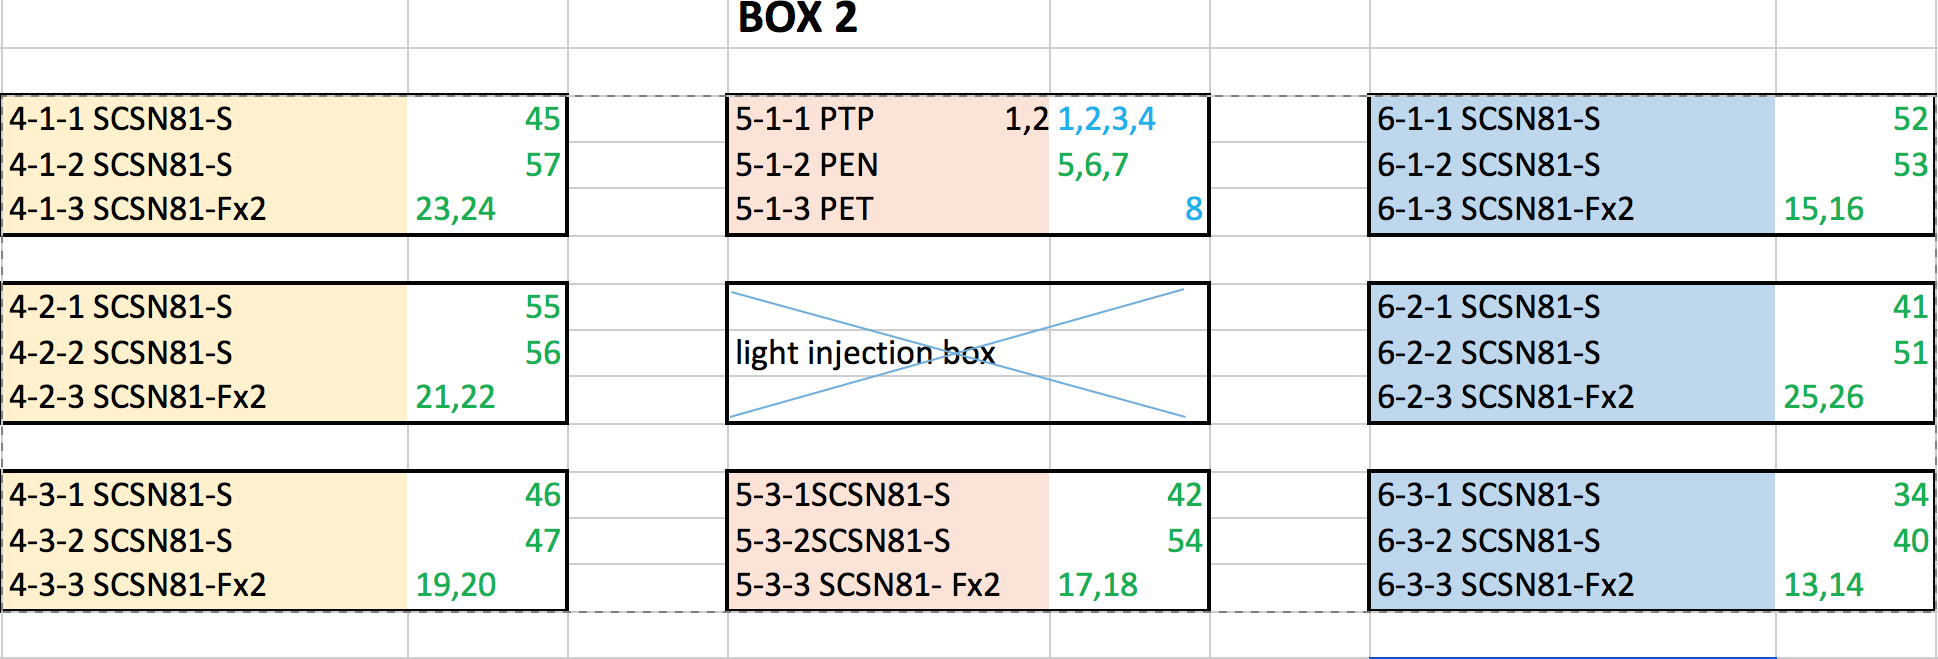
\includegraphics[width=0.8\textwidth]{figures/Box2_SamplesMap}
\caption{(Top) Arrangement of cassettes inside Dark Box 1. (Bottom) Arrangement of cassettes inside Dark Box 2. In these diagrams, the numbered labels ``X-Y-Z" on the left-hand side of each stack identify the cassette positions inside the box. The numbers at the right-hand side of each stack are used to connect the cassettes correctly to the clear fibers that carry the scintillation light out of the Dark Box. When the Dark Boxes are on the CASTOR table, the beam pipe (z-axis) runs from left to right across the top of each figure, meaning that cassettes numbered ``X-1-1" are closest to the beampipe and that those numbered ``X-3-3" are farthest from the beampipe. All cassettes in the same row are at the same distance from the beampipe.}
\label{fig:box-schematic}
\end{center}
\end{figure}

\begin{figure}[hbtp]
\begin{center}
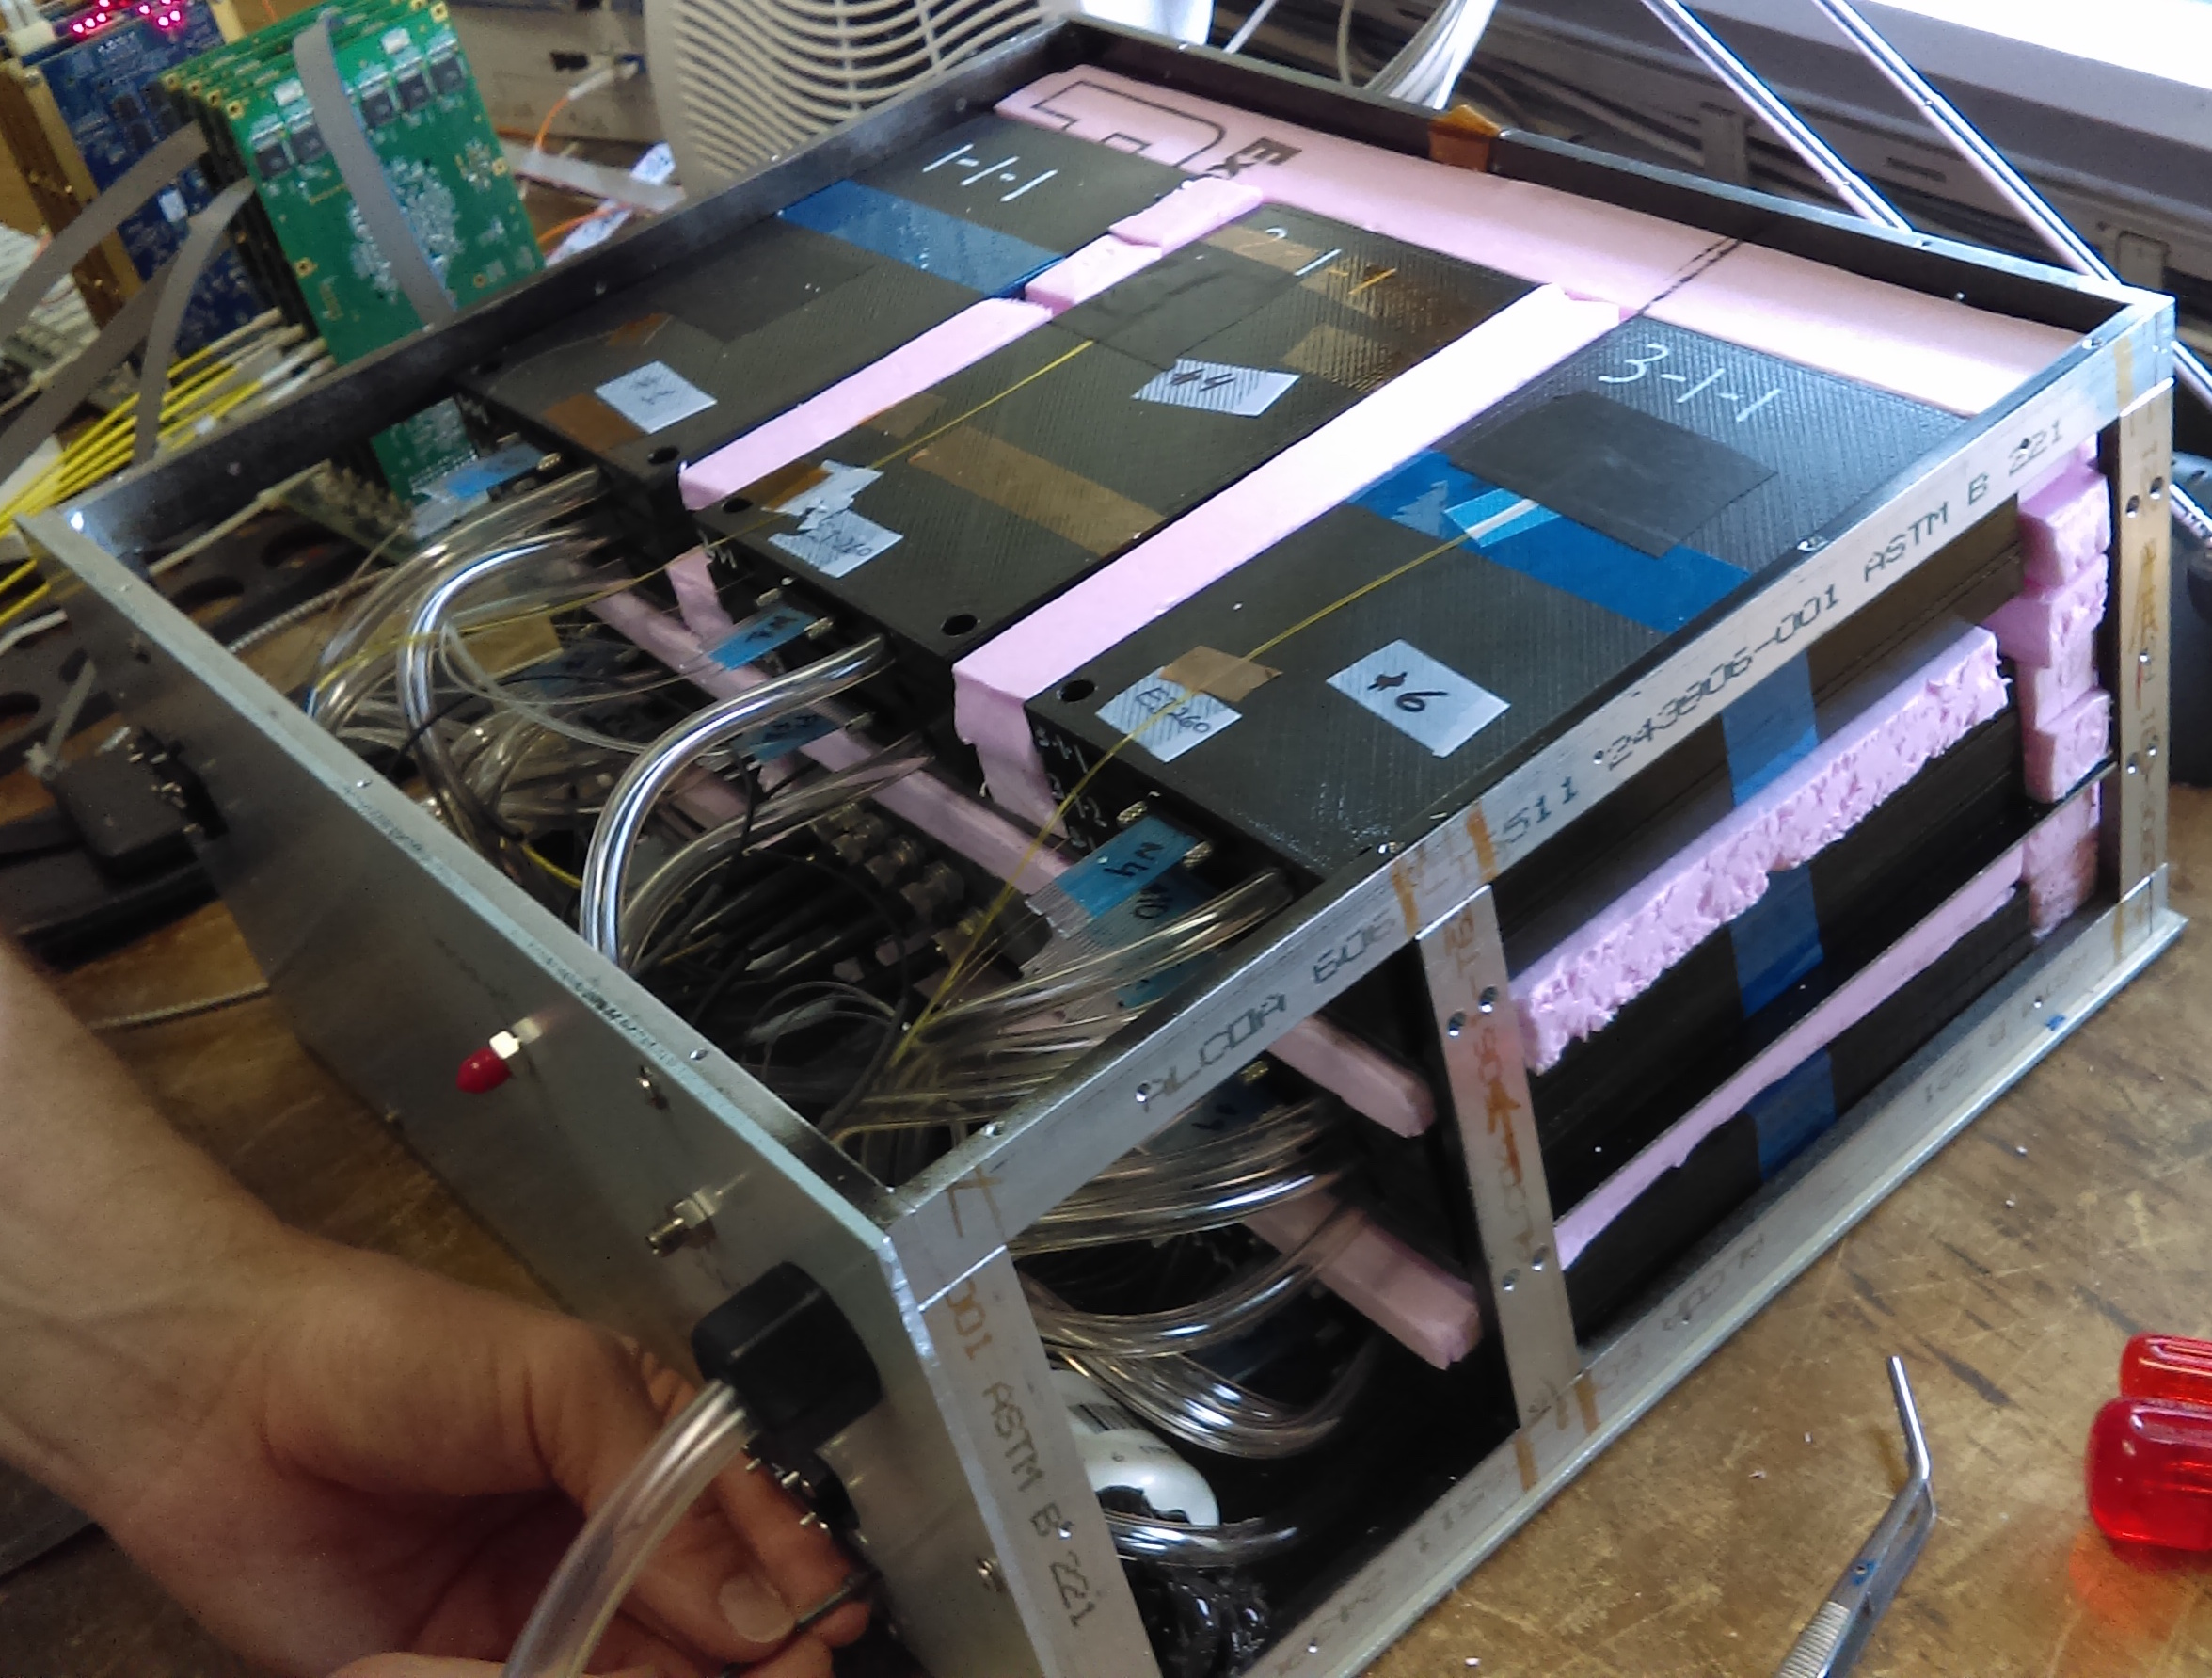
\includegraphics[width=0.8\textwidth]{figures/dark-box-1}
\caption{Photo of a partially disassembled Dark Box with some of the walls removed. Inside the Dark Box are: an array of 24 scintillator cassettes (black plastic boxes), a laser splitter box, cables of clear fibers, a dry air distribution system, and pieces of styrofoam that hold the cassettes in position.}
\label{fig:dark-box-1}
\end{center}
\end{figure}

\begin{figure}[hbtp]
\begin{center}
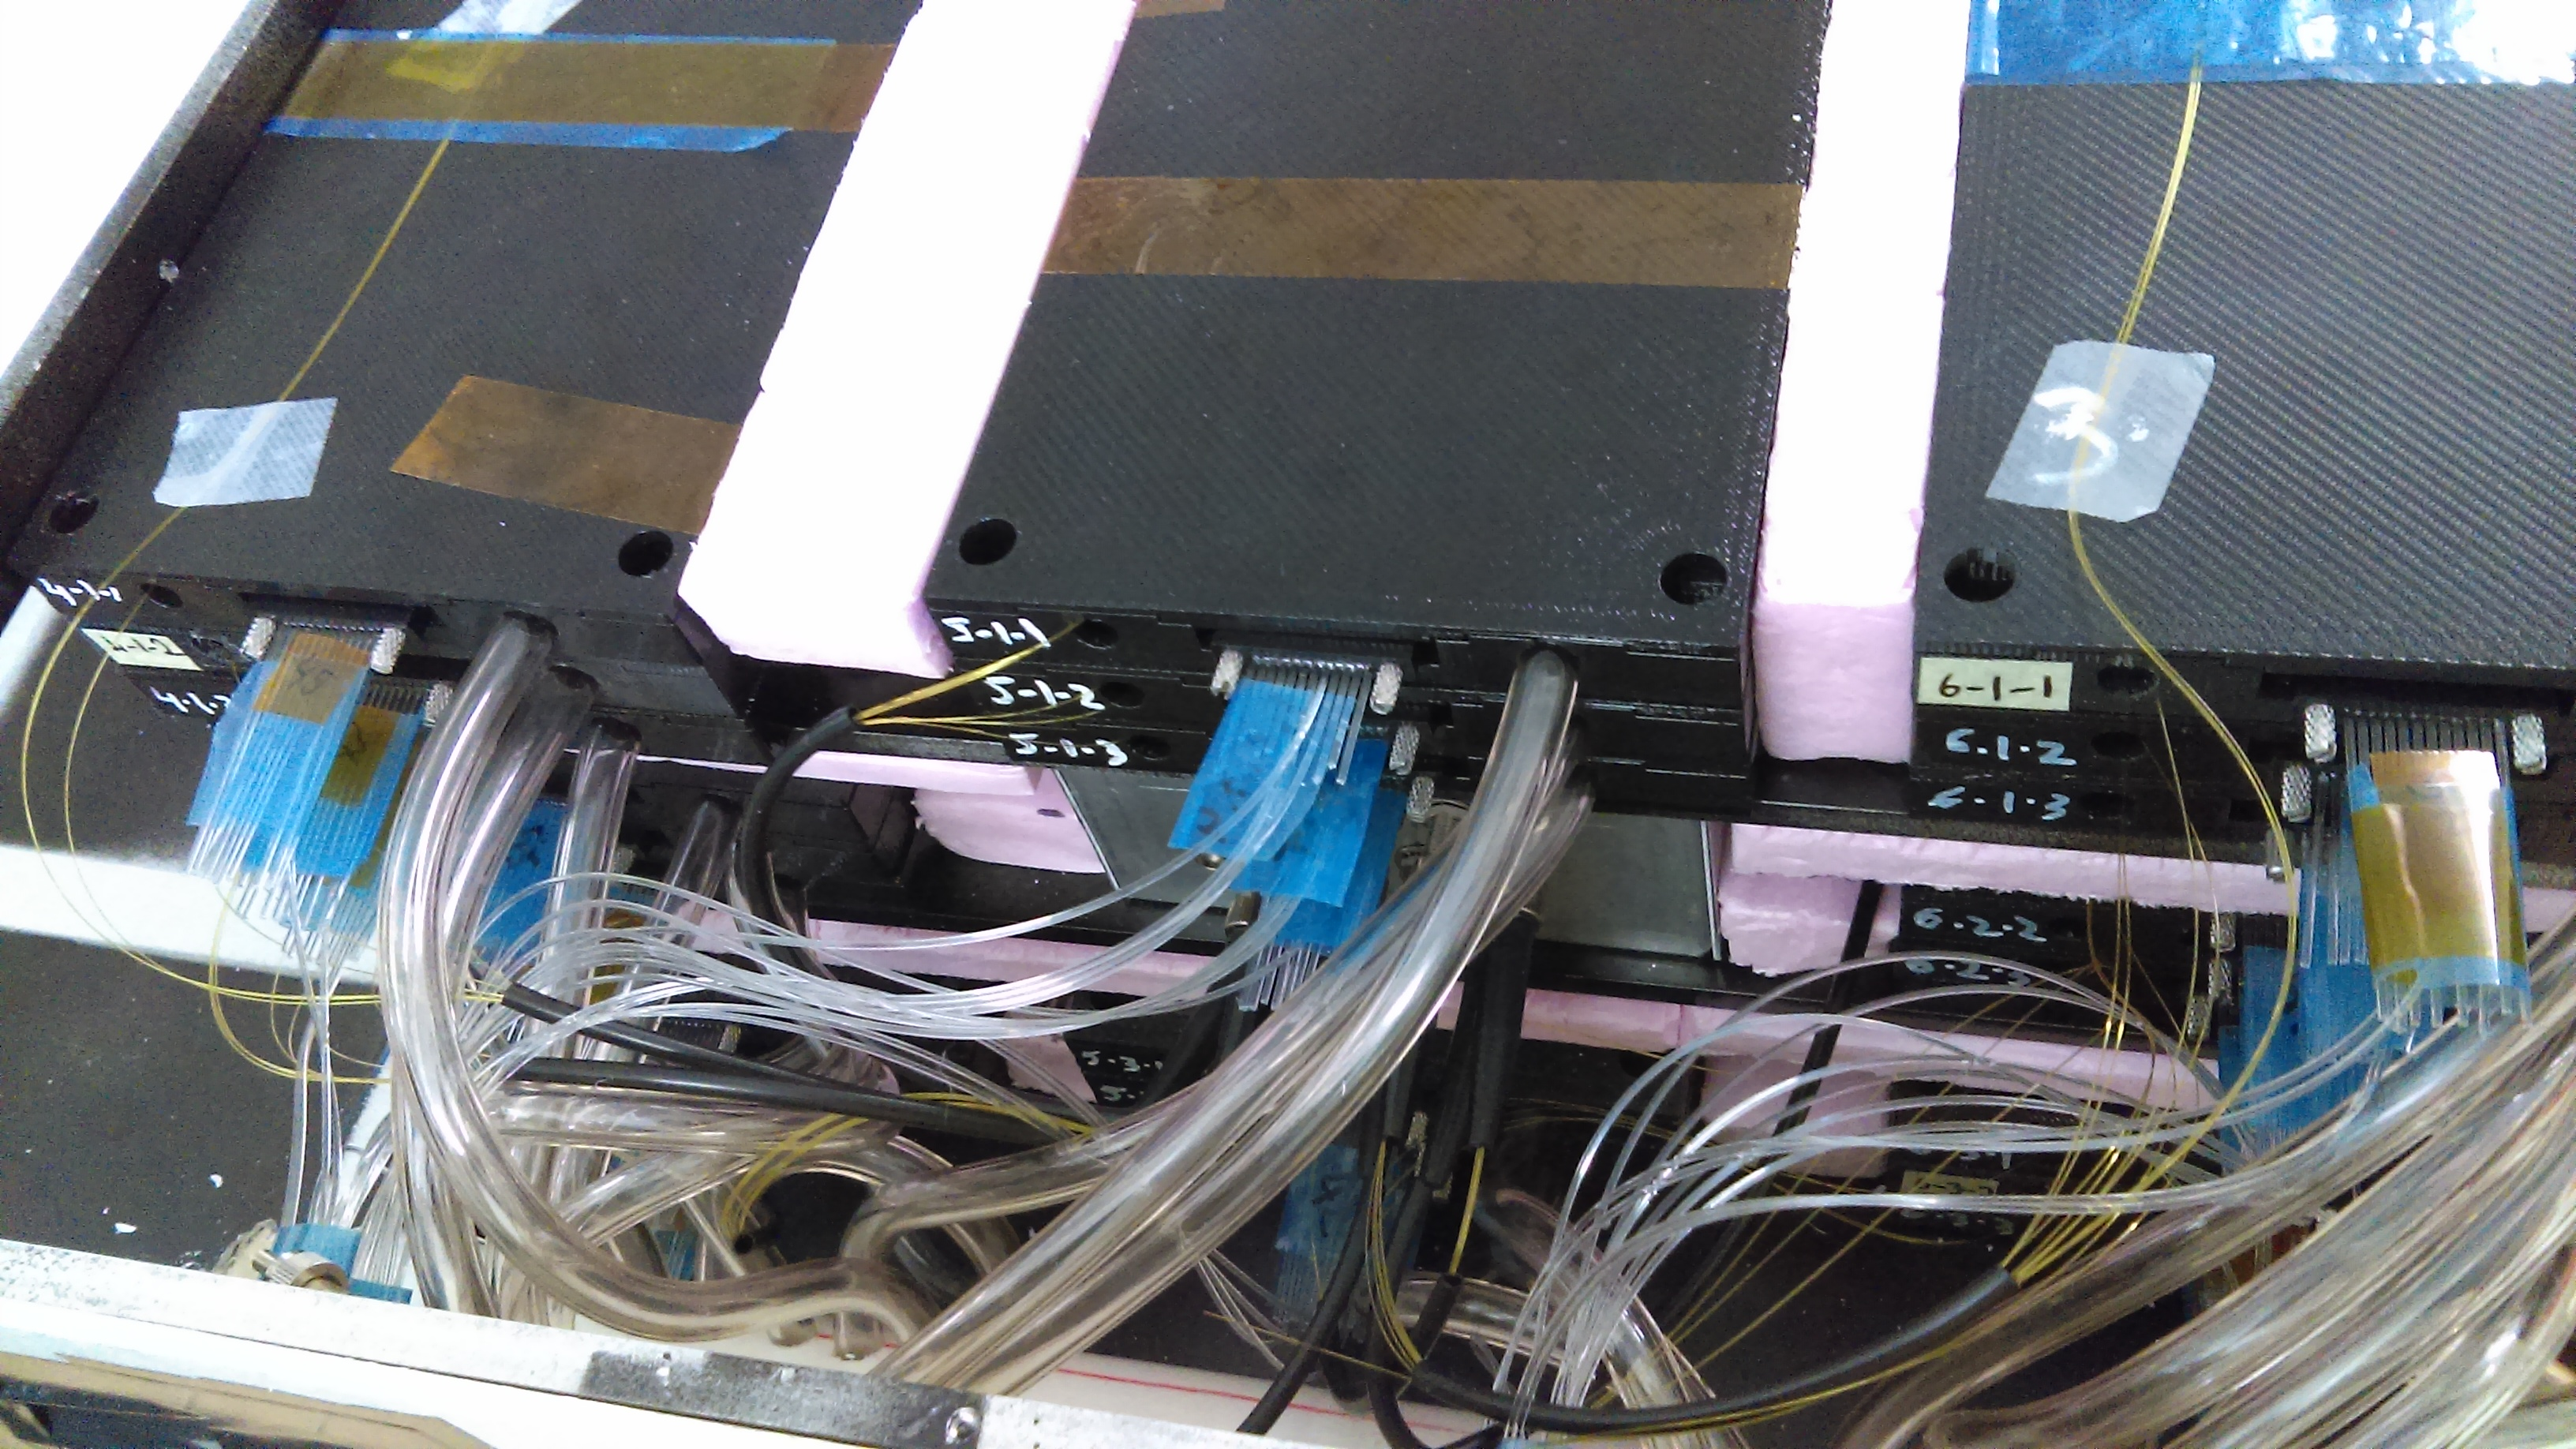
\includegraphics[width=0.8\textwidth]{figures/dark-box-2}
\caption{Zoomed-in view of the interior of a Dark Box. A cluster of clear fibers (reinforced by blue tape) interfaces with the output connector of each cassette. The laser input fibers are thin and yellow in colour; extra, unused laser fibers can be seen taped to the top wall of some cassettes. Thick transparent plastic tubes distribute dry air into the cassettes.}
\label{fig:dark-box-2}
\end{center}
\end{figure}

\subsection{Signal readout\label{sec:setup-readout}}
The clear fibers coming from the Dark Boxes are connected to Phase I HE readout modules (RMs) that receive the scintillation light carried by the clear fibers. The RMs used in this study have a special 1-to-1 optical decoding unit design, meaning that each incoming clear fiber shines onto one unique SiPM inside the RM. Thus, each individual tile (sigma, finger, or other) is read out by a single SiPM channel in an RM. Two RMs are used in the readout, one for each Dark Box; the RM dedicated to Dark Box 1 is referred to as RM1, and RM2 reads out Dark Box 2. Each RM has a total of 48 readout channels. The bias voltages of the SiPMs have been calibrated so that the gain is 47.44 fC with a standard deviation of 2.1\% (see Figure~\ref{fig:gaindist}).

\begin{figure}[hbtp]
\begin{center}
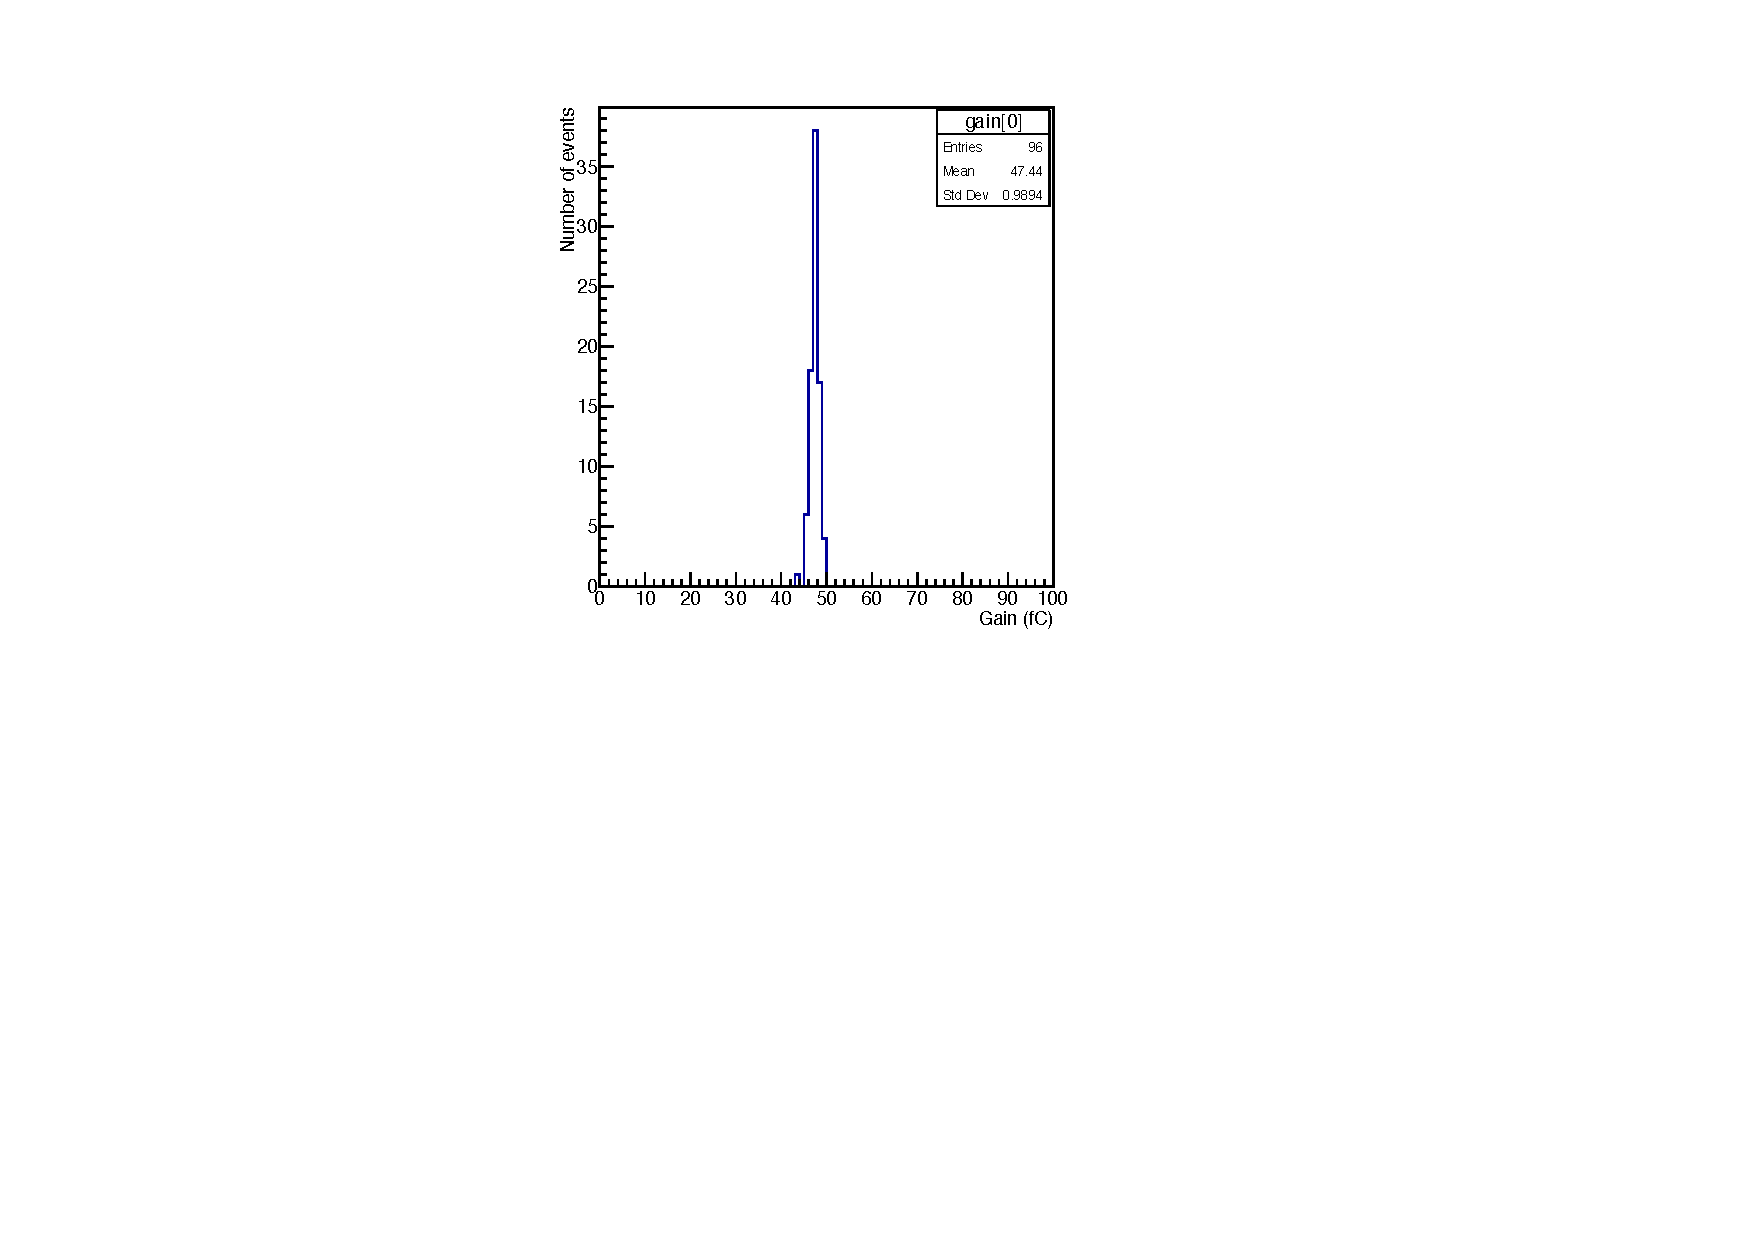
\includegraphics[width=0.8\textwidth]{figures/Run280646_RM1and2_Gains}
\caption{Gain distribution for all channels of RMs 1 and 2 combined (a total of 96 channels) at the start of data-taking with the CRF setup.}
\label{fig:gaindist}
\end{center}
\end{figure}

Charge-integrating QIE11 ADCs digitize the SiPM analog signals, which are then received by a microTCA HCAL Trigger and Readout ($\mu$HTR) card. A new generation Clock and Control Module (ngCCM) controls the CRF front-end. In addition to studying the radiation tolerance properties of upgrade scintillator material candidates, this experiment also serves as a trial run of these Phase I HE front-end and back-end electronics in the experimental cavern.

\subsection{Reference tiles\label{sec:setup-reftiles}}

Throughout the duration of the experiment, the laser amplitude changed dramatically from run to run, due to depletion and refilling of the laser gas. This variation in the measured signal from the tiles from run to run has been taken into account through the use of a reference tile, located outside of CRF and not exposed to a significant dose, but otherwise sharing the same laser and readout pathways as the other channels. In every run, the signal measured in each tile would be normalized to the reference tile signal, thus cancelling out the signal amplitude fluctuation due to the status of the laser gas.

Two reference tiles were used in this experiment. They were located in the TOTEM rack, where the CRF readout box containing the RMs was held. However, the amount of radiation in tis zone was not correctly estimated before the start of the experiment and was actually an order of magnitude higher than expected, reaching a fluence of roughly 1-2$\cdot10^{10}$ neutrons/cm$^{2}$. This caused two important complications. The first was that the SiPMs were damaged by the radiation, and their single photoelectron spectra were progressively drowned by increasing dark current. The second was one of the reference tiles received a significant amount of damage, as evidenced by an exponential decay in its light yield in comparison with the other tile during the irradiation period.

Due to the lack of distinguishable photoelectron peaks after the first 2.3 fb$^{-1}$ of integrated luminosity, the SiPM gain for each subsequent run could not be calculated from the position of the pedestal and first photoelectron peak. However, an alternate method of measuring the gain was developed, and the gain was shown to be reasonably stable during the irradiation period. The damage to one of the reference tiles meant that it could not be relied upon to normalize the light yield of the CRF tiles. Thus, all the tiles were normalized to the signal from the other, less-damaged reference tile.

\section{Analysis\label{sec:analysis}}

To study the effect of radiation damage on scintillation yield, the laser response in each tile was measured periodically as the total integrated dose accumulated. Thus it is necessary to relate the relative light yield of each tile in a given run to its absorbed dose, rather than the delivered luminosity. The integrated luminosities at the time of each measurement were converted to integrated doses based on film dosimetry measurements in the CRF performed in 2015~\cite{CMS-DN-2018-008}. After a total integrated luminosity of 10.03 \fbinv, the closest tiles to the beam received a dose of approximately 6.04 Mrad, while the farthest tiles received a dose of approximately 1.53 Mrad.
%N.B. The max and min total doses quoted here are for SCSN81 tiles only.
%The remaining relative light yield as a function of dose for a selection of channels is shown in Figure~\ref{remaining_relative_dose}.

\subsection{Analysis procedure\label{sec:ana-proc}} 

In each event, the laser response in each channel is characterized by summing the charge collected in a window of 4 time slices around the pulse peak, beginning with the time slice immediately before the peak time slice and continuing through the two time slices after the peak. The first two time slices in the readout window are always avoided since they sometimes contained huge spikes due to a firmware bug present during data-taking. Since the SiPM+QIE11 pedestal currents are non-neglible and also grow with total received dose, average pedestals for each channel and capacitor were measured at the time of each laser run and subtracted from the charge observed during the laser pulses. Example average pulse shapes and pedestals can be seen in Figures~\ref{pulse0ifb},~\ref{pulse2p7ifb} and~\ref{pulse9p5ifb} for a selection of channels at various doses. This pedestal-subtracted pulse size integrated over four time slices is a measure of the tile's light yield.

During each dedicated laser run, the laser is fired into the CRF tiles 10000 times. Thus, for a given run, the light yield of a tile is taken as the mean of the distribution of 10000 pedestal-subtracted pulse size measurements. This figure is then divided by the mean light yield of the reference tile in that same run to factor out run-to-run variation due to the laser amplitude; this will be referred to as the normalized light yield L.% The charge progressions before and after normalization to the reference tile are shown in Figures~\ref{energy_raw} and Figures~\ref{energy_norm}.
%%The resulting relative charge progressions over X \fbinv are shown in Fig...

To assess the drop in light yield L(\textit{d}) of a tile relative after dose \textit{d} to its pre-irradiation light yield taken on day 0 (defined as the day when the tiles were installed on the CASTOR table), the normalized light yield of the tile is divided by the normalized light yield L(0) from day 0, to yield the relative light yield L(\textit{d})/L(0) as expressed in Equation~\ref{eq:lightloss}. L(\textit{d})/L(0) is plotted as a function of dose in order to calculate the dose constant for a tile.
%These ratios are shown in Figure~\ref{remaining_relative}.

\begin{figure}[tbp!]
\centering
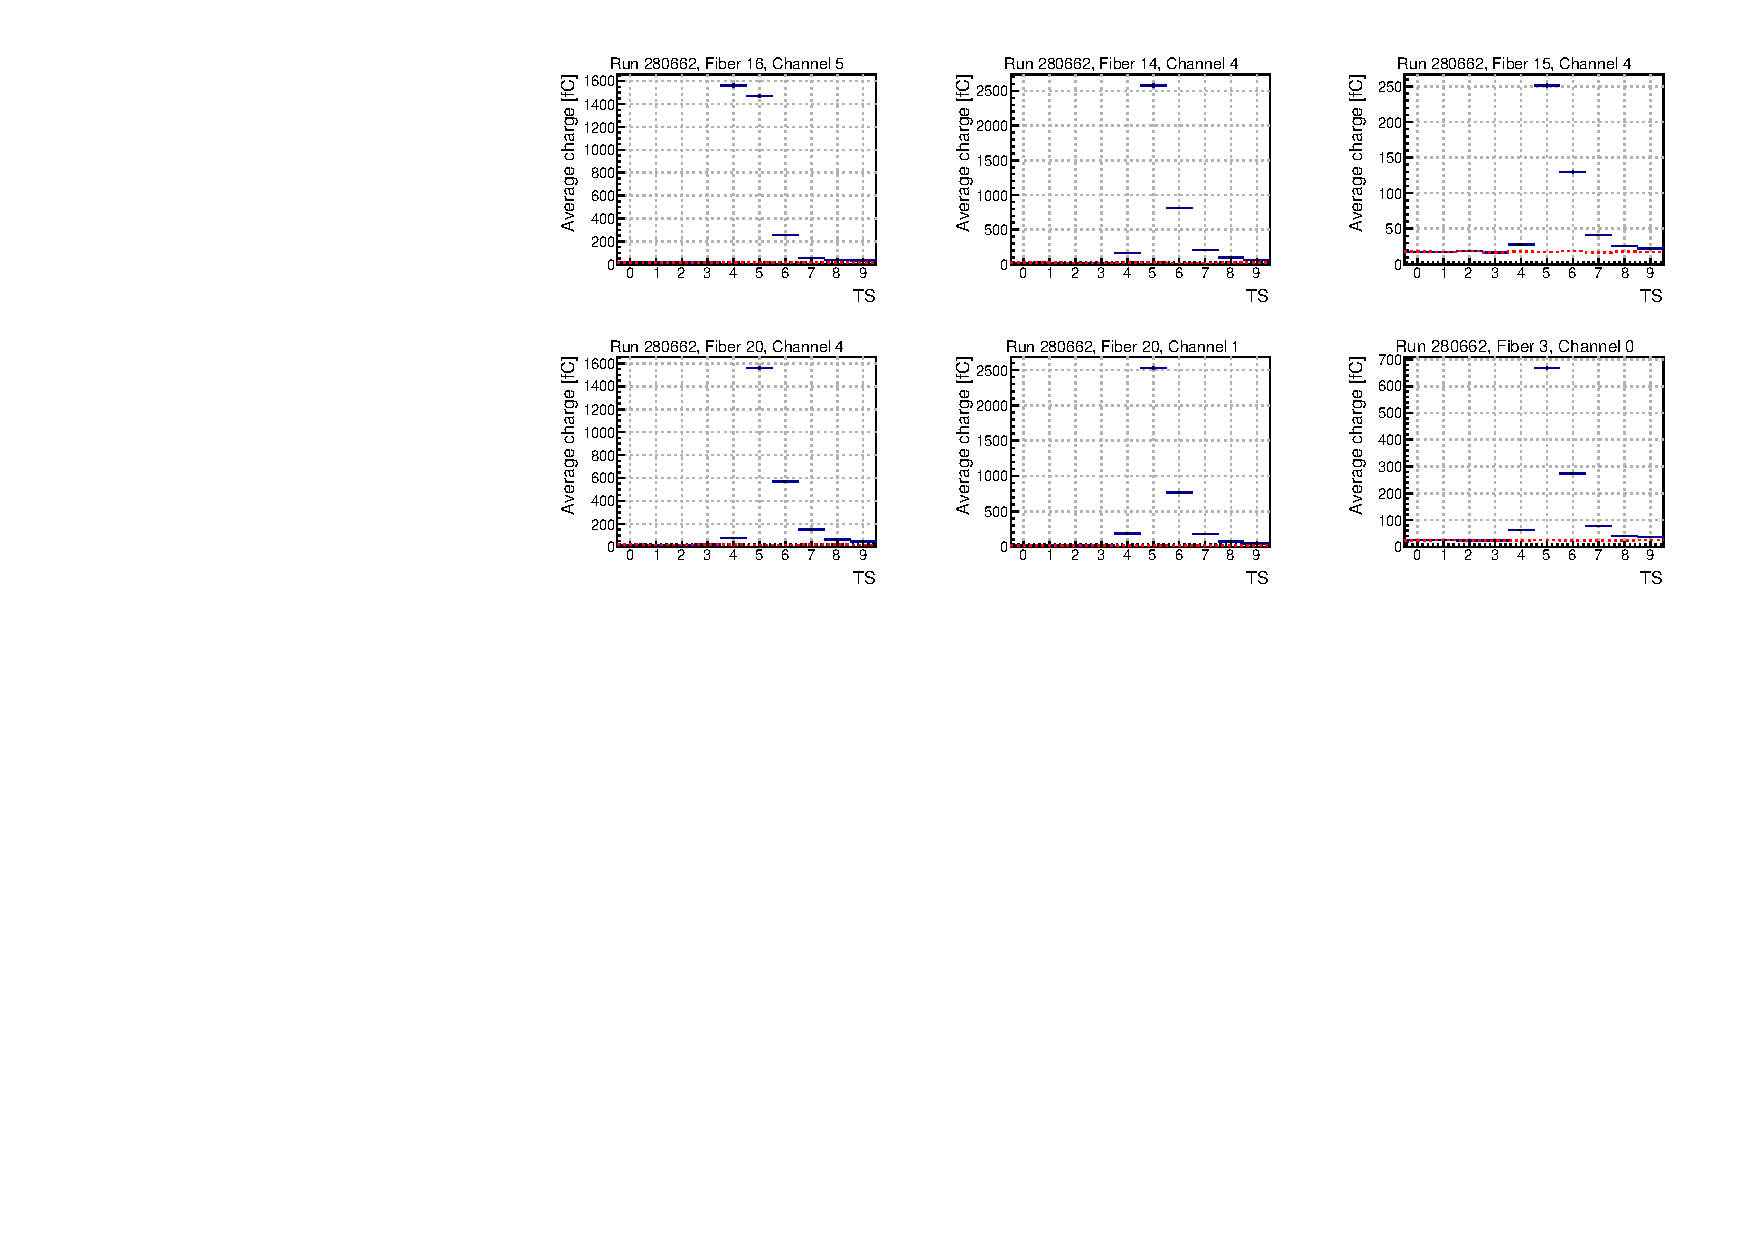
\includegraphics[width=0.97\textwidth]{figures/analysis/Pulse_shape_run280662_bright_SCSN81S.pdf}
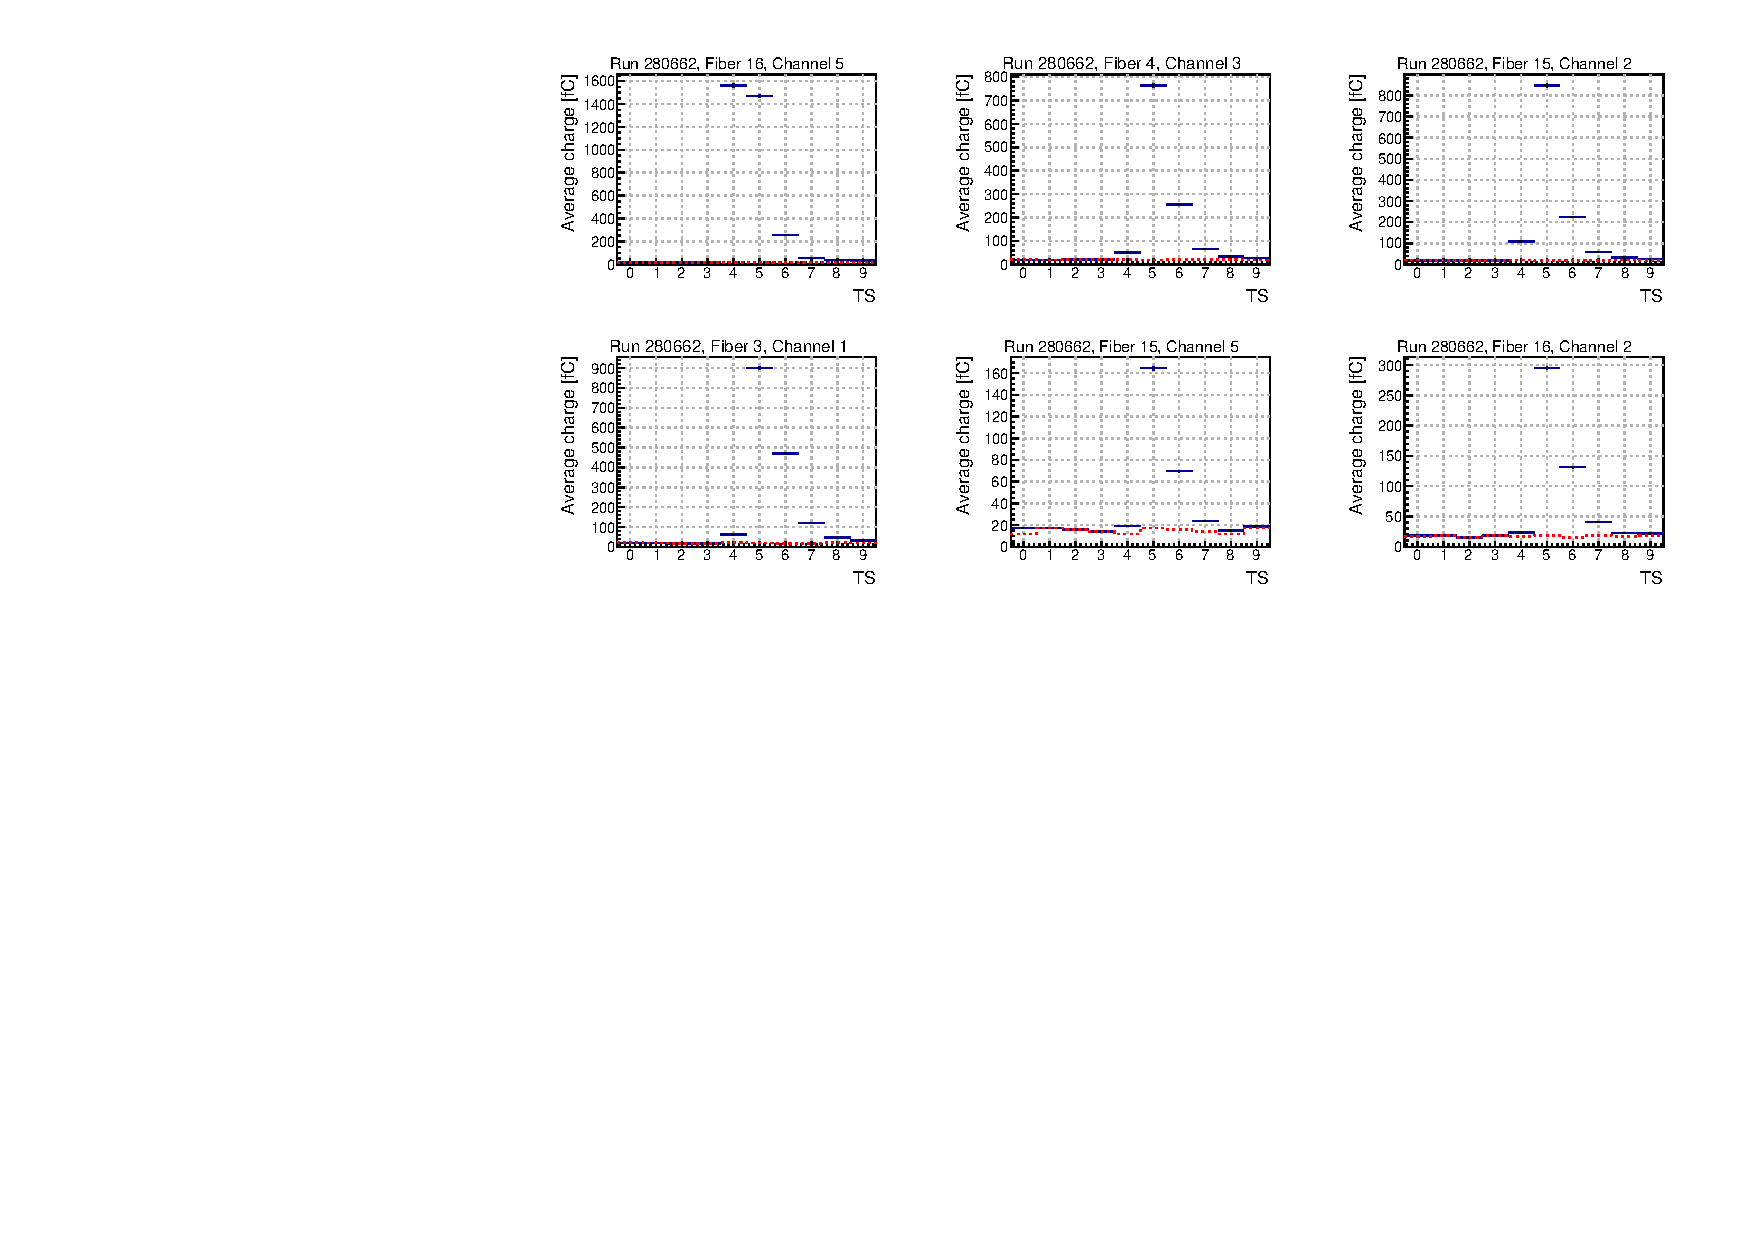
\includegraphics[width=0.97\textwidth]{figures/analysis/Pulse_shape_run280662_bright_others.pdf}
\caption{Average pulse shapes in response to laser (blue) and corresponding pedestals (red) at the time of installation for a selection of SCSN81-S channels (top half) and other materials (bottom half).}
\label{pulse0ifb}
\end{figure} 

\begin{figure}[tbp!]
\centering
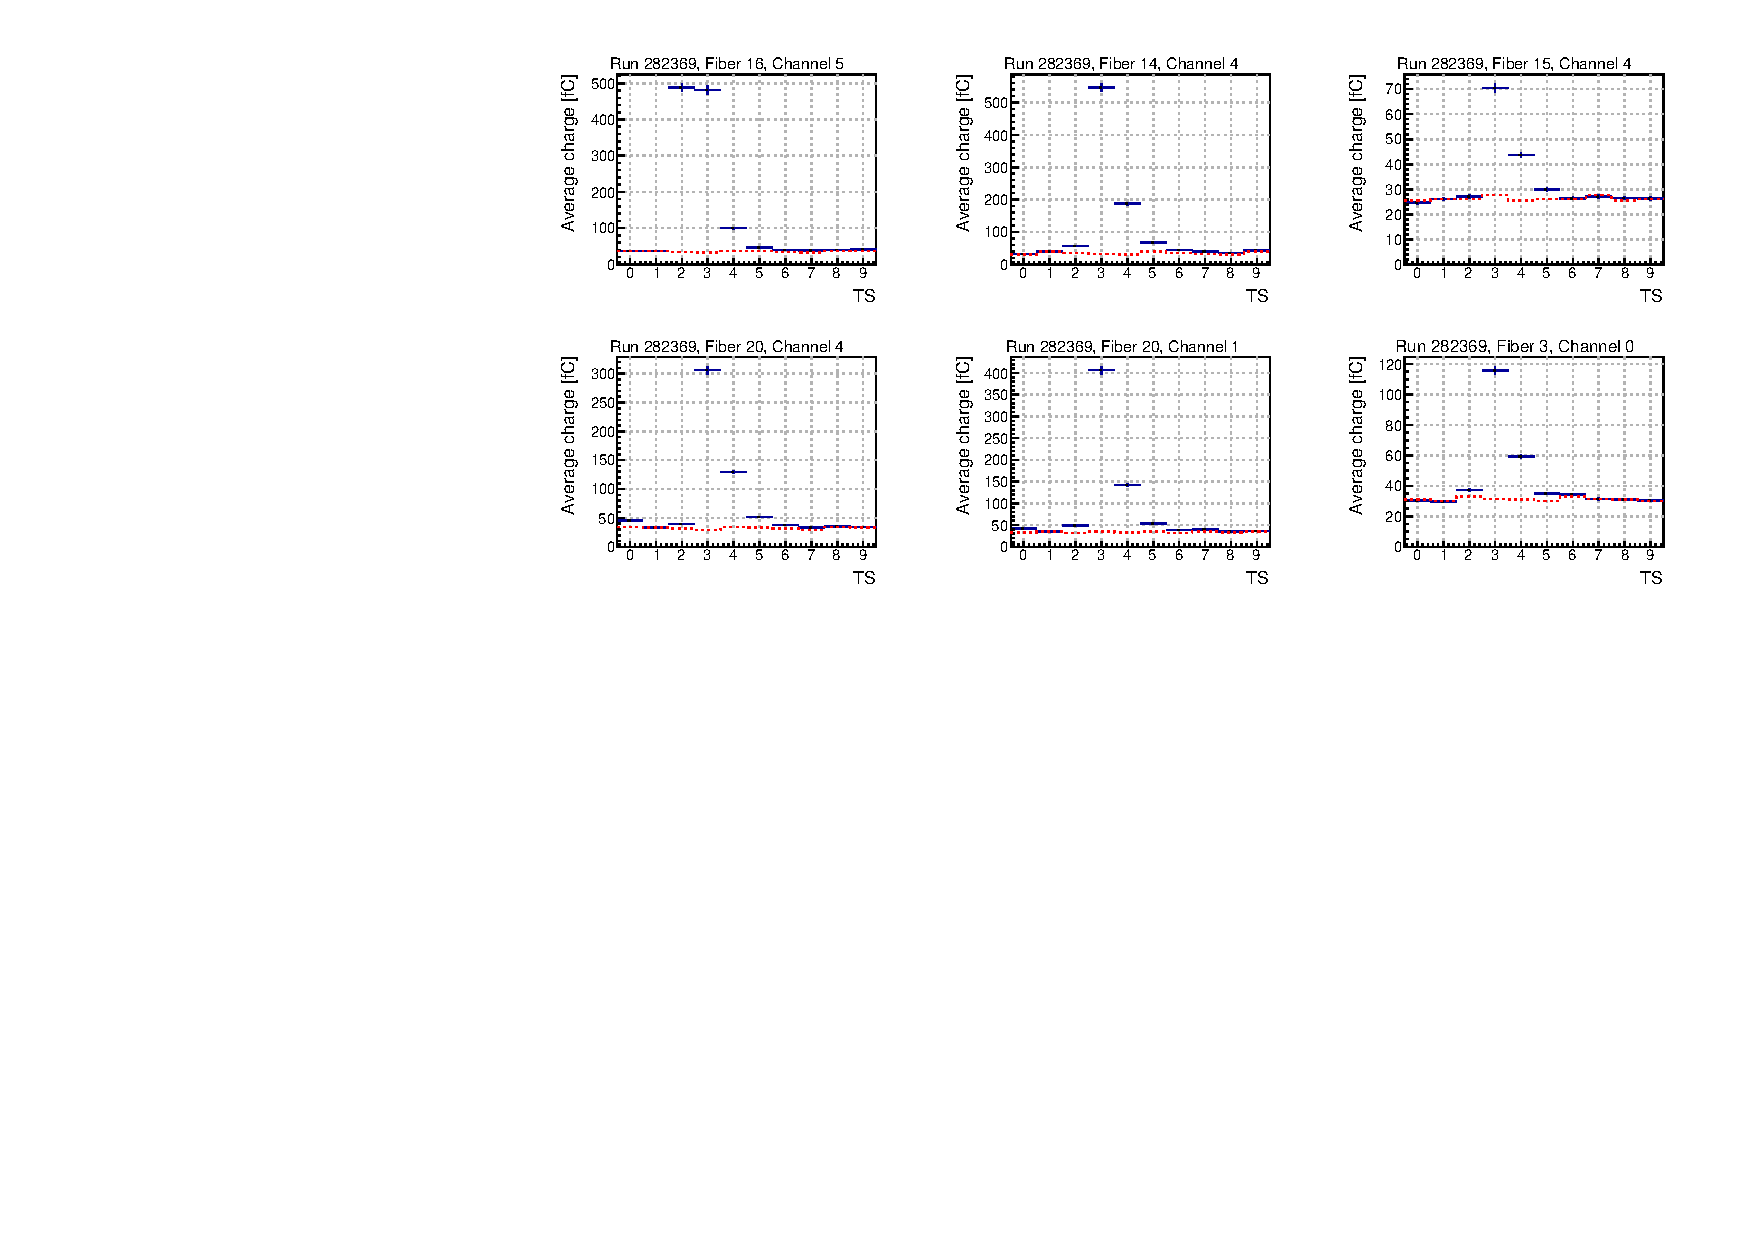
\includegraphics[width=0.97\textwidth]{figures/analysis/Pulse_shape_run282369_bright_SCSN81S.pdf}
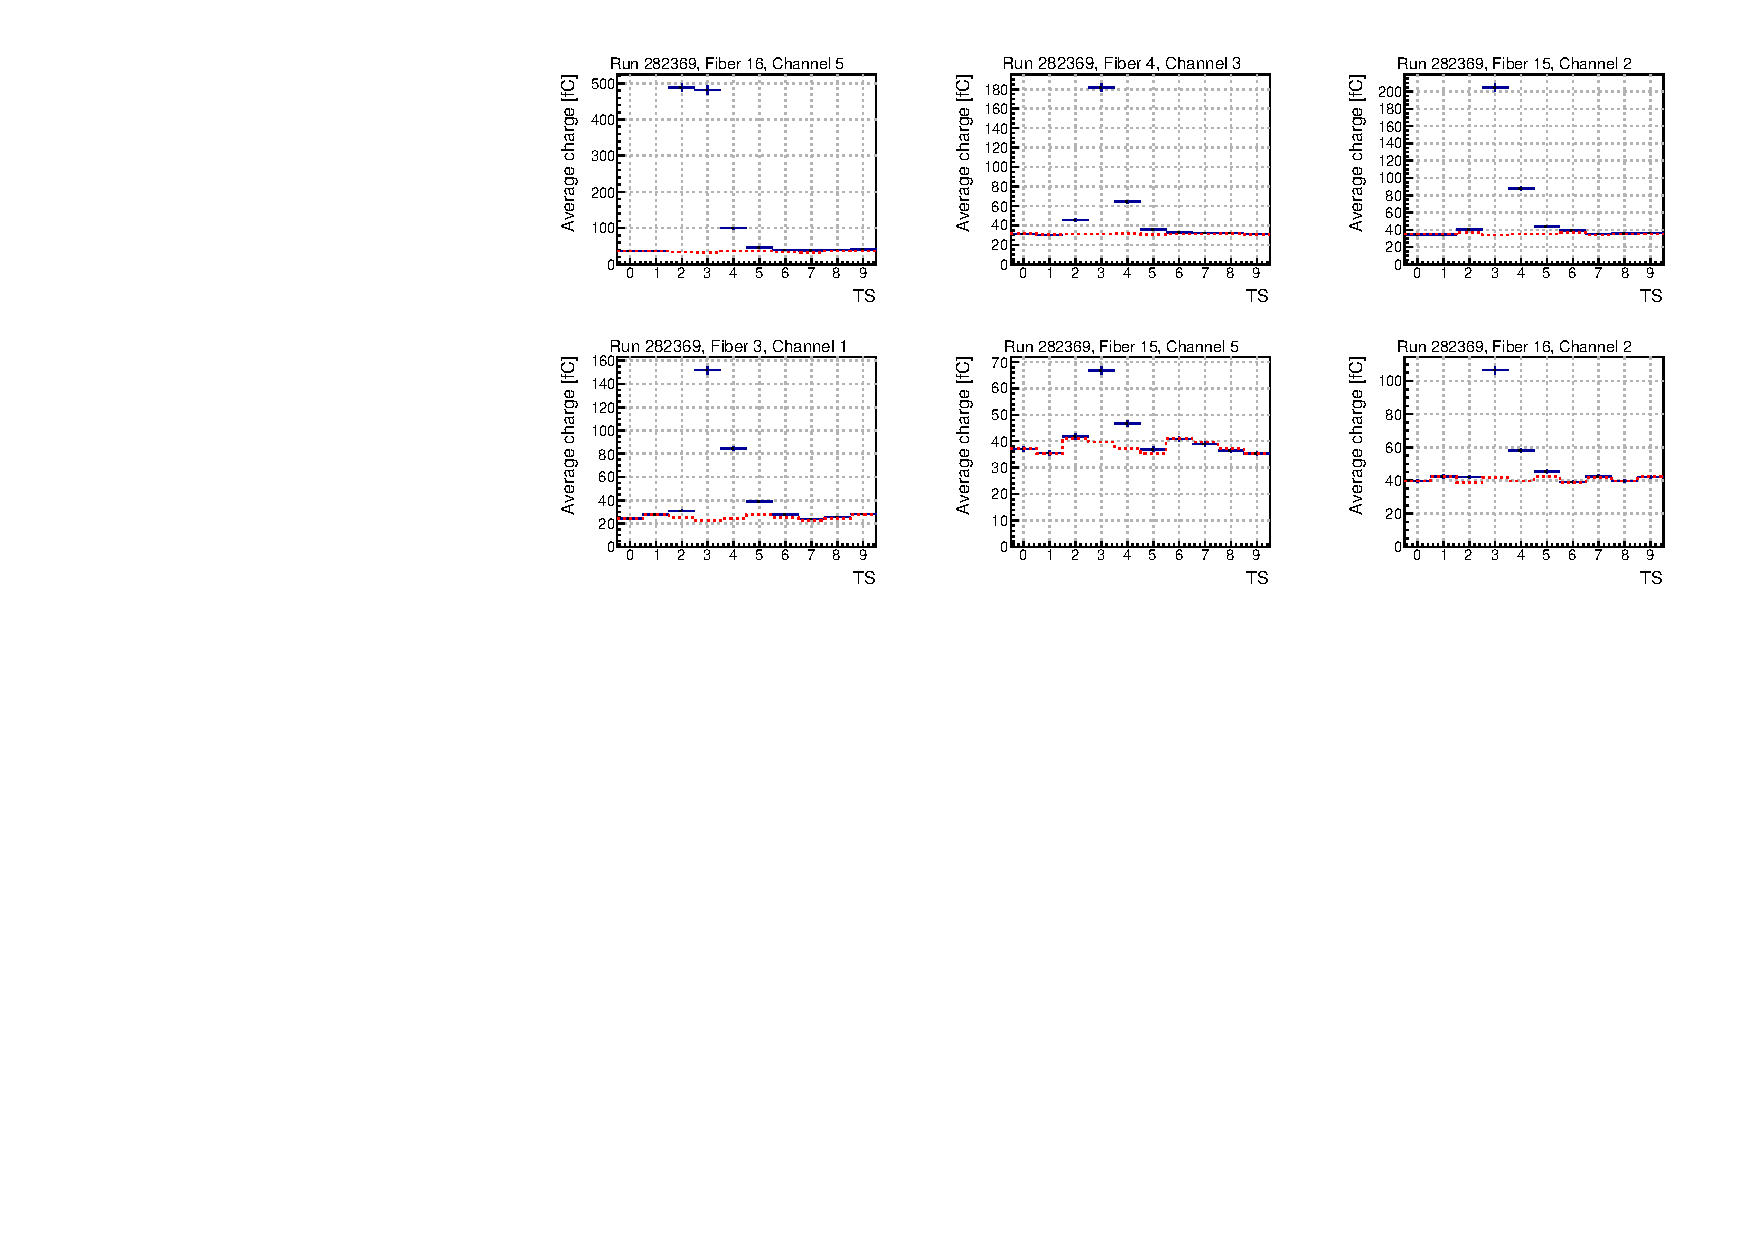
\includegraphics[width=0.97\textwidth]{figures/analysis/Pulse_shape_run282369_bright_others.pdf}
\caption{Average pulse shapes in response to laser (blue) and corresponding pedestals (red) after a delivered luminosity of 2.7 $\fbinv$ for a selection of SCSN81-S channels (top half) and other materials (bottom half).}
\label{pulse2p7ifb}
\end{figure} 

\begin{figure}[tbp!]
\centering
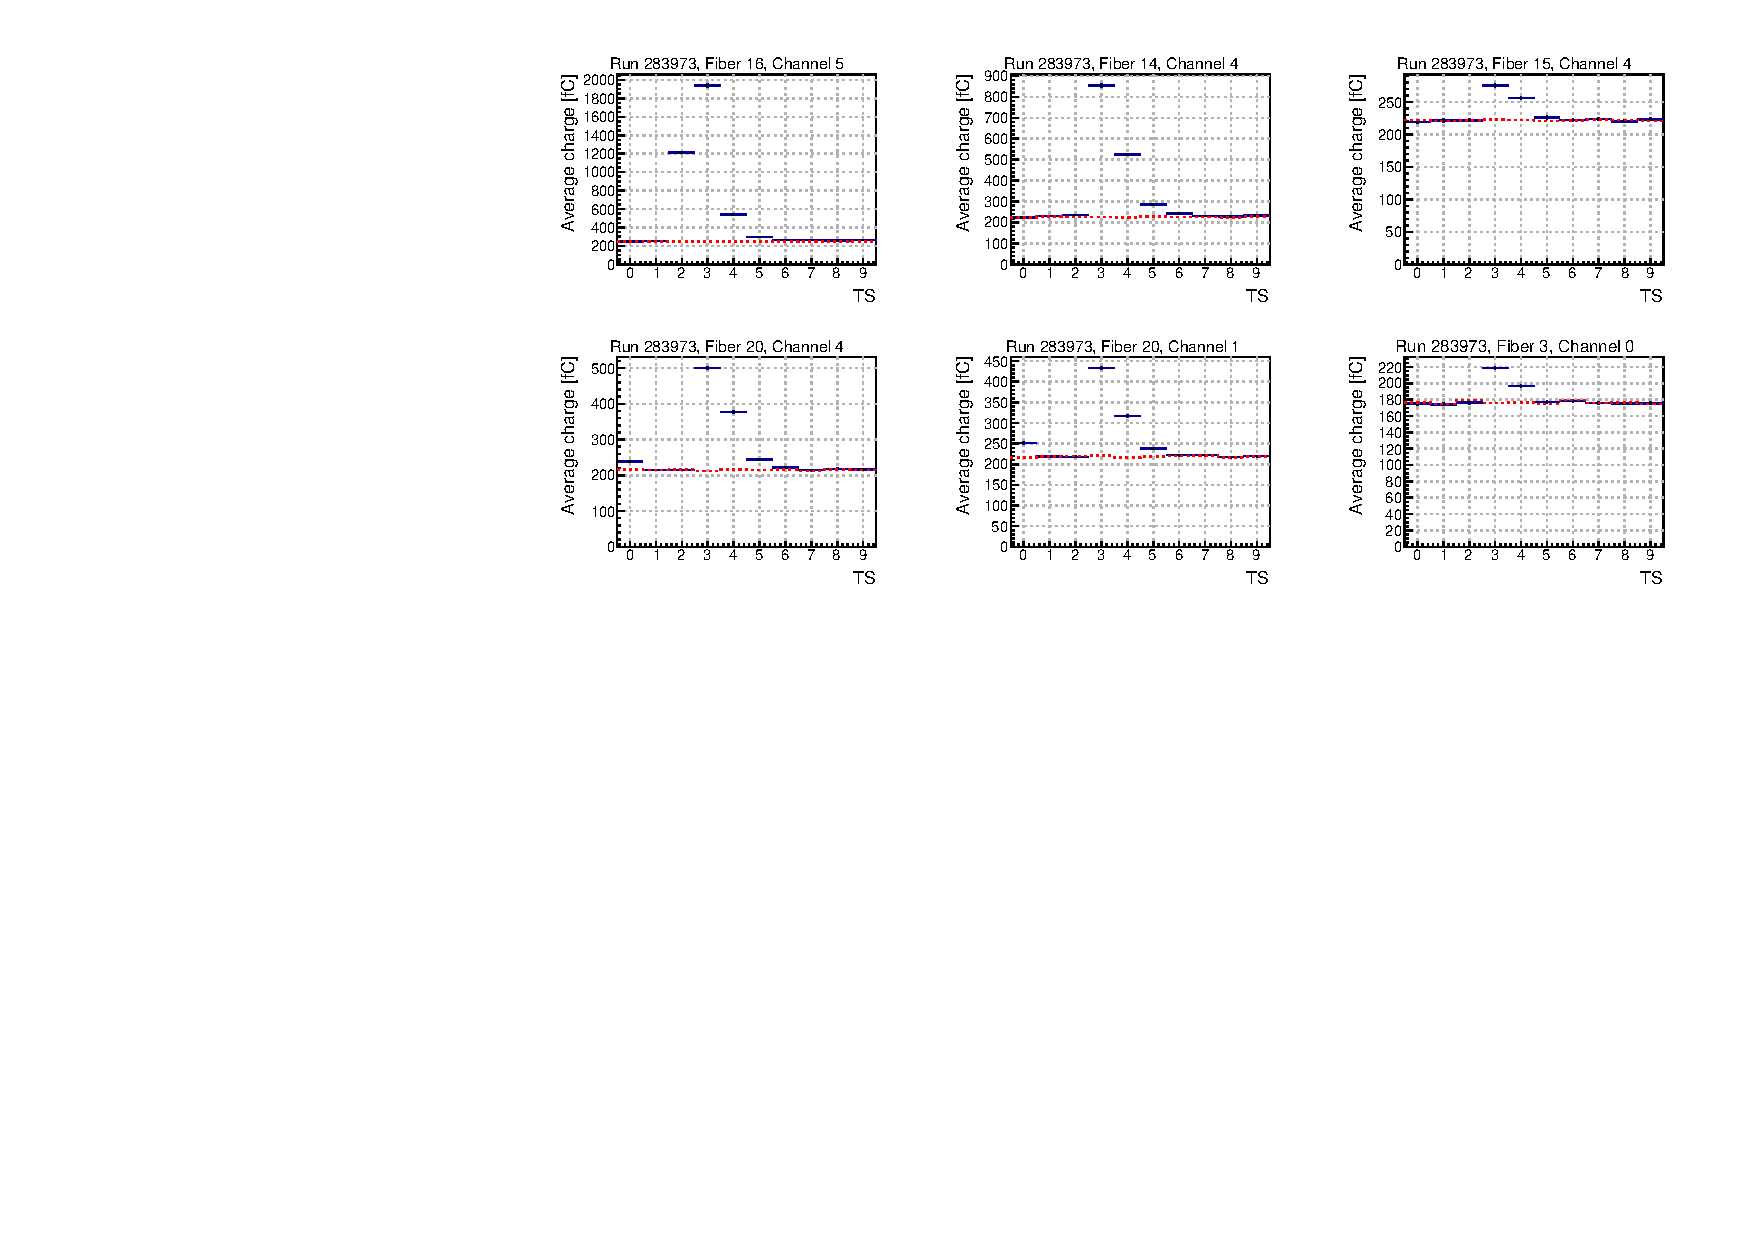
\includegraphics[width=0.97\textwidth]{figures/analysis/Pulse_shape_run283973_bright_SCSN81S.pdf}
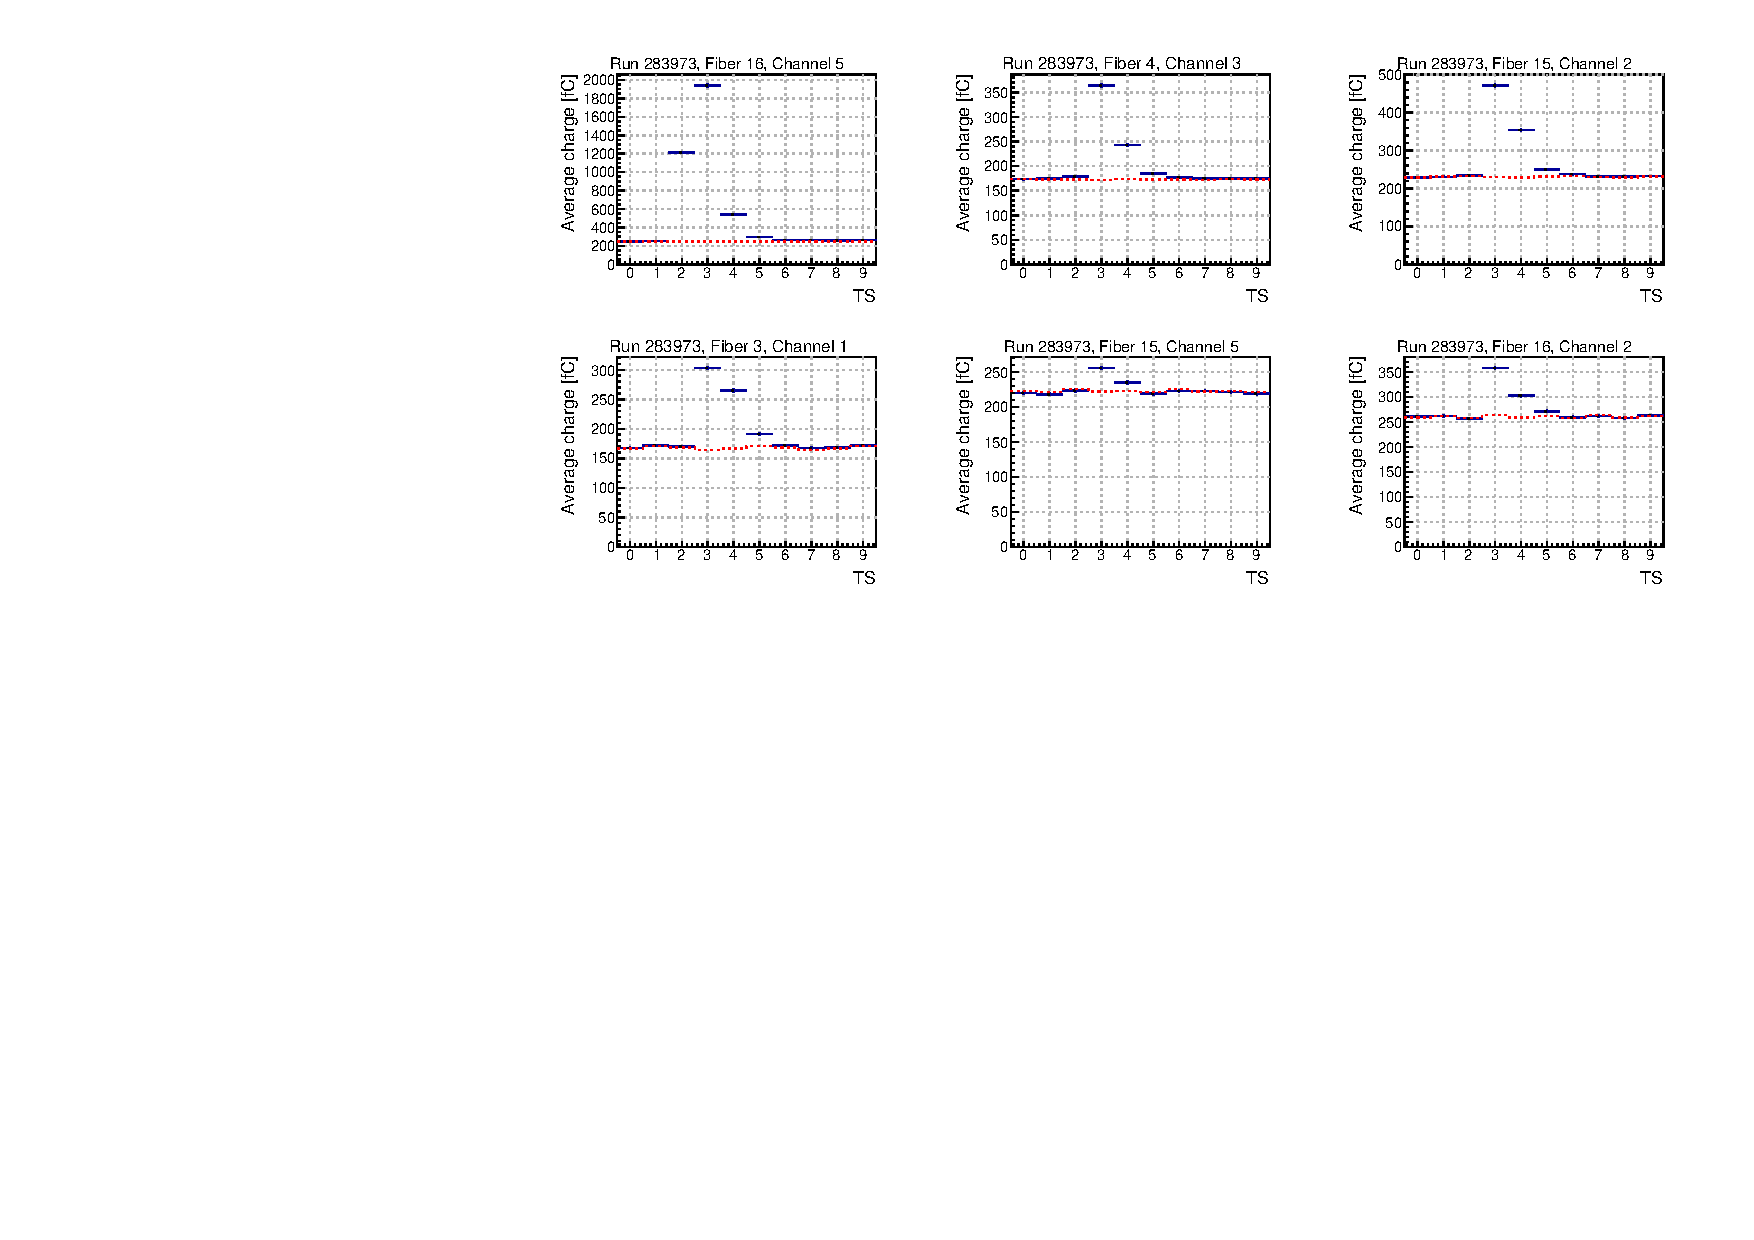
\includegraphics[width=0.97\textwidth]{figures/analysis/Pulse_shape_run283973_bright_others.pdf}
\caption{Average pulse shapes in response to laser (blue) and corresponding pedestals (red) after a delivered luminosity of 9.5 $\fbinv$ for a selection of SCSN81-S channels (top half) and other materials (bottom half).}
\label{pulse9p5ifb}
\end{figure} 

%\begin{figure}[tbp!]
%\centering
%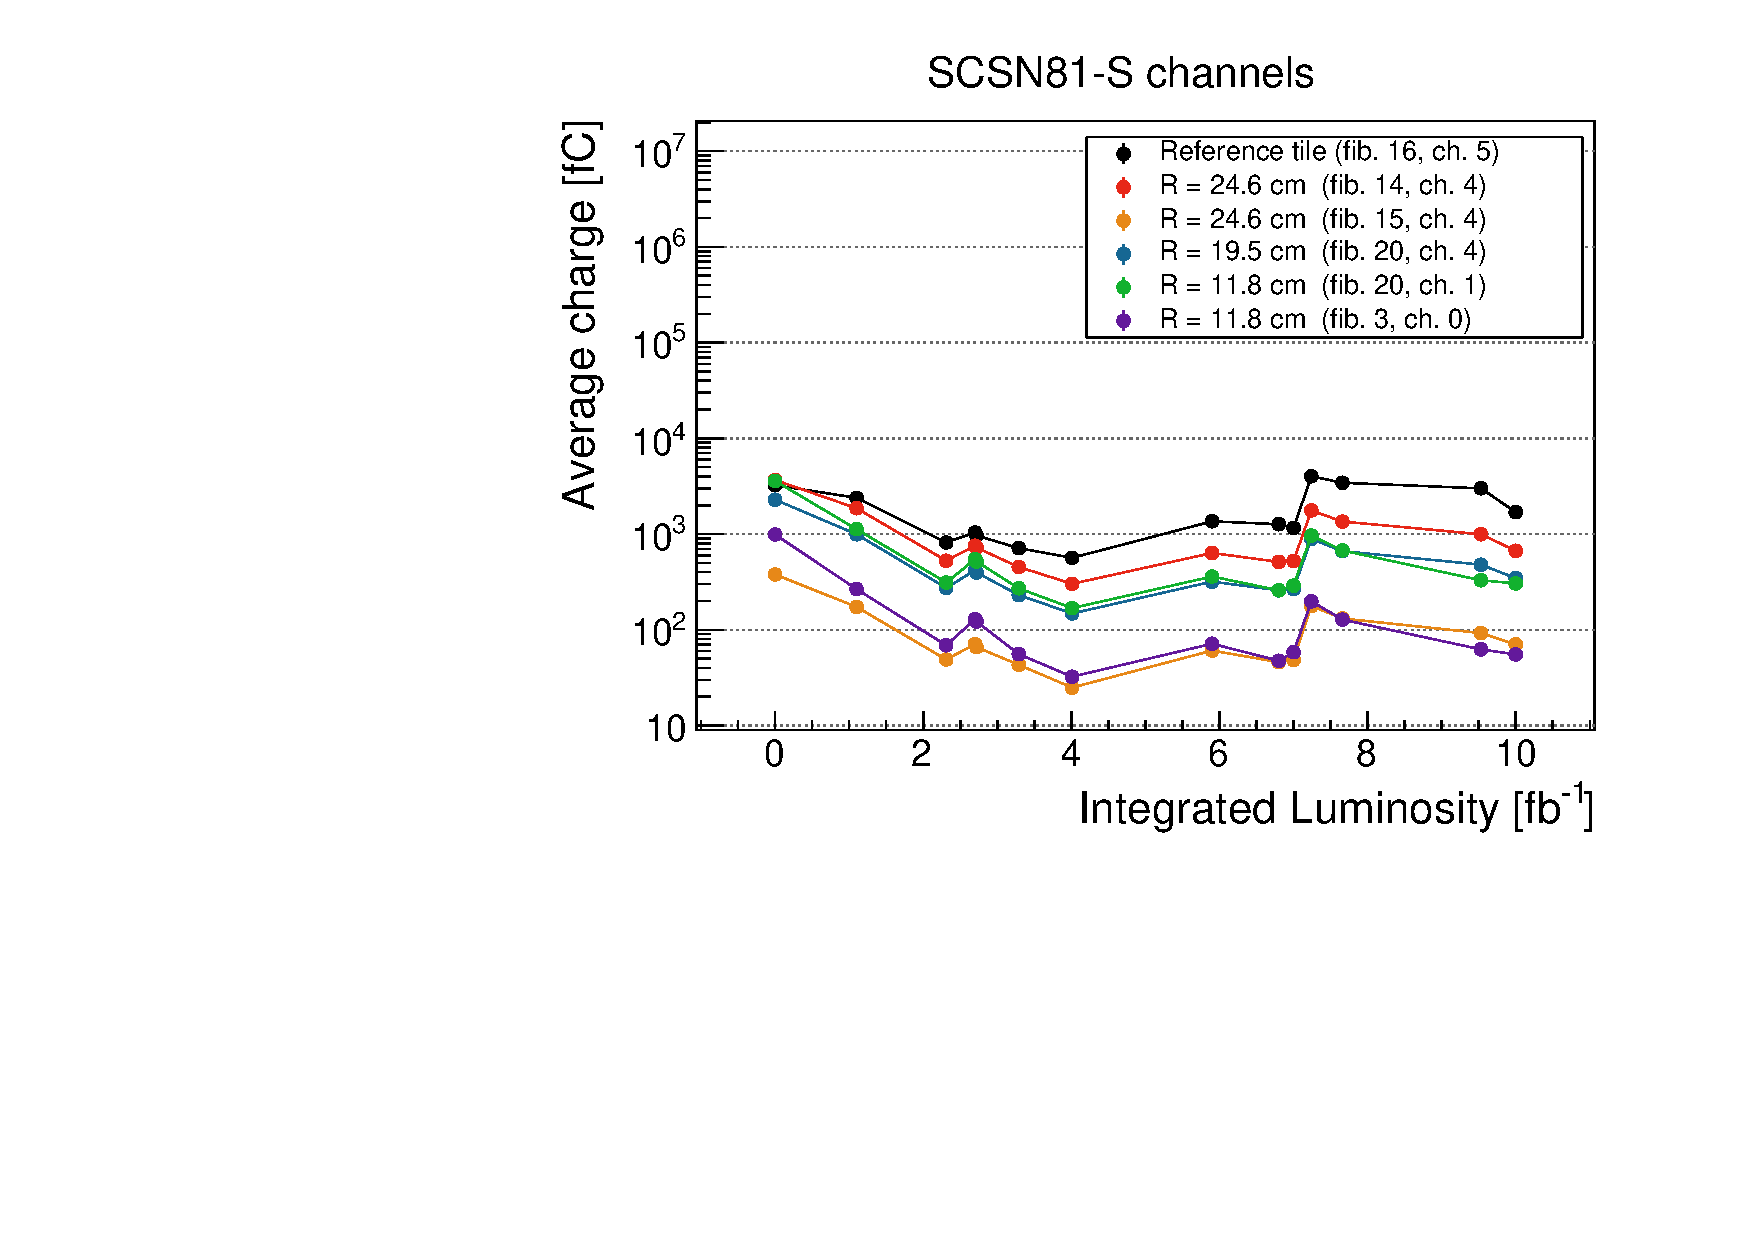
\includegraphics[width=0.46\textwidth]{figures/analysis/log_energy_lasercons_v14__scsnvar_vs_lumi.pdf}
%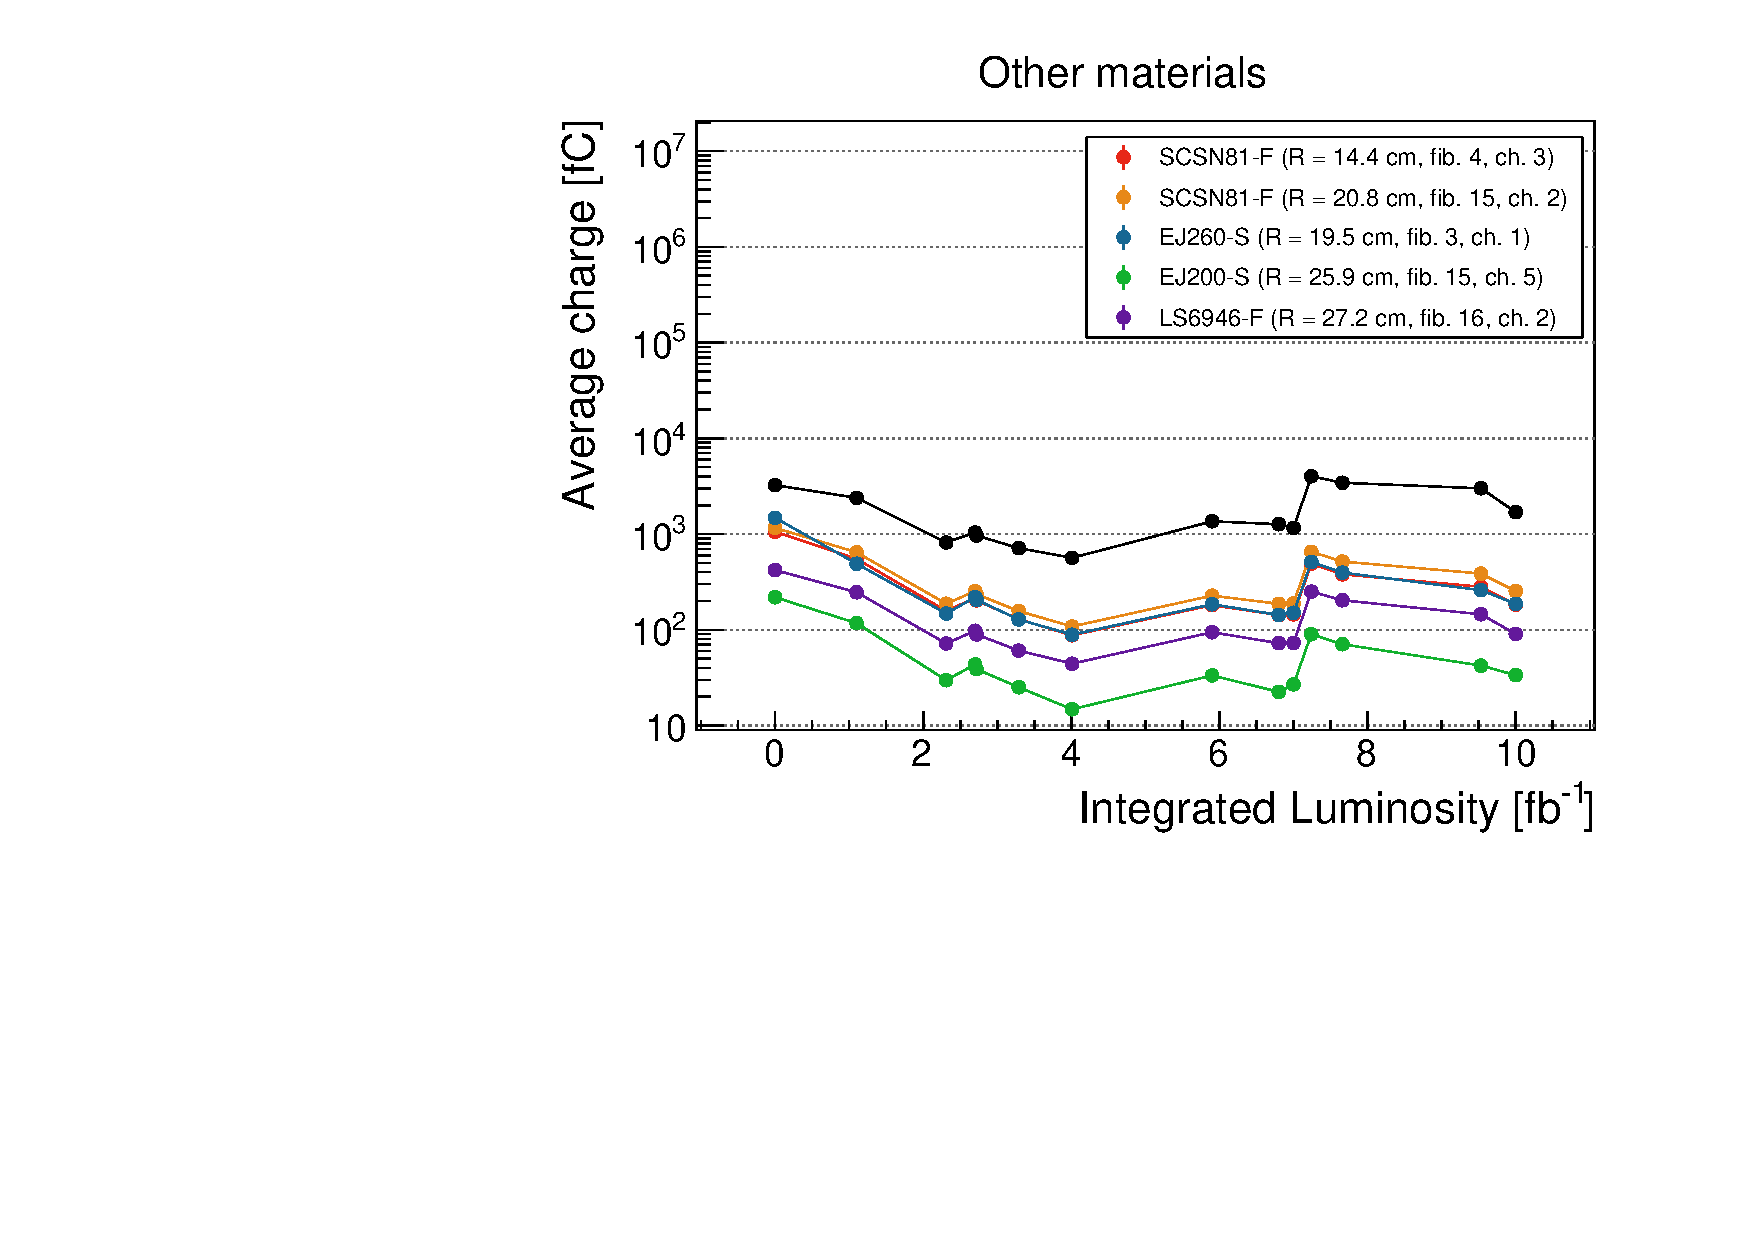
\includegraphics[width=0.46\textwidth]{figures/analysis/log_energy_lasercons_v14__bright_variety_vs_lumi.pdf}
%\caption{Progression of average laser response as a function of delivered luminosity, for a selection of channels. Left: SCSN81-S tiles. Right: variety of alternative tiles. Most variation in time is due to variation in laser amplitude.}
%\label{energy_raw}
%\end{figure}

%\begin{figure}[tbp!]
%\centering
%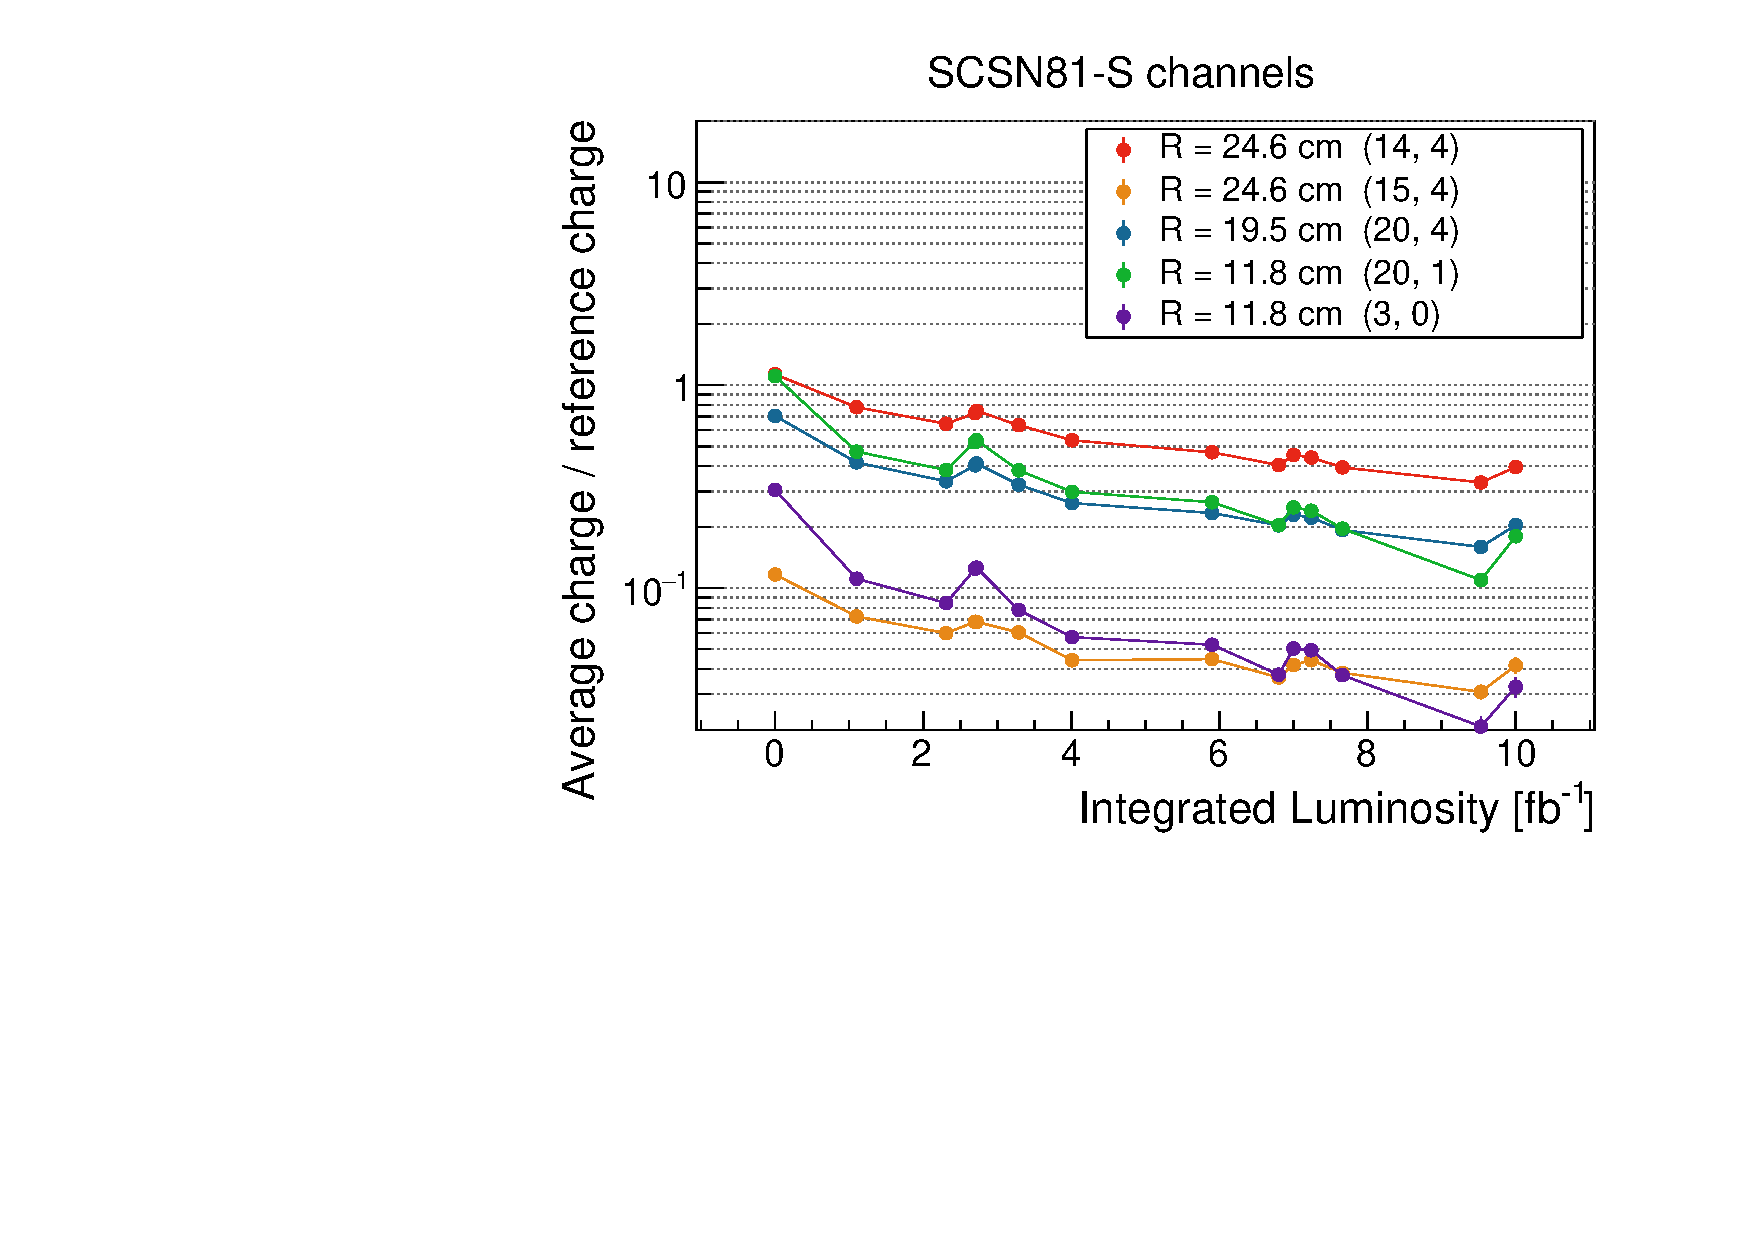
\includegraphics[width=0.46\textwidth]{figures/analysis/log_energy_lasercons_v14__scsnvar_vs_lumi_norm.pdf}
%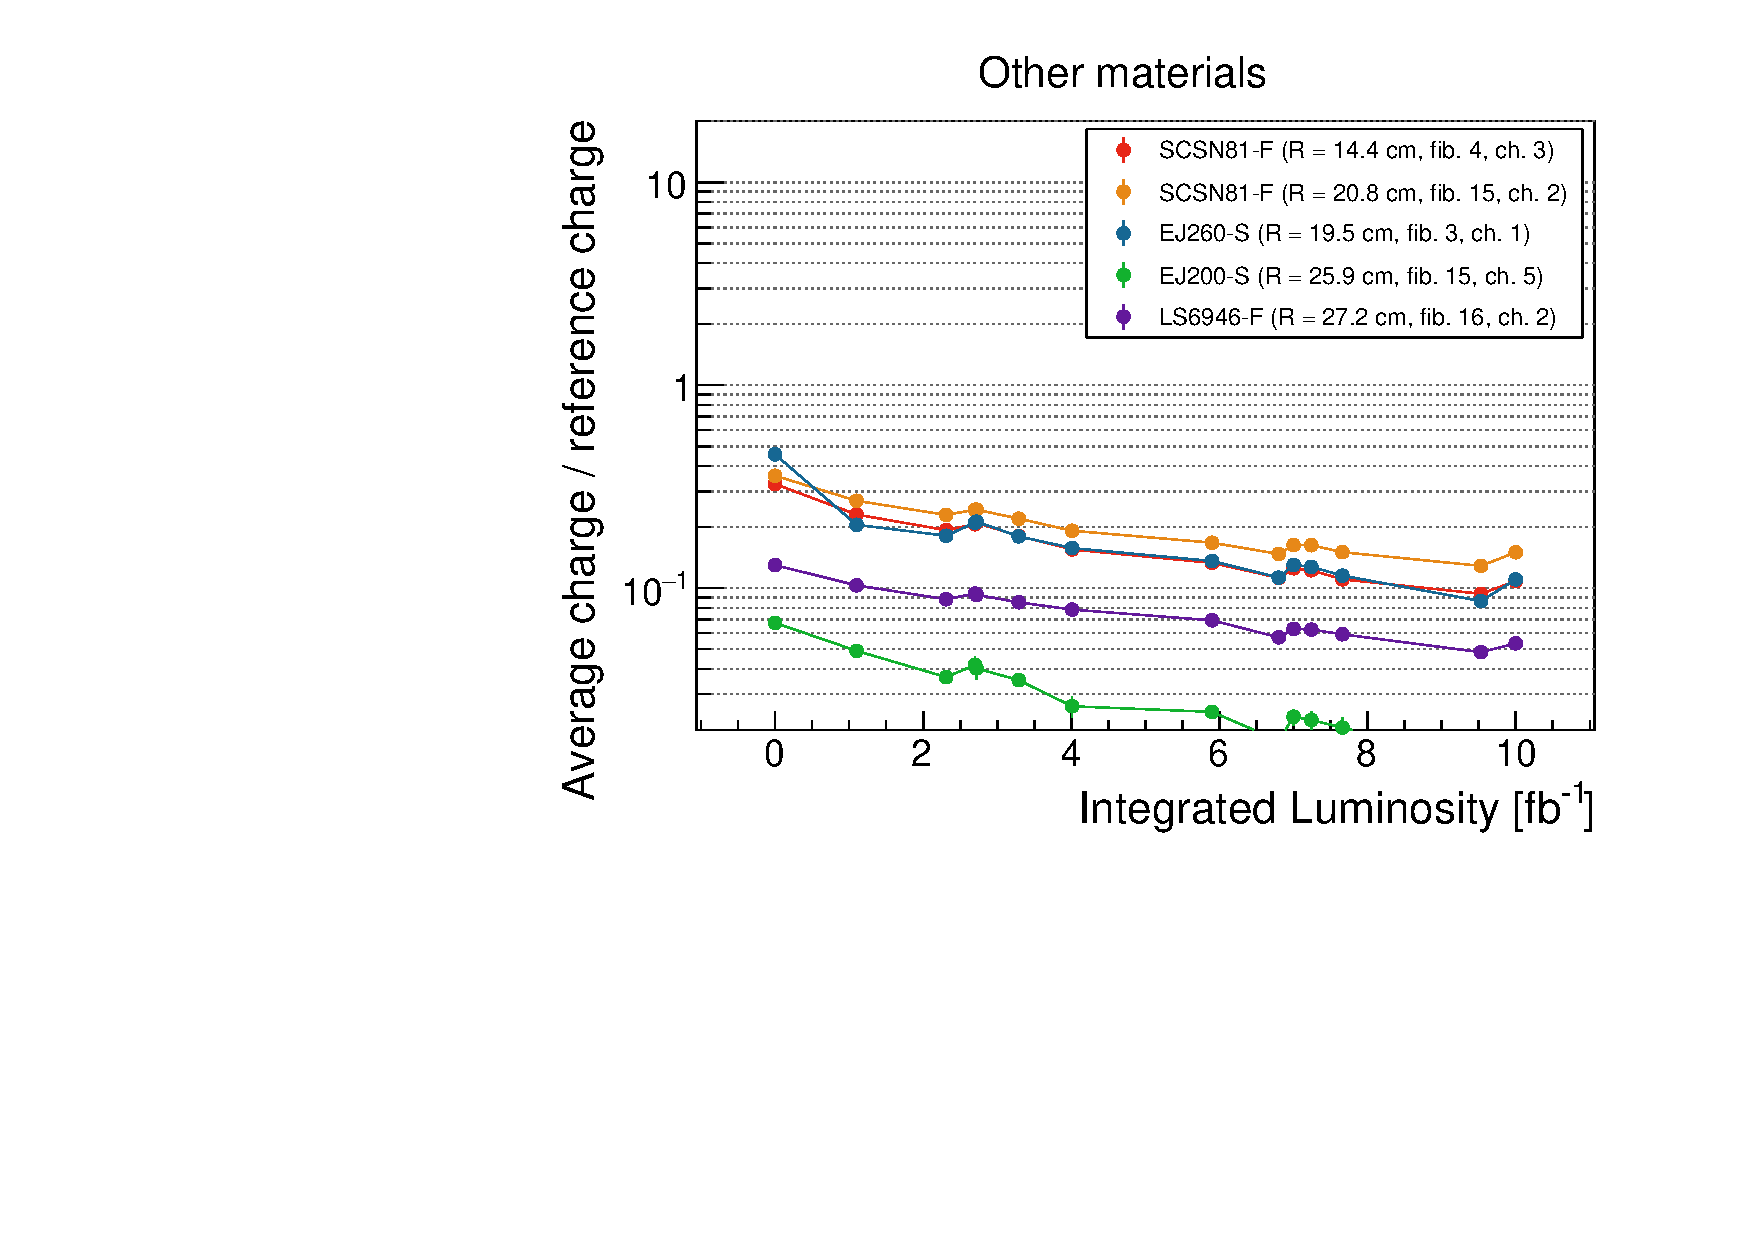
\includegraphics[width=0.46\textwidth]{figures/analysis/log_energy_lasercons_v14__bright_variety_vs_lumi_norm.pdf}
%\caption{Progression of average laser response normalized to the reference tile, as a function of delivered luminosity. Left: SCSN81-S tiles. Right: variety of alternative tiles. Variation due to laser amplitude is removed.}
%\label{energy_norm}
%\end{figure} 

%\begin{figure}[tbp!]
%\centering
%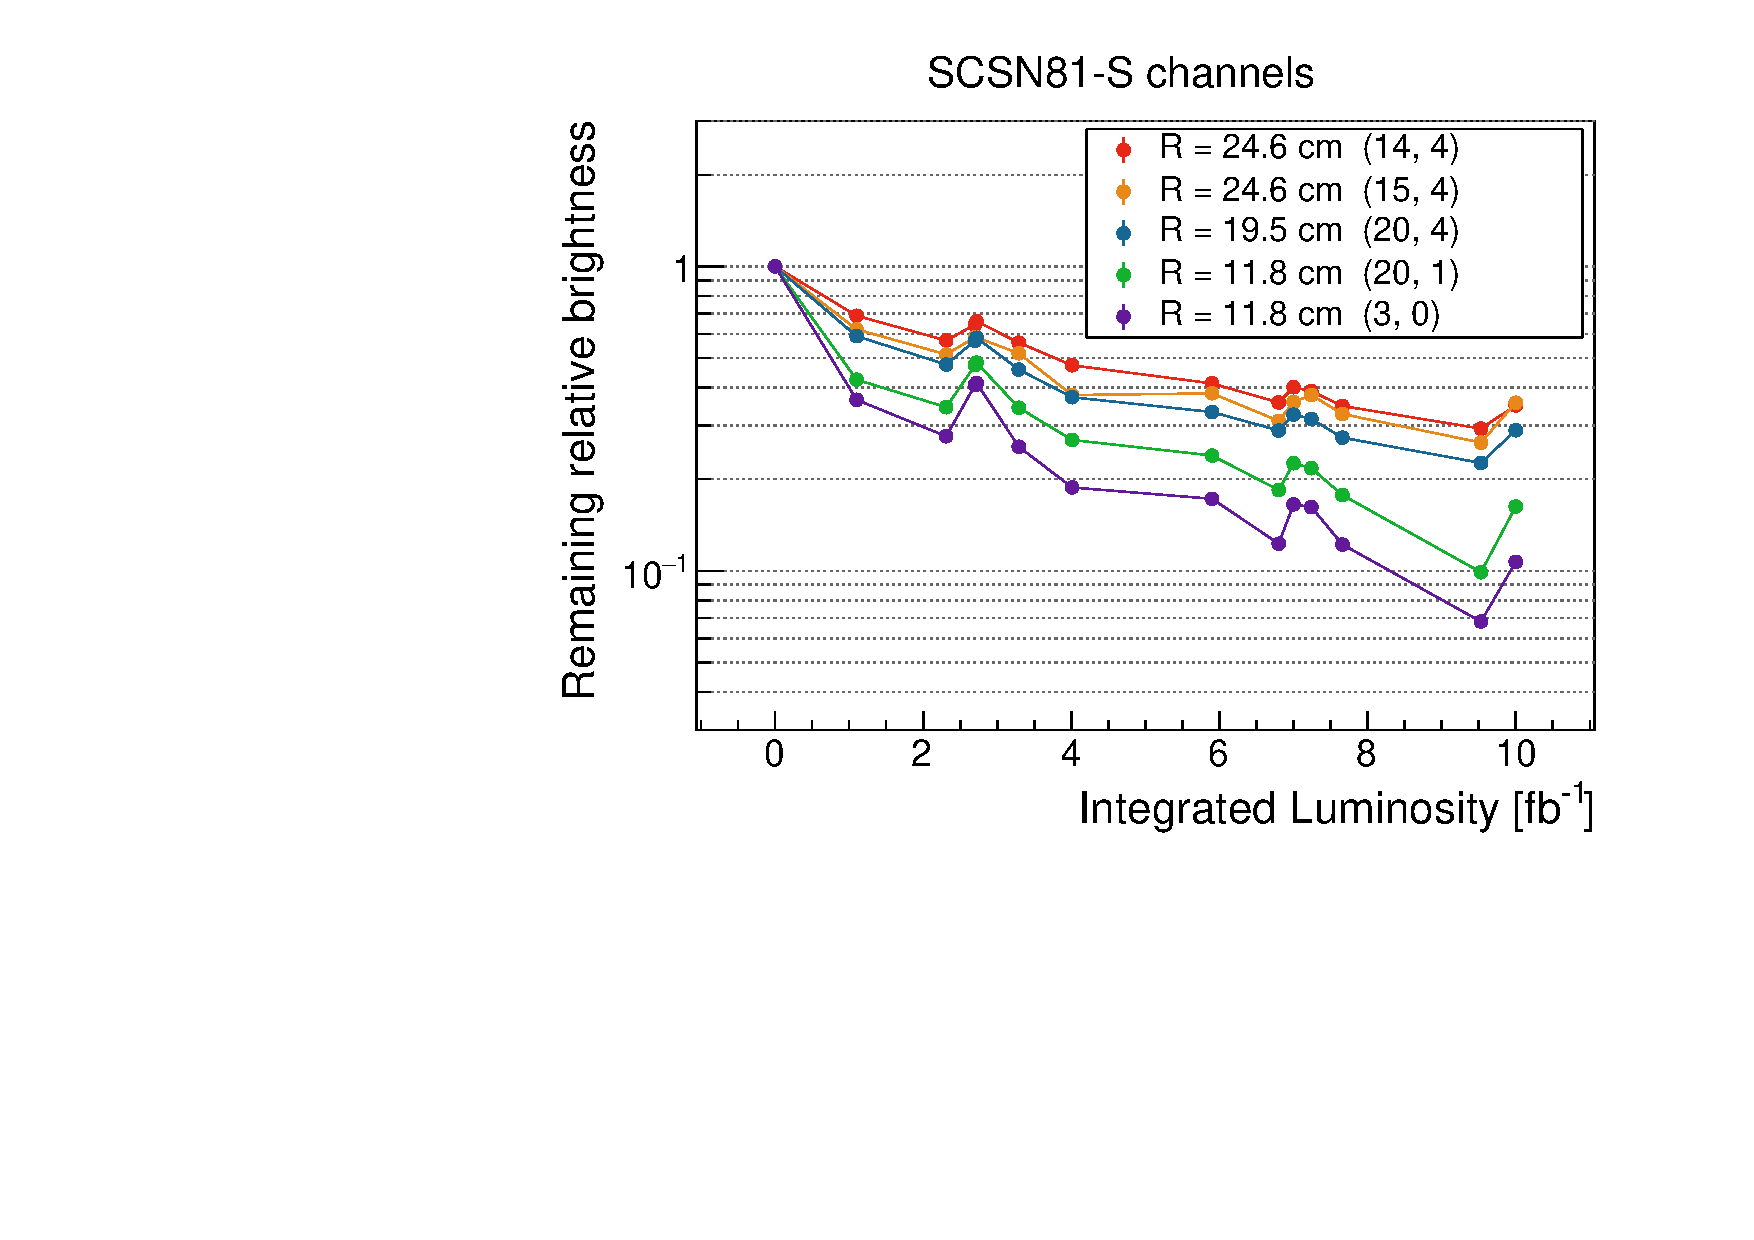
\includegraphics[width=0.46\textwidth]{figures/analysis/log_energy_lasercons_v14__scsnvar_vs_lumi_relative_change.pdf}
%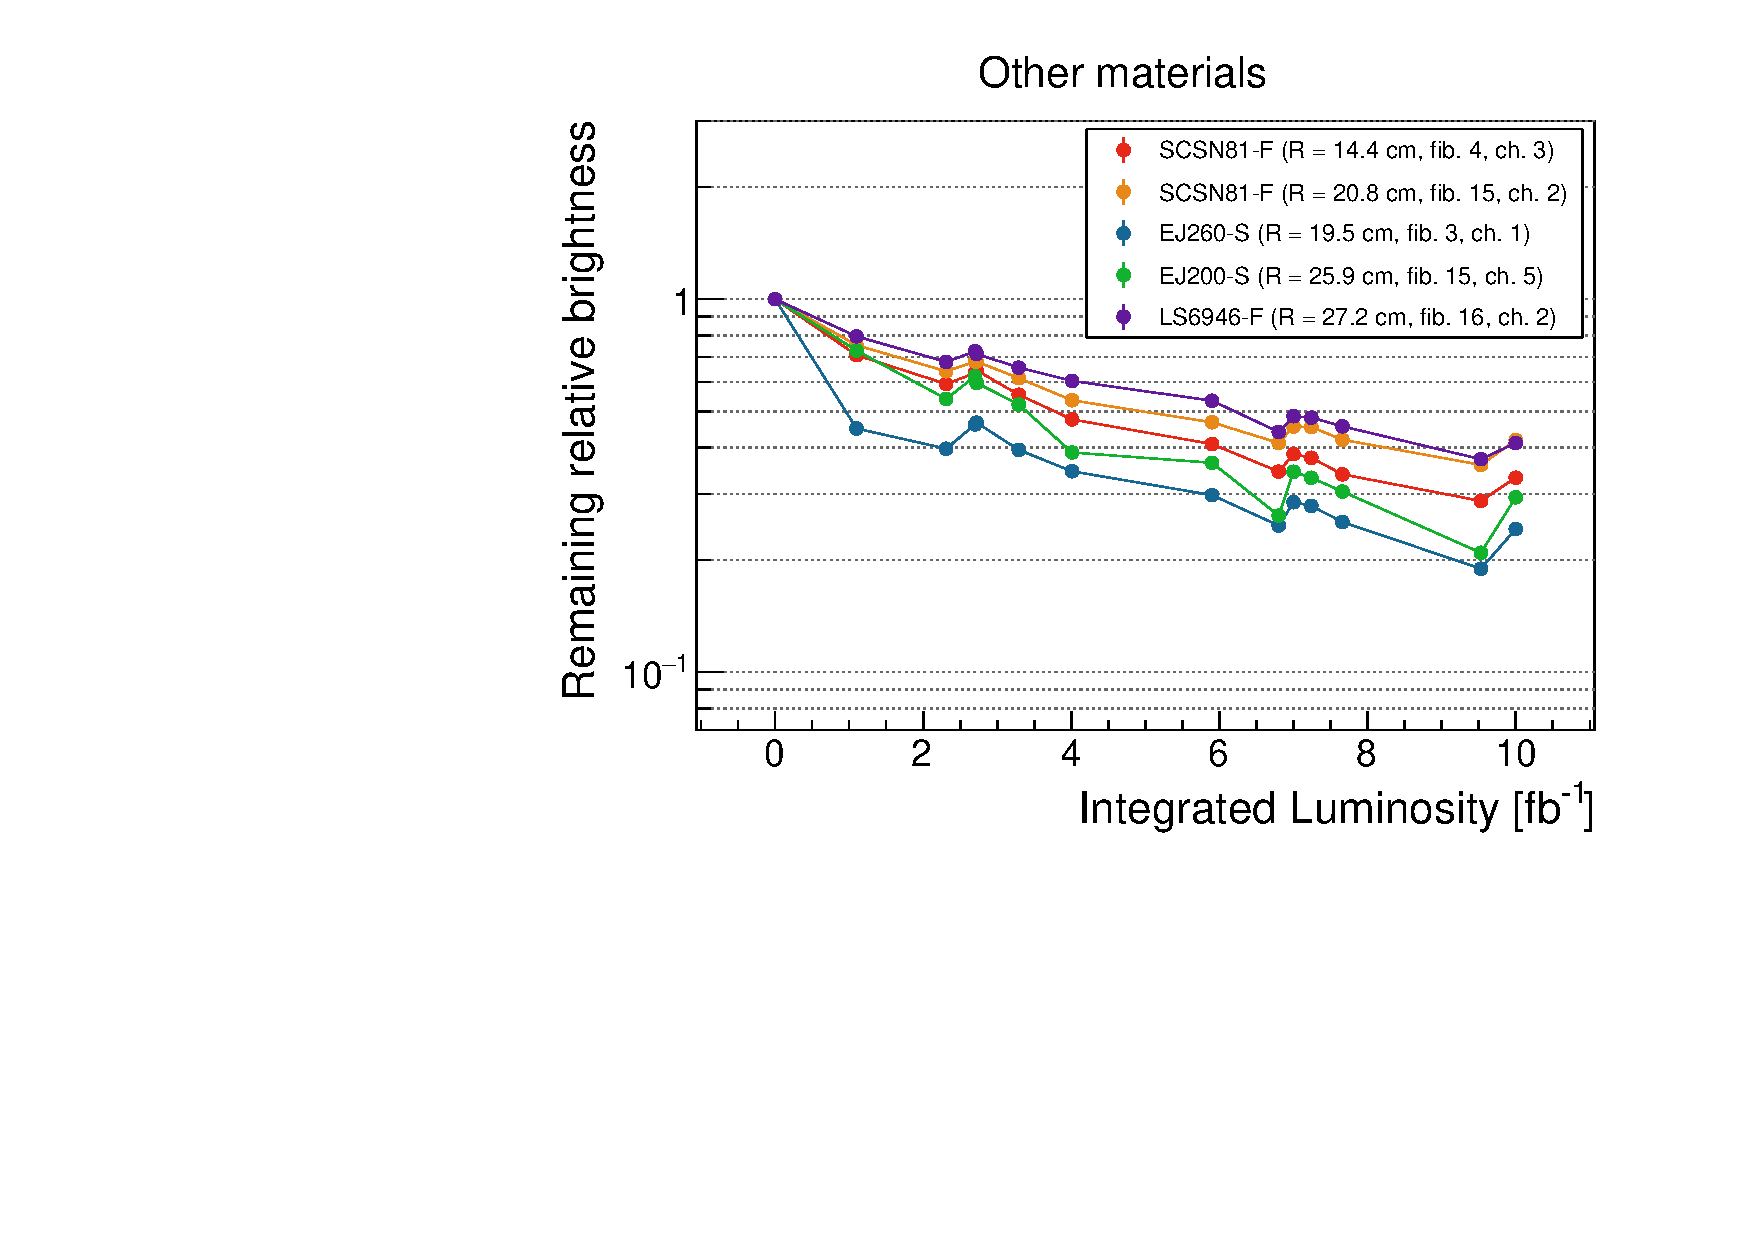
\includegraphics[width=0.46\textwidth]{figures/analysis/log_energy_lasercons_v14__bright_variety_vs_lumi_relative_change.pdf}
%\caption{Remaining laser response normalized to the initial response in each channel and to the reference tile response at each lumin%osity, as a function of delivered luminosity. Left: SCSN81-S tiles. Right: variety of alternative tiles.}
%\label{remaining_relative}
%\end{figure} 

%\begin{figure}[tbp!]
%\centering
%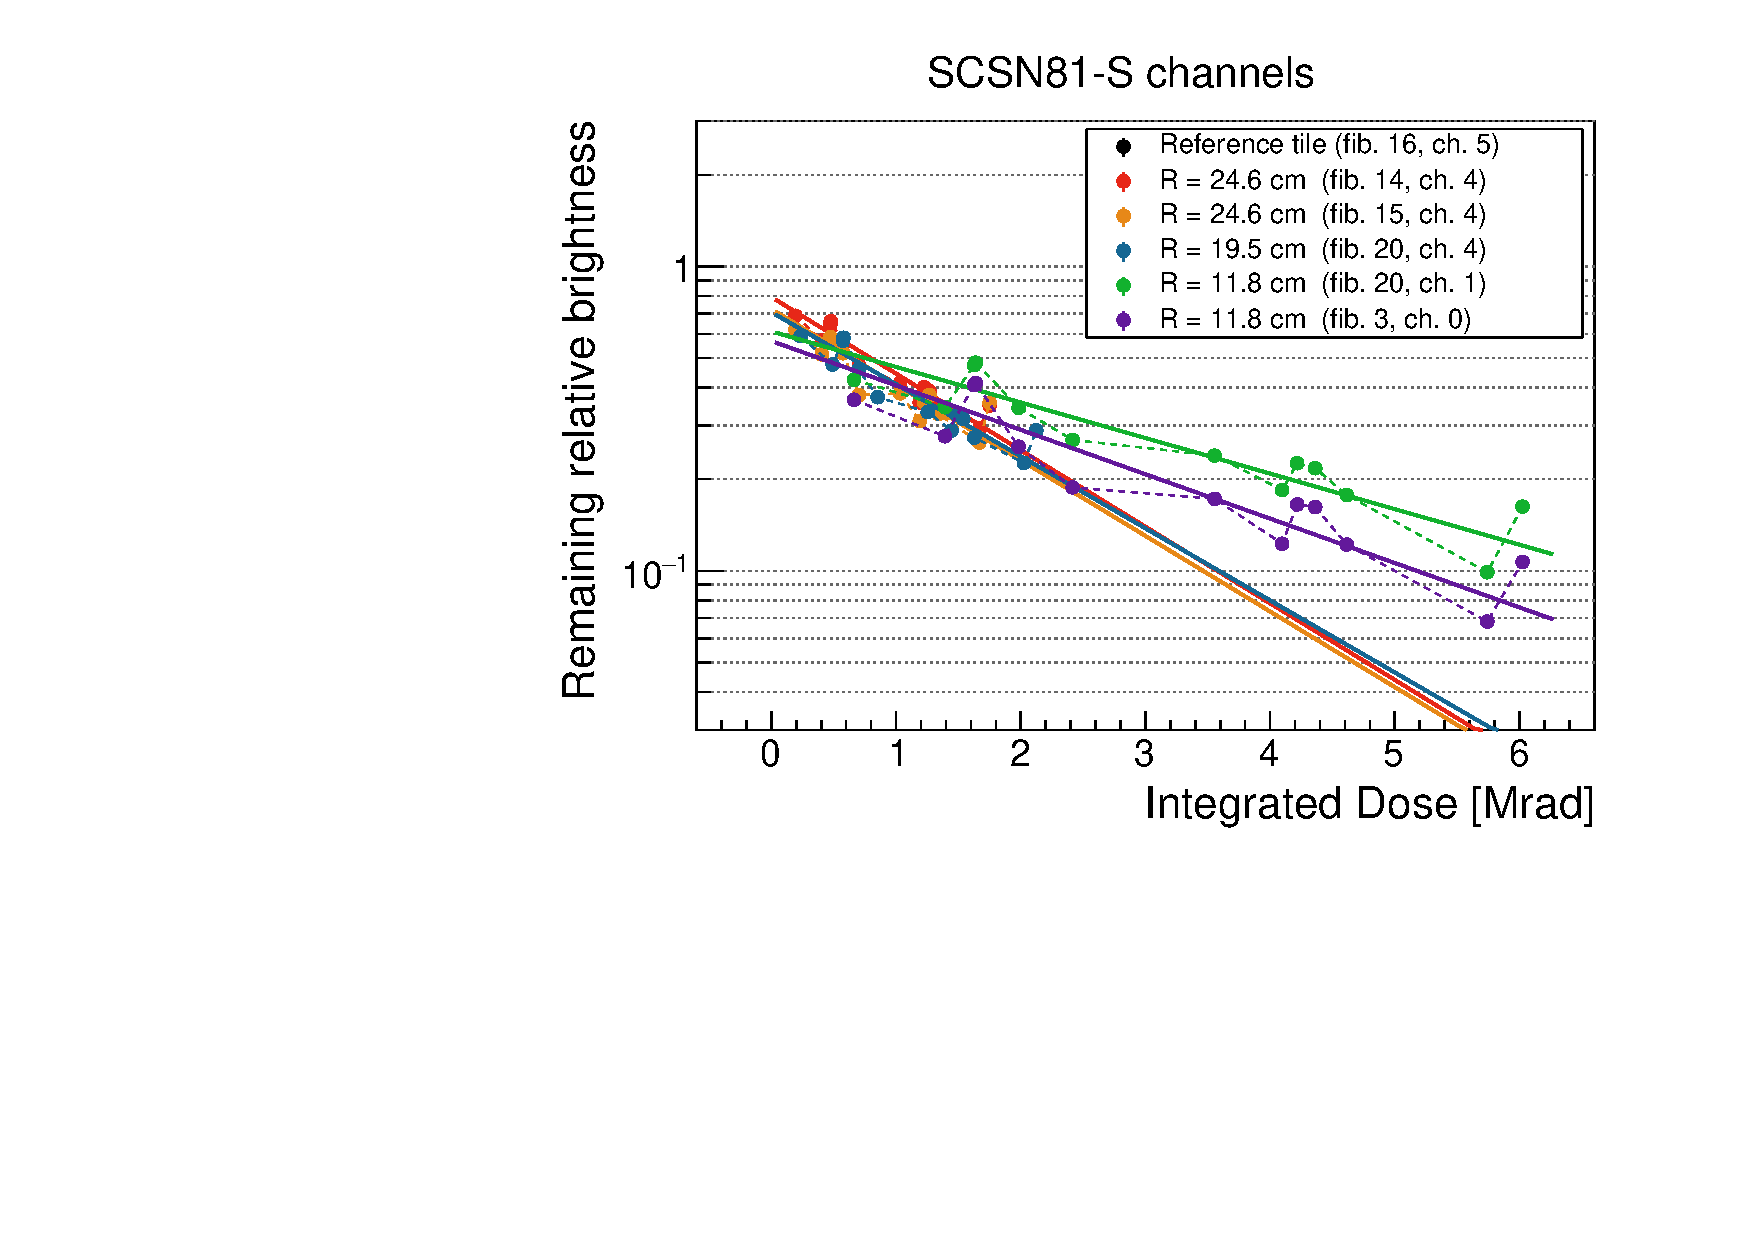
\includegraphics[width=0.46\textwidth]{figures/analysis/log_energy_lasercons_v14__scsnvar_vs_dose_relative_change.pdf}
%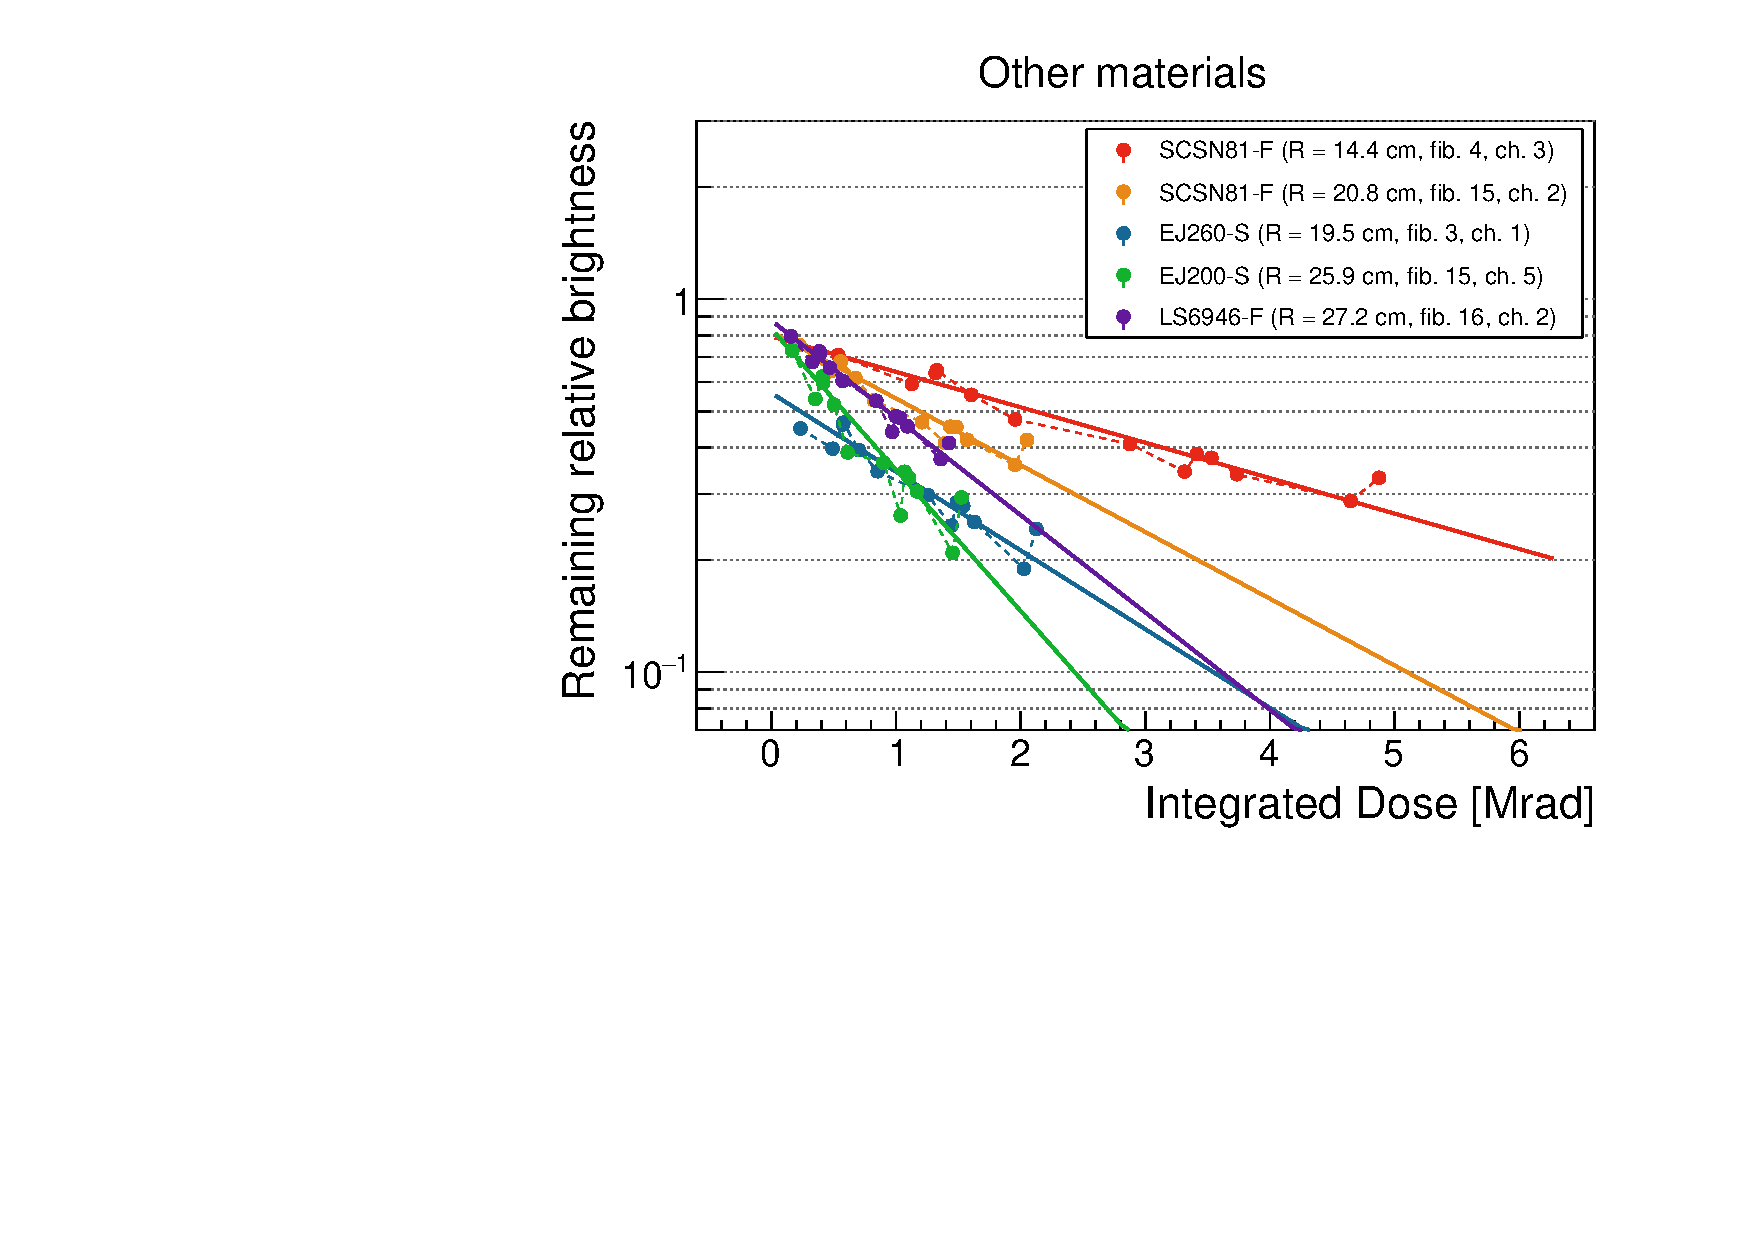
\includegraphics[width=0.46\textwidth]{figures/analysis/log_energy_lasercons_v14__bright_variety_vs_dose_relative_change.pdf}
%\caption{Remaining laser response as a function of received dose, normalized to the initial response in each channel and to the reference tile response at each measurement. Left: SCSN81-S tiles. Right: variety of alternative tiles. The slope of the remaining light yield indicates the dose constant. Shallower slopes (larger dose constants) are expected for tiles with greater irradiation due to dose rate effects.}
%\label{remaining_relative_dose}
%\end{figure} 


\subsection{Systematic uncertainties\label{sec:ana-unc}}

There are unknown and unmeasurable systematics at play in the experimental setup, including variation in the quality of the optical connection between laser and tiles after the laser splitting, unknown amounts of radiation damage to the reference tile used for normalization, and an unexplained steep drop in relative light yield for all tiles during the initial phase of irradiation, followed by a slower, steady-state exponential decay.

The light yield curve also shows a significant amount of recovery in the post-collisions period when there was no irradiation. The dose constants measured in this paper are measured after the temporary damage in the tiles has annealed and only the permanent damage remains. However, the day-0 light yield cannot be used as the pre-irradiation value for the steady-state exponential decay because the initial stage of the damage mechanism is characterized by the steeper rate of light loss that is not yet understood. Therefore, the L(0) value used in the calculation of the post-recovery dose constant is found by fitting an exponential curve to the L(\textit{d})/L(0) points as a function of integrated dose only during the steady-state exponential decay region, extrapolating the curve to a dose of 0 Mrad, and taking the dose = 0 intercept as L(0) in Equation~\ref{eq:lightloss}. The equation is then solved for the dose constant D.

The statistical uncertainty on each L(\textit{d})/L(0) measurement is calculated via error propagation from the RMS's of the light yield distributions of the signal and reference tiles at dose \textit{d} and on day 0.

All in all, the light yield curve exhibits variations larger than the statistical uncertainty, due to an ensemble of systematics including the steep drop in the initial state of irradiation and also run-to-run variation in light transmission from tile to readout module. To cover this, a conservative systematic uncertainty of 20\% is added in quadrature to the statistical uncertainty to yield the total uncertainty.

\subsection{Results\label{sec:ana-res}}

\subsubsection{Light yield versus dose\label{sec:ana-res-lyvsdose}}

The relative light yields for the various tiles as a function of total received dose are shown here in Figures~\ref{fig:SCSN81-S-11p8cm-dose} to~\ref{fig:EJ260-F-dose}. Each plot shows also the fitted exponential curve to the steady-state exponential decay, which is used to extrapolate to zero dose to get the initial light yield used to solve for the dose constant after recovery.

\begin{figure}[tbp!]
\centering
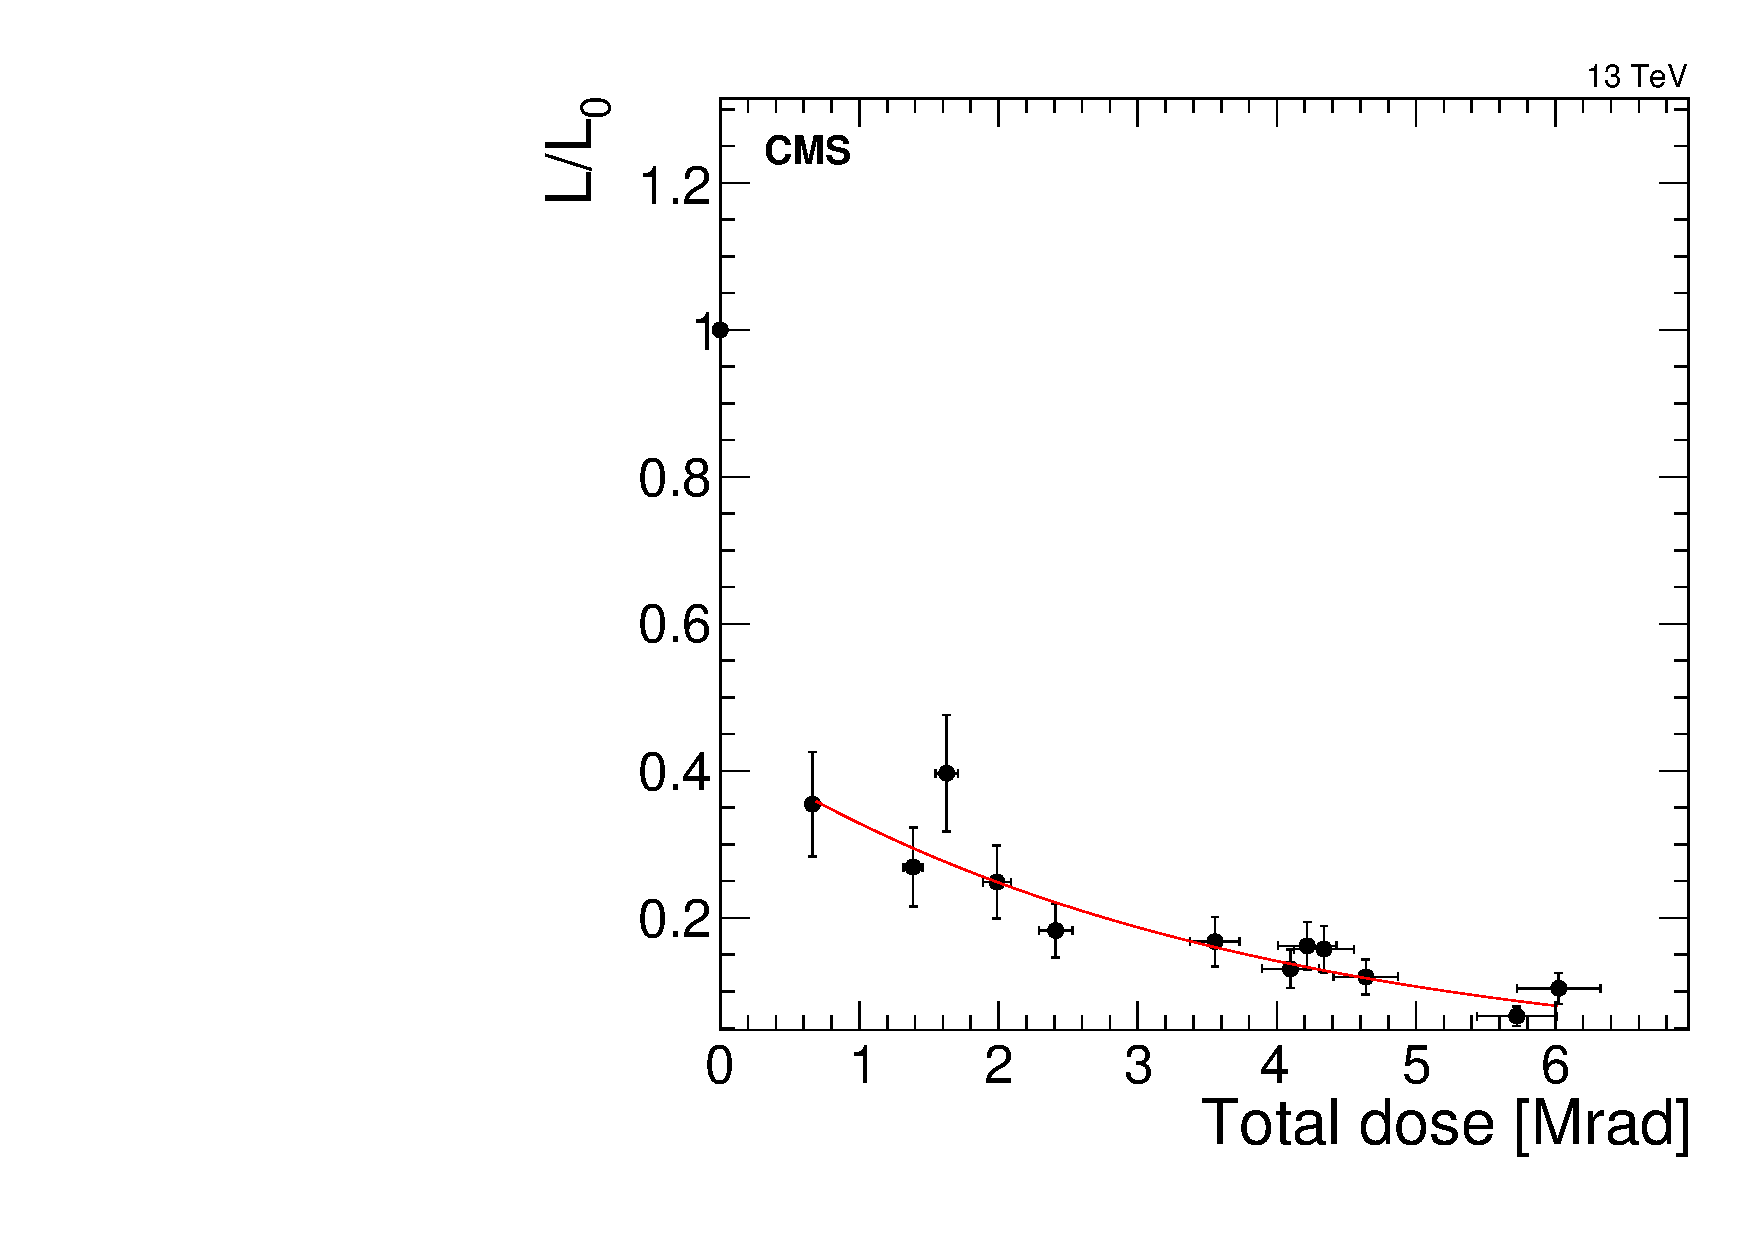
\includegraphics[width=0.45\textwidth]{figures/SCSN81-S-11p8cm-f3ch0-dose.pdf}
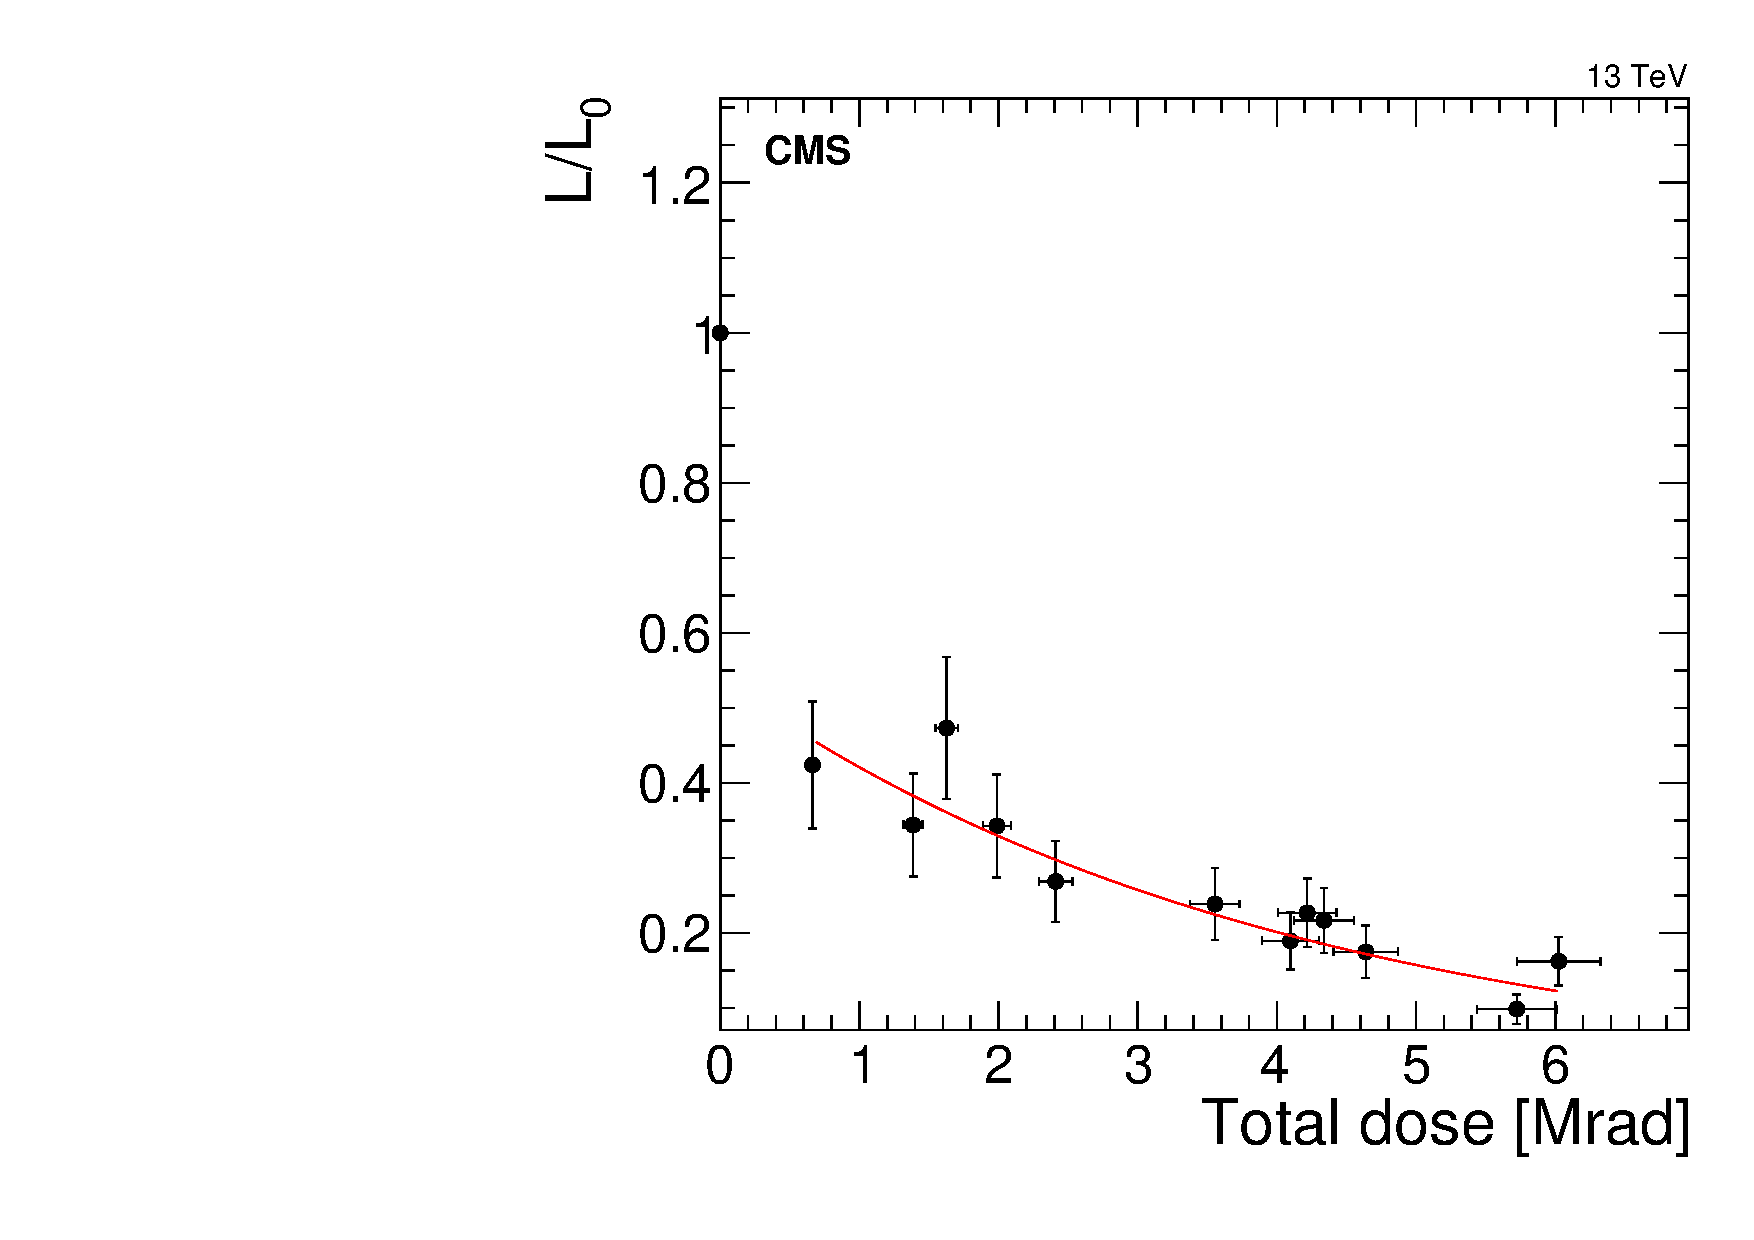
\includegraphics[width=0.45\textwidth]{figures/SCSN81-S-11p8cm-f20ch1-dose.pdf}
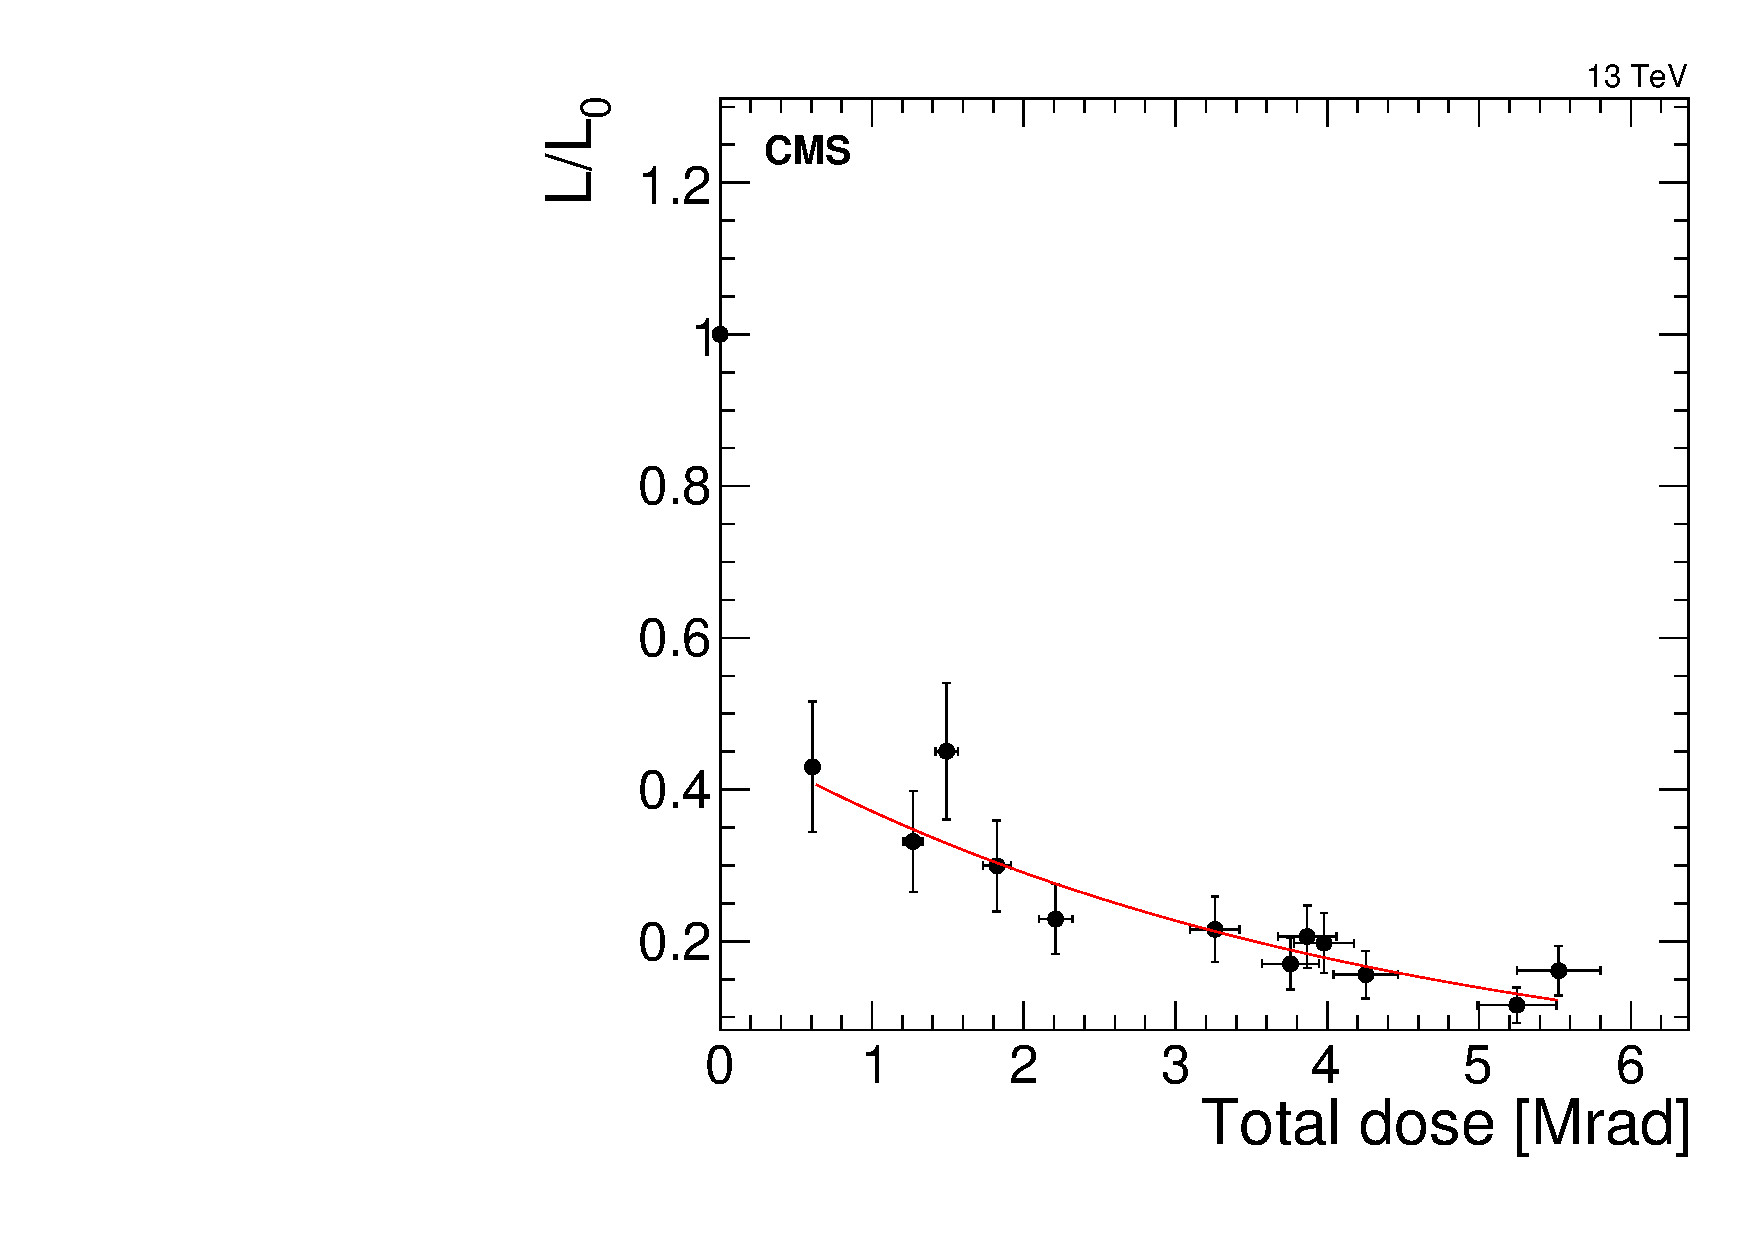
\includegraphics[width=0.45\textwidth]{figures/SCSN81-S-13p1cm-f7ch5-dose.pdf}
\caption{Relative yield versus integrated dose for SCSN81 sigma tiles at 11.8 cm (top left and right) and 13.1 cm (bottom) from the CMS beam pipe, receiving 16.61 krad/hr and 15.23 krad/hr respectively. The exponential decay curve fitted to the steady-state region of light loss is shown in red.}
\label{fig:SCSN81-S-11p8cm-dose}
\end{figure} 

\begin{figure}[tbp!]
\centering
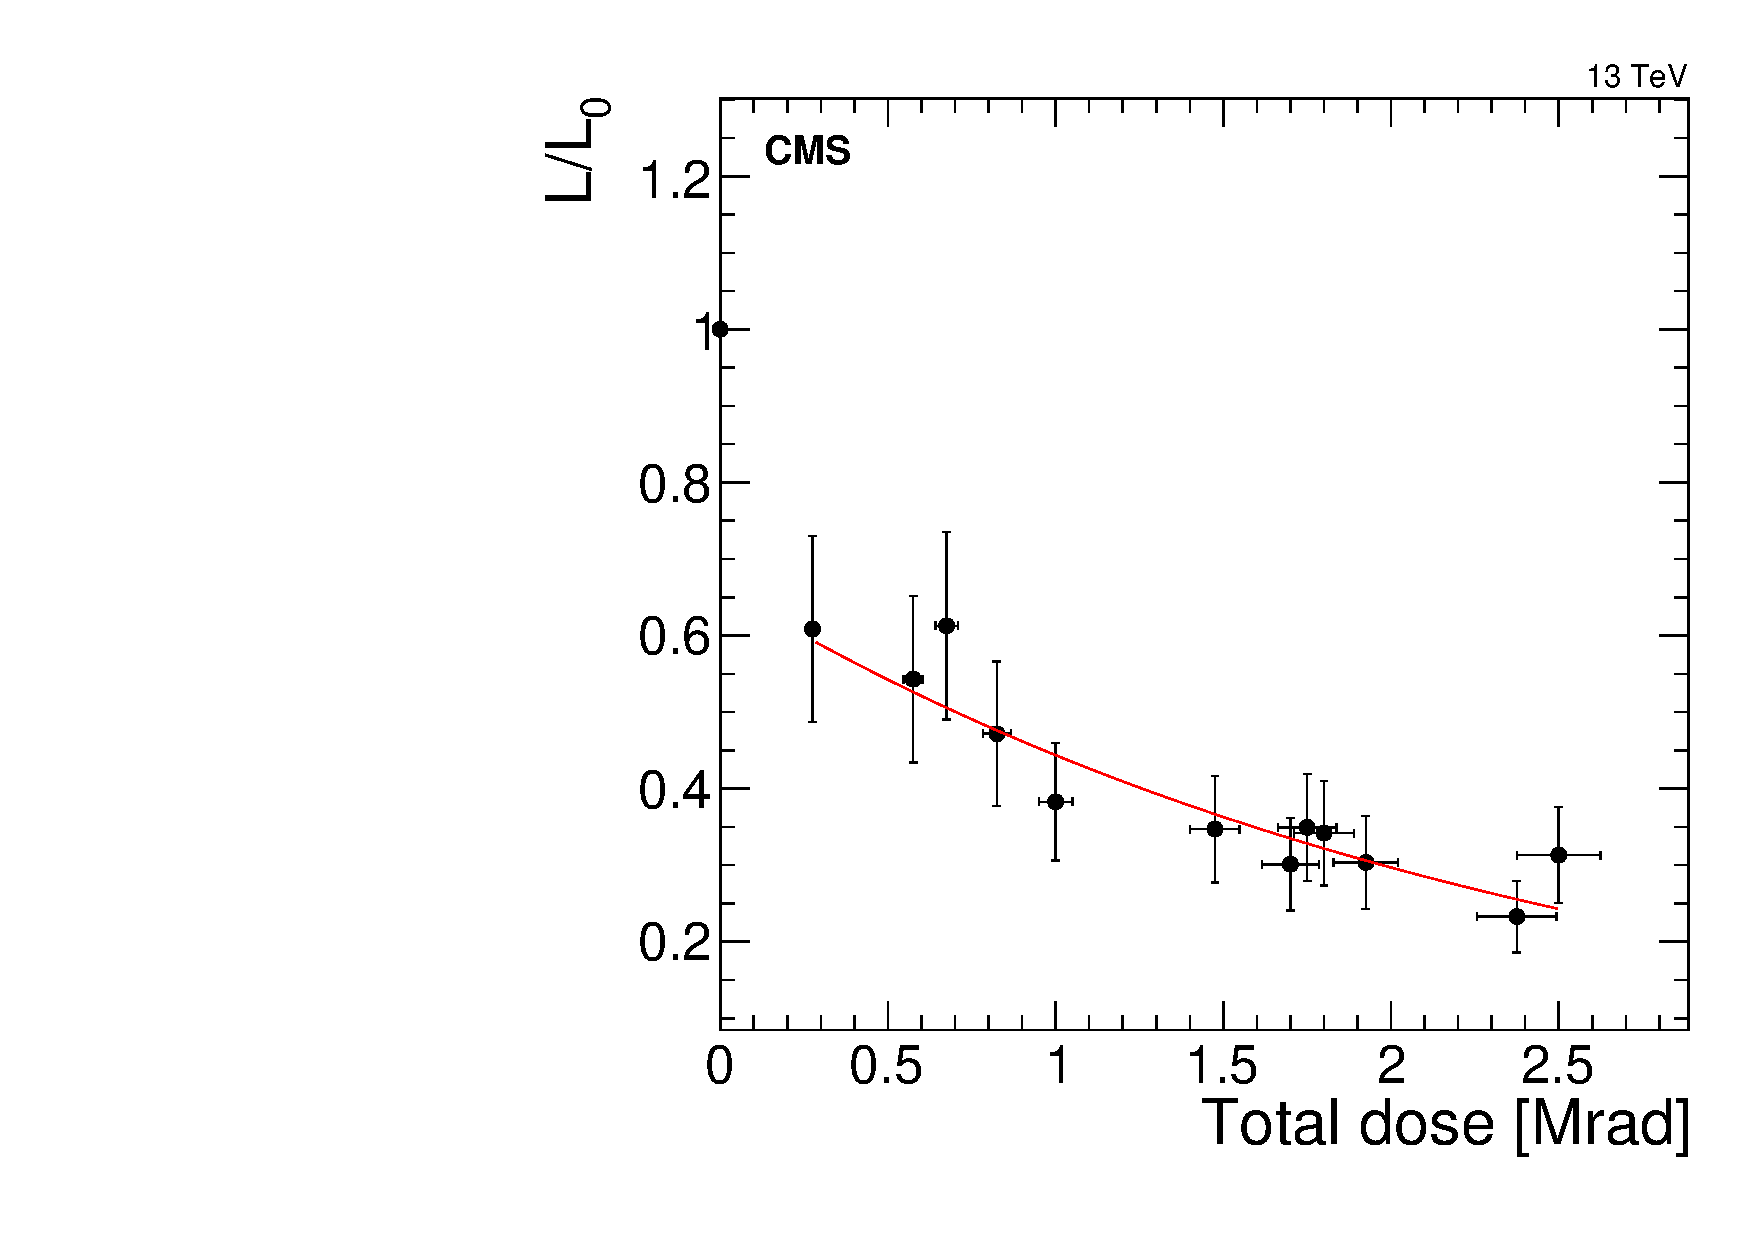
\includegraphics[width=0.45\textwidth]{figures/SCSN81-S-18p2cm-f5ch0-dose.pdf}
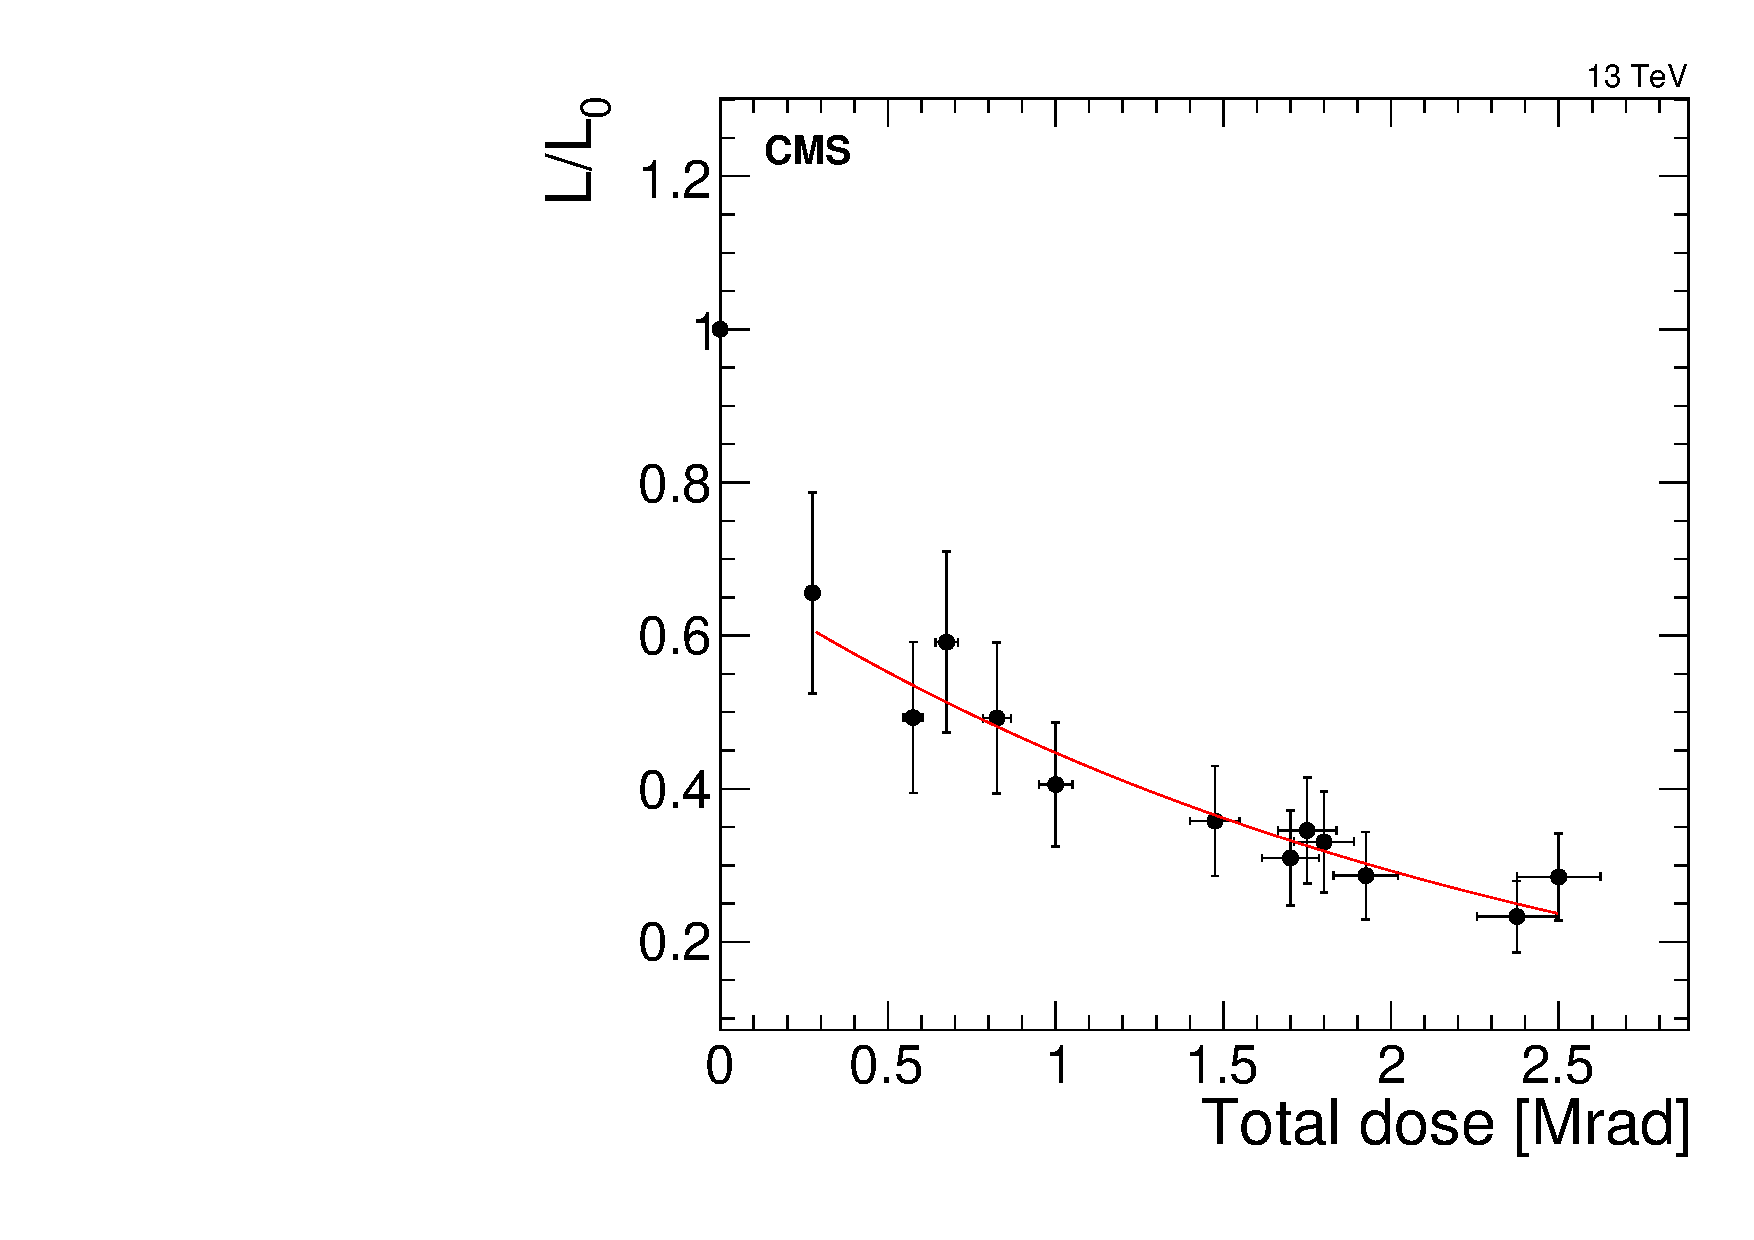
\includegraphics[width=0.45\textwidth]{figures/SCSN81-S-18p2cm-f20ch5-dose.pdf}
\caption{Relative yield versus integrated dose for SCSN81 sigma tiles at 18.2 cm from the CMS beam pipe, receiving 6.89 krad/hr. The exponential decay curve fitted to the steady-state region of light loss is shown in red.}
\label{fig:SCSN81-S-18p2cm-dose}
\end{figure} 

\begin{figure}[tbp!]
\centering
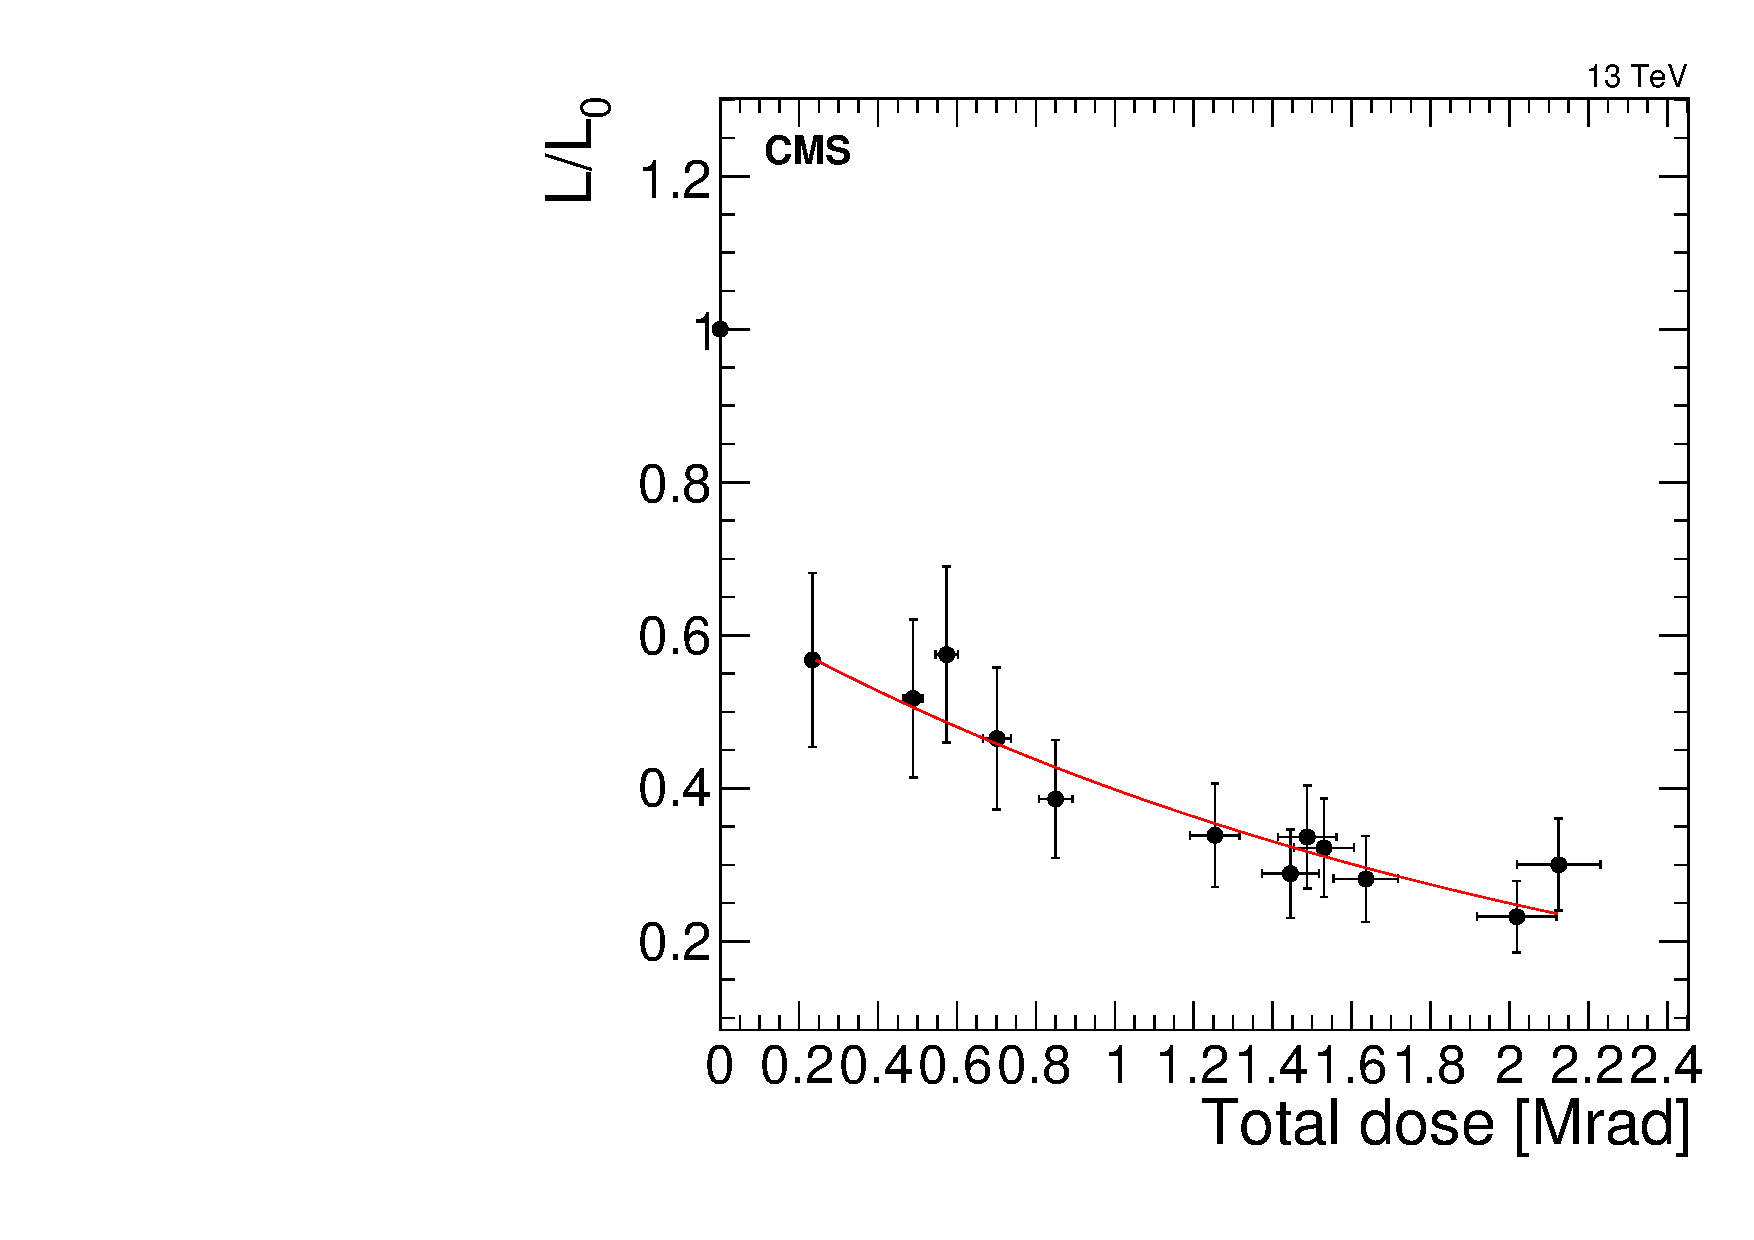
\includegraphics[width=0.45\textwidth]{figures/SCSN81-S-19p5cm-f2ch1-dose.pdf}
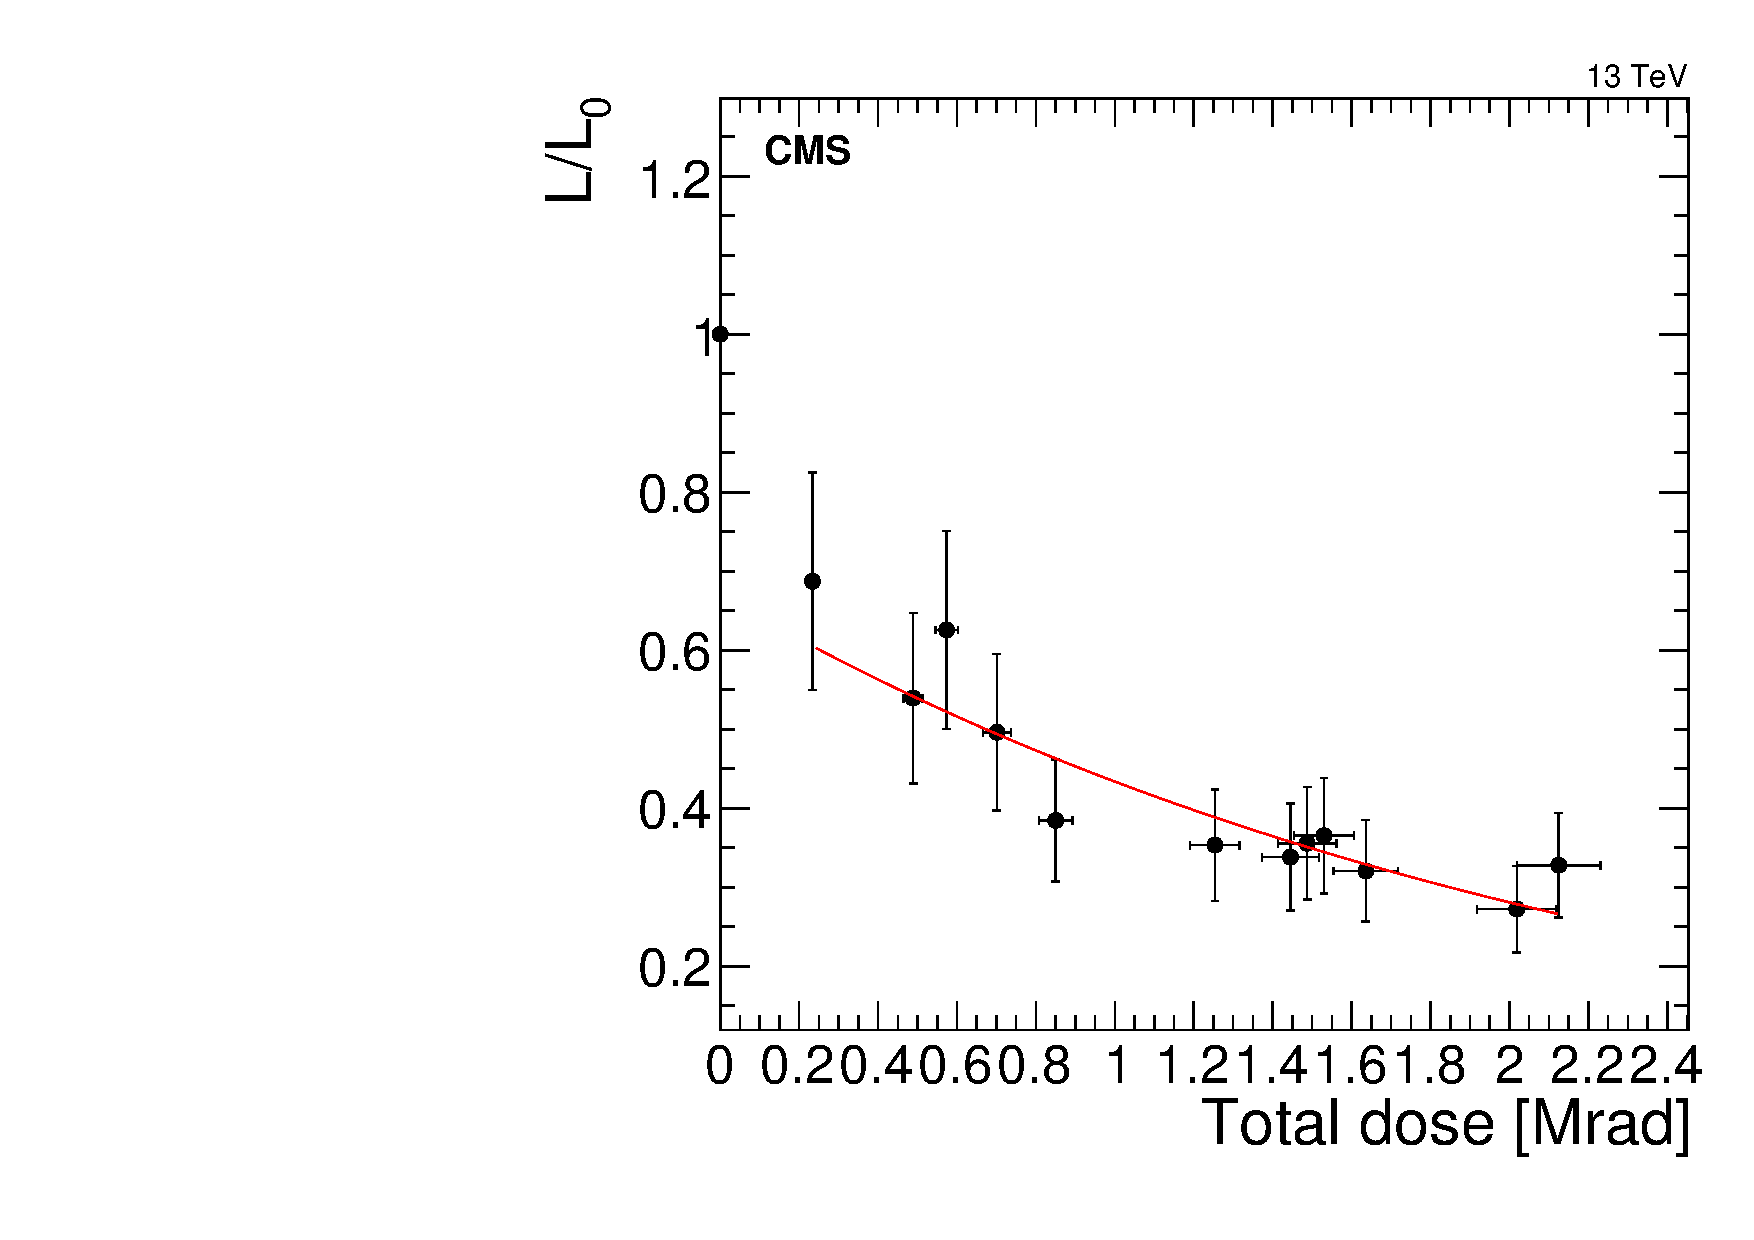
\includegraphics[width=0.45\textwidth]{figures/SCSN81-S-19p5cm-f15ch1-dose.pdf}
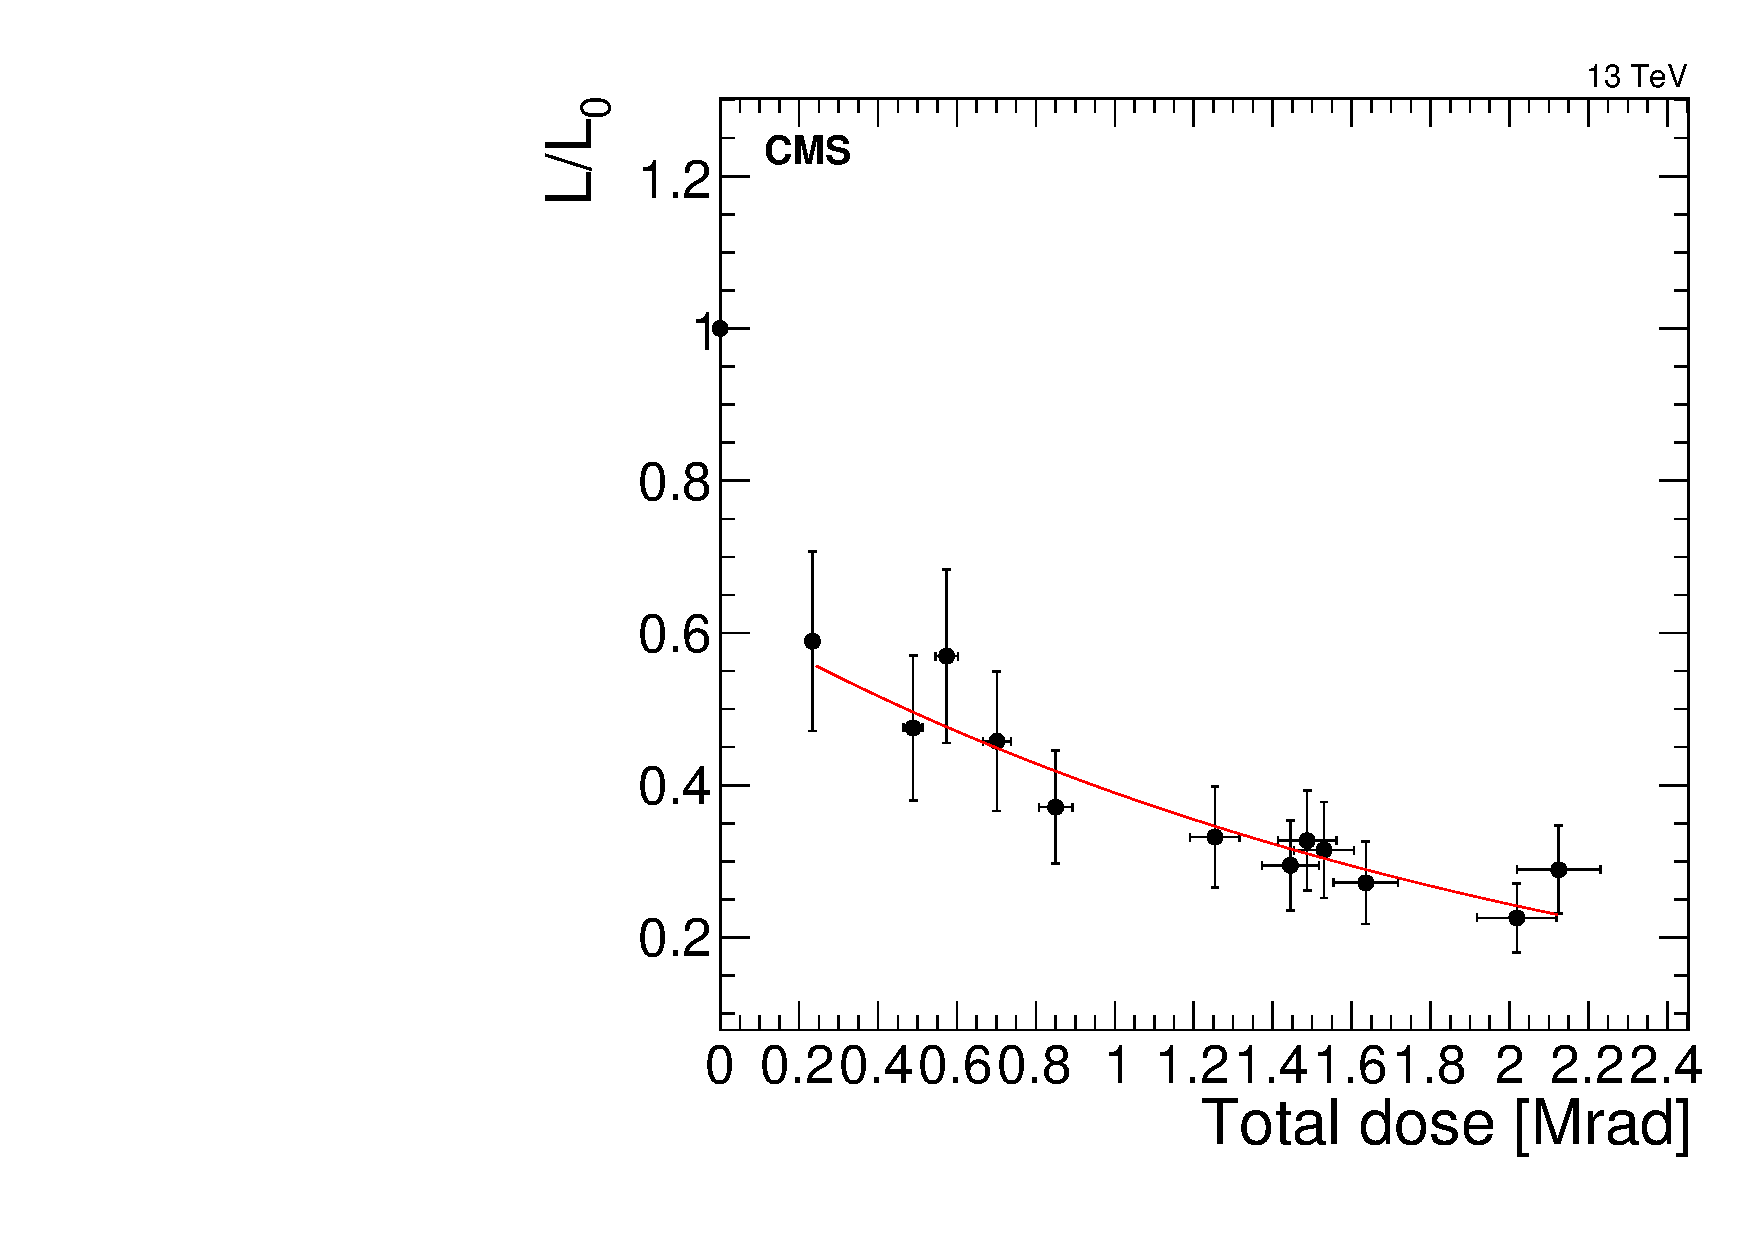
\includegraphics[width=0.45\textwidth]{figures/SCSN81-S-19p5cm-f20ch4-dose.pdf}
\caption{Relative yield versus integrated dose for SCSN81 sigma tiles at 19.5 cm from the CMS beam pipe, receiving 5.86 krad/hr. The exponential decay curve fitted to the steady-state region of light loss is shown in red.}
\label{fig:SCSN81-S-19p5cm-dose}
\end{figure} 

\begin{figure}[tbp!]
\centering
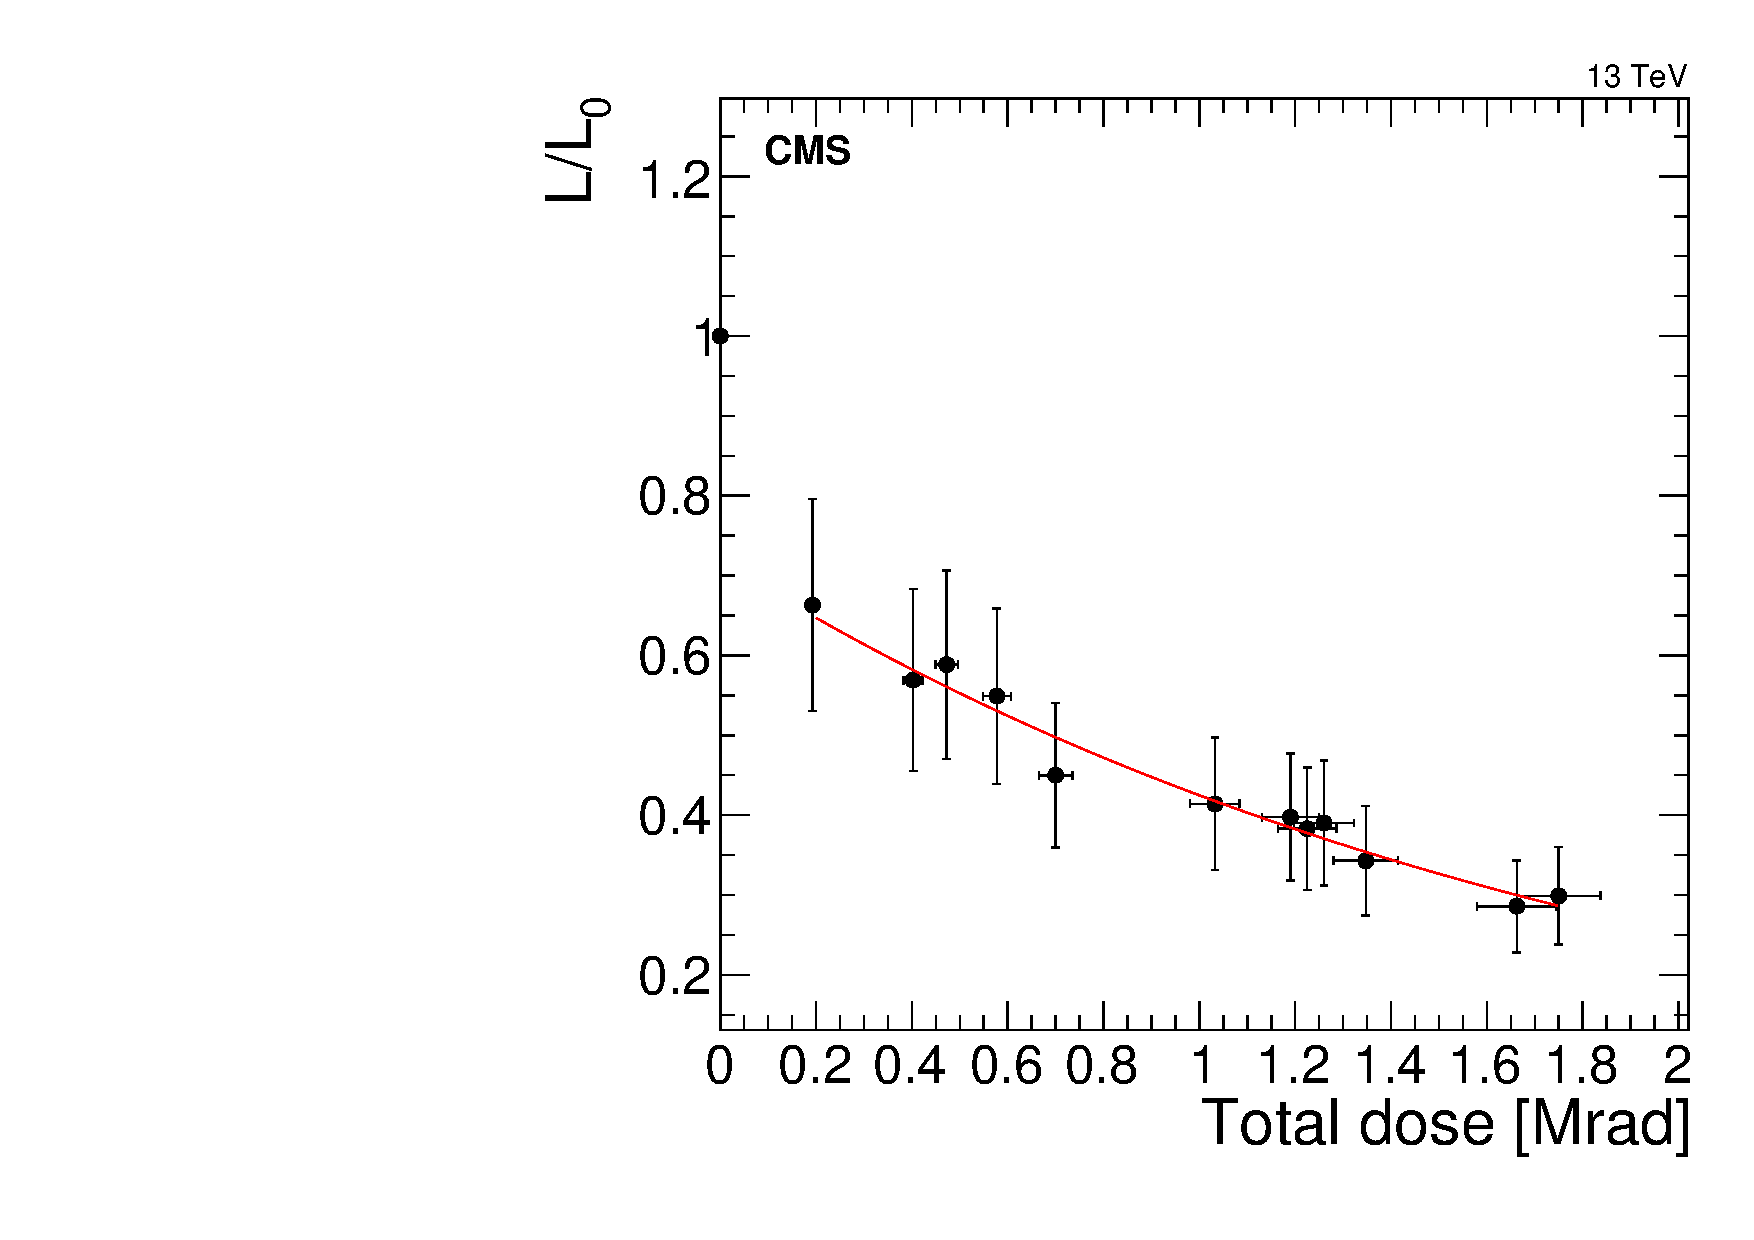
\includegraphics[width=0.45\textwidth]{figures/SCSN81-S-24p6cm-f3ch2-dose.pdf}
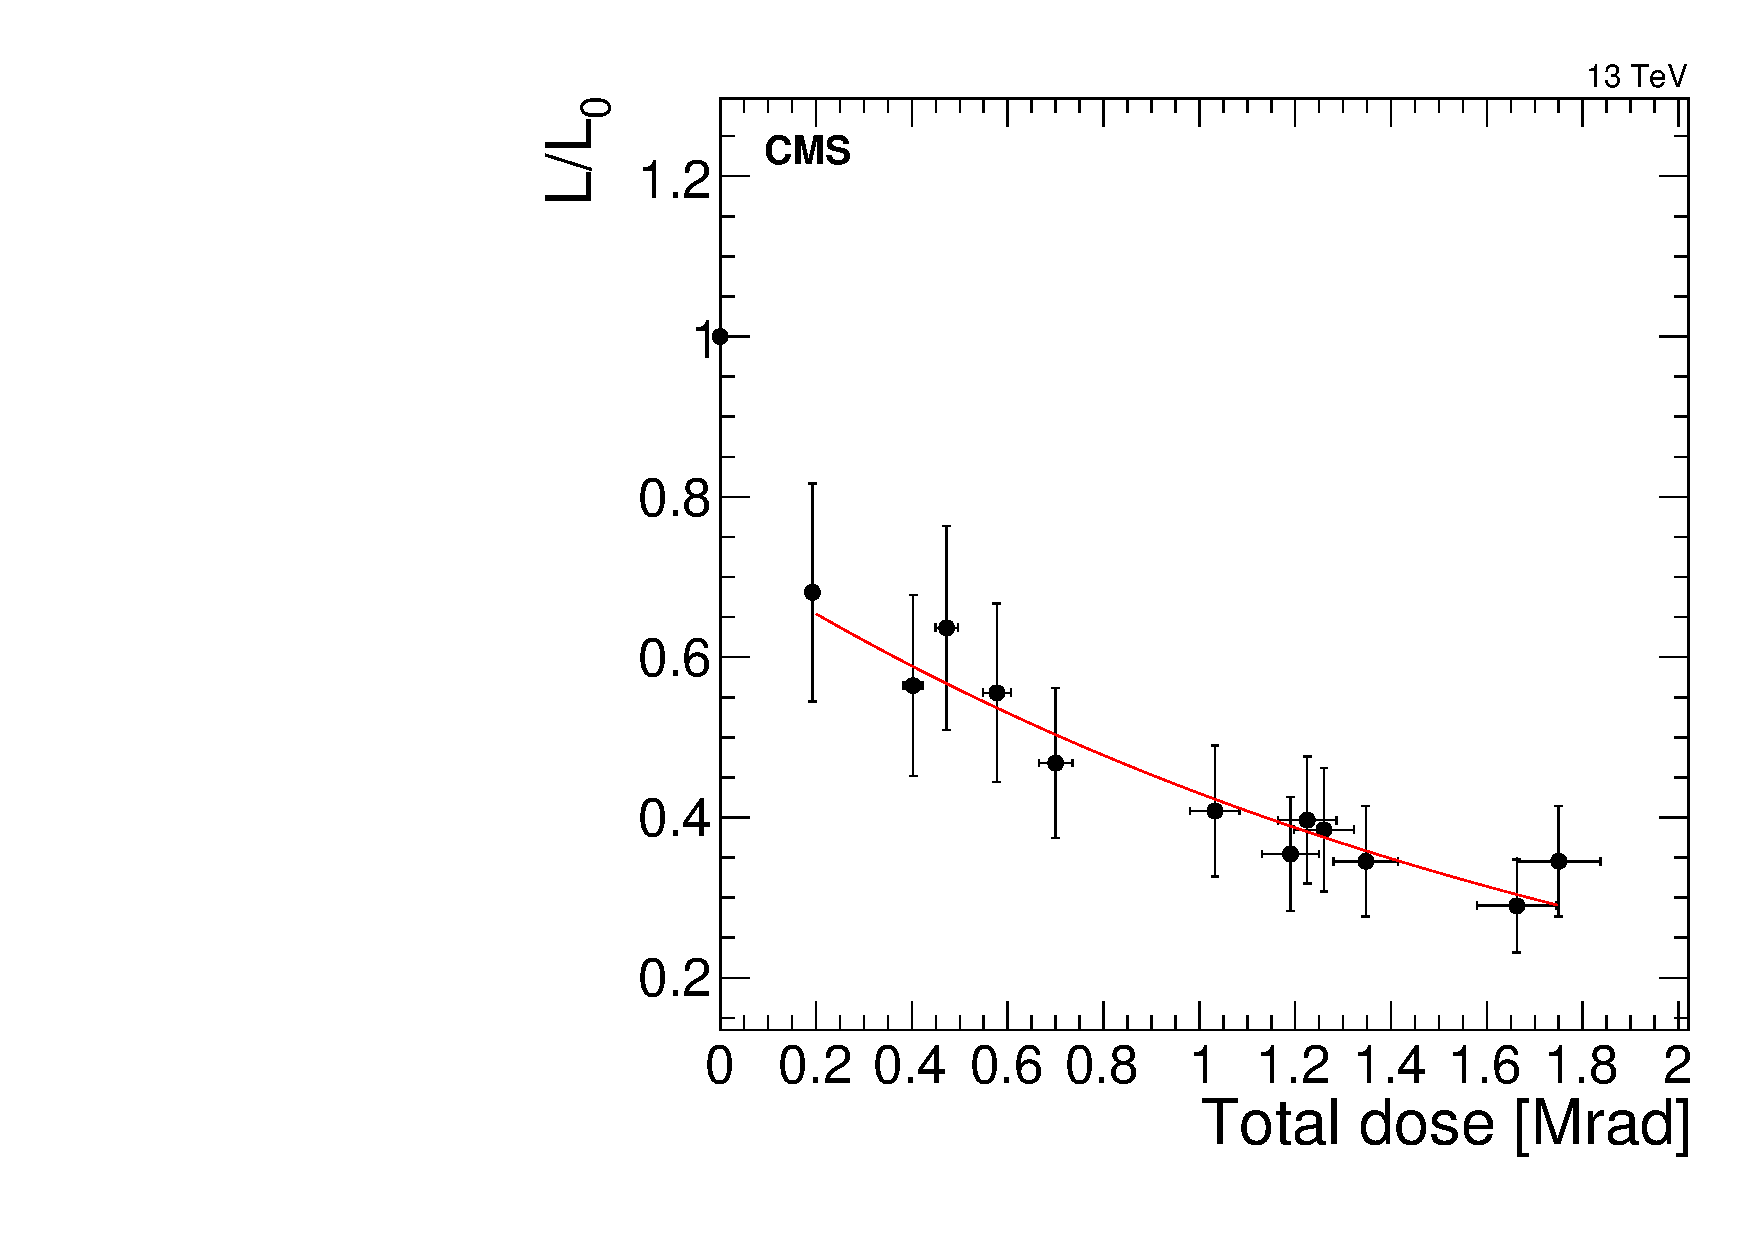
\includegraphics[width=0.45\textwidth]{figures/SCSN81-S-24p6cm-f14ch4-dose.pdf}
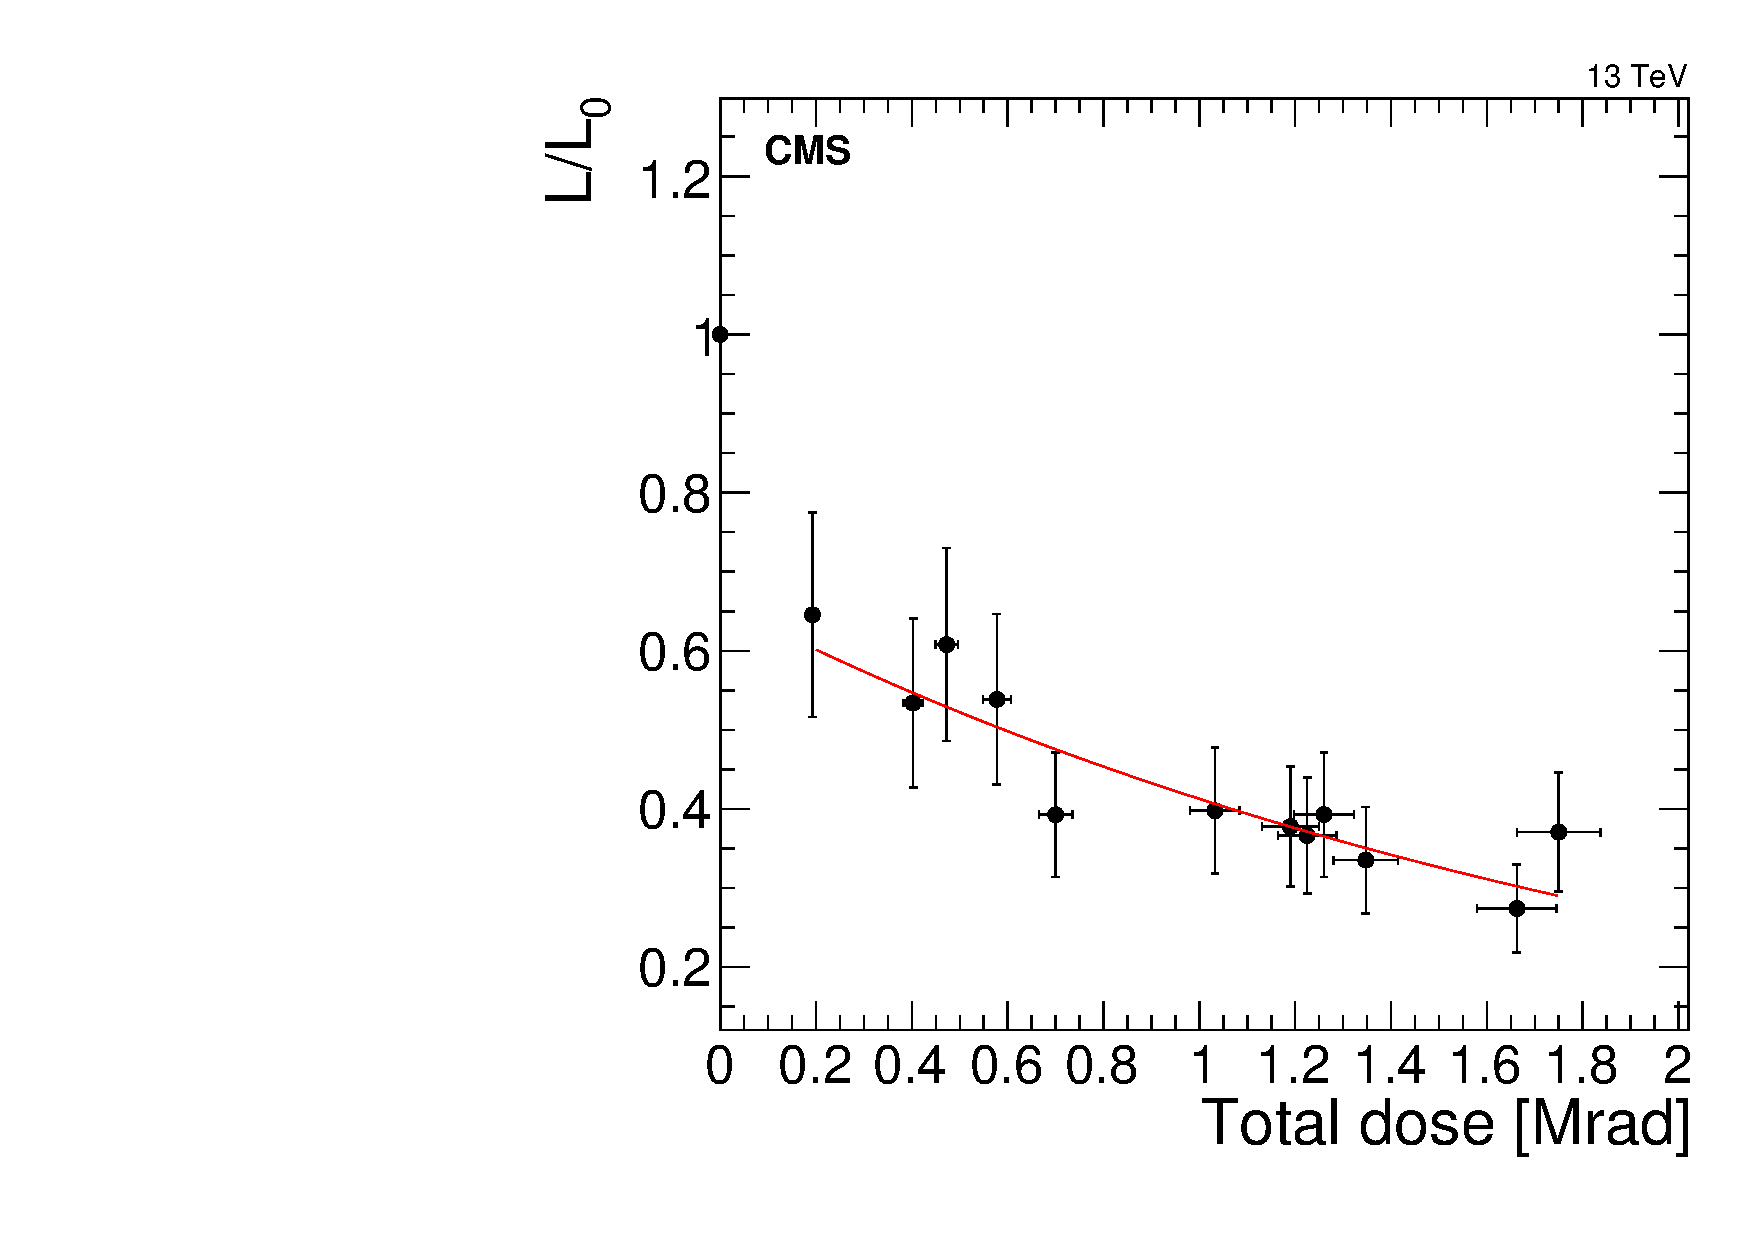
\includegraphics[width=0.45\textwidth]{figures/SCSN81-S-24p6cm-f15ch4-dose.pdf}
\caption{Relative yield versus integrated dose for SCSN81 sigma tiles at 24.6 cm from the CMS beam pipe, receiving 4.82 krad/hr. The exponential decay curve fitted to the steady-state region of light loss is shown in red.}
\label{fig:SCSN81-S-24p6cm-dose}
\end{figure} 

\begin{figure}[tbp!]
\centering
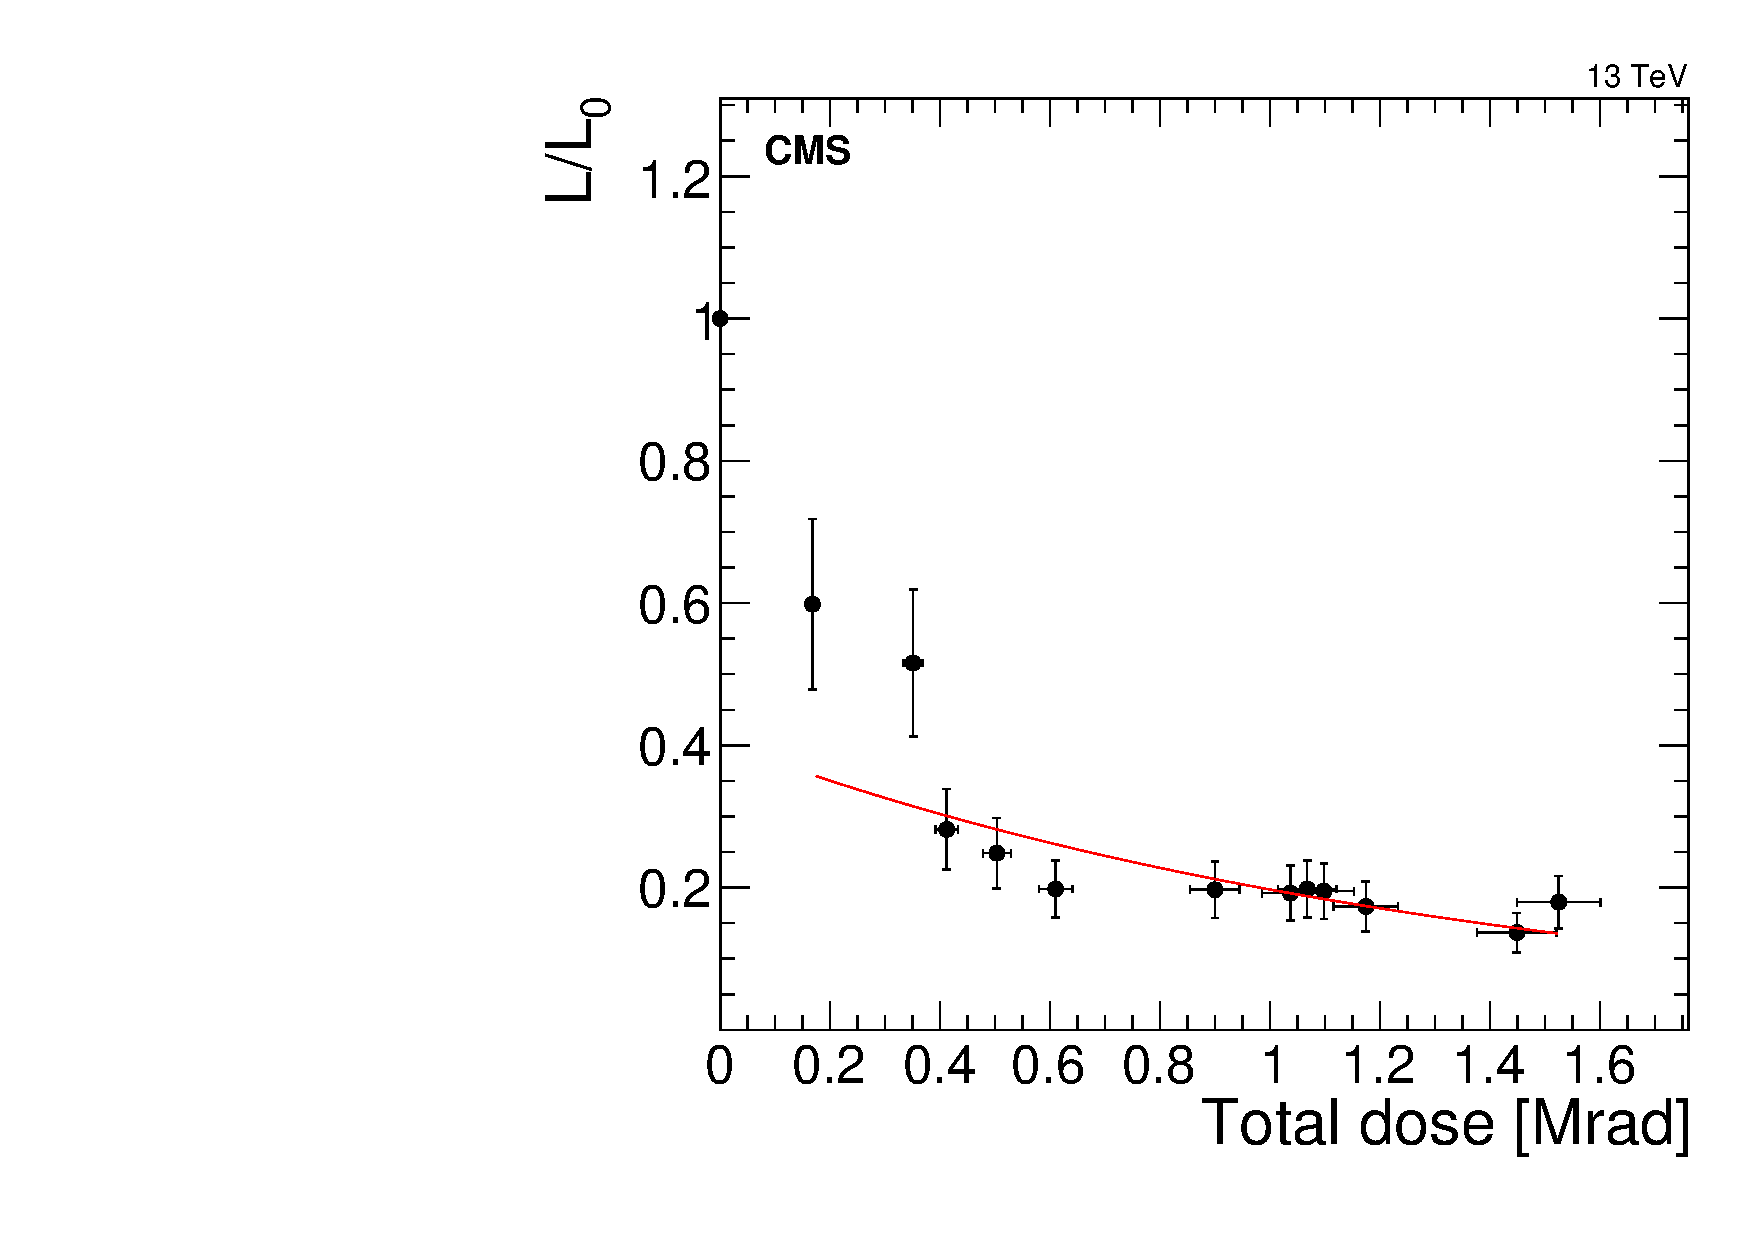
\includegraphics[width=0.45\textwidth]{figures/SCSN81-S-25p9cm-f7ch2-dose.pdf}
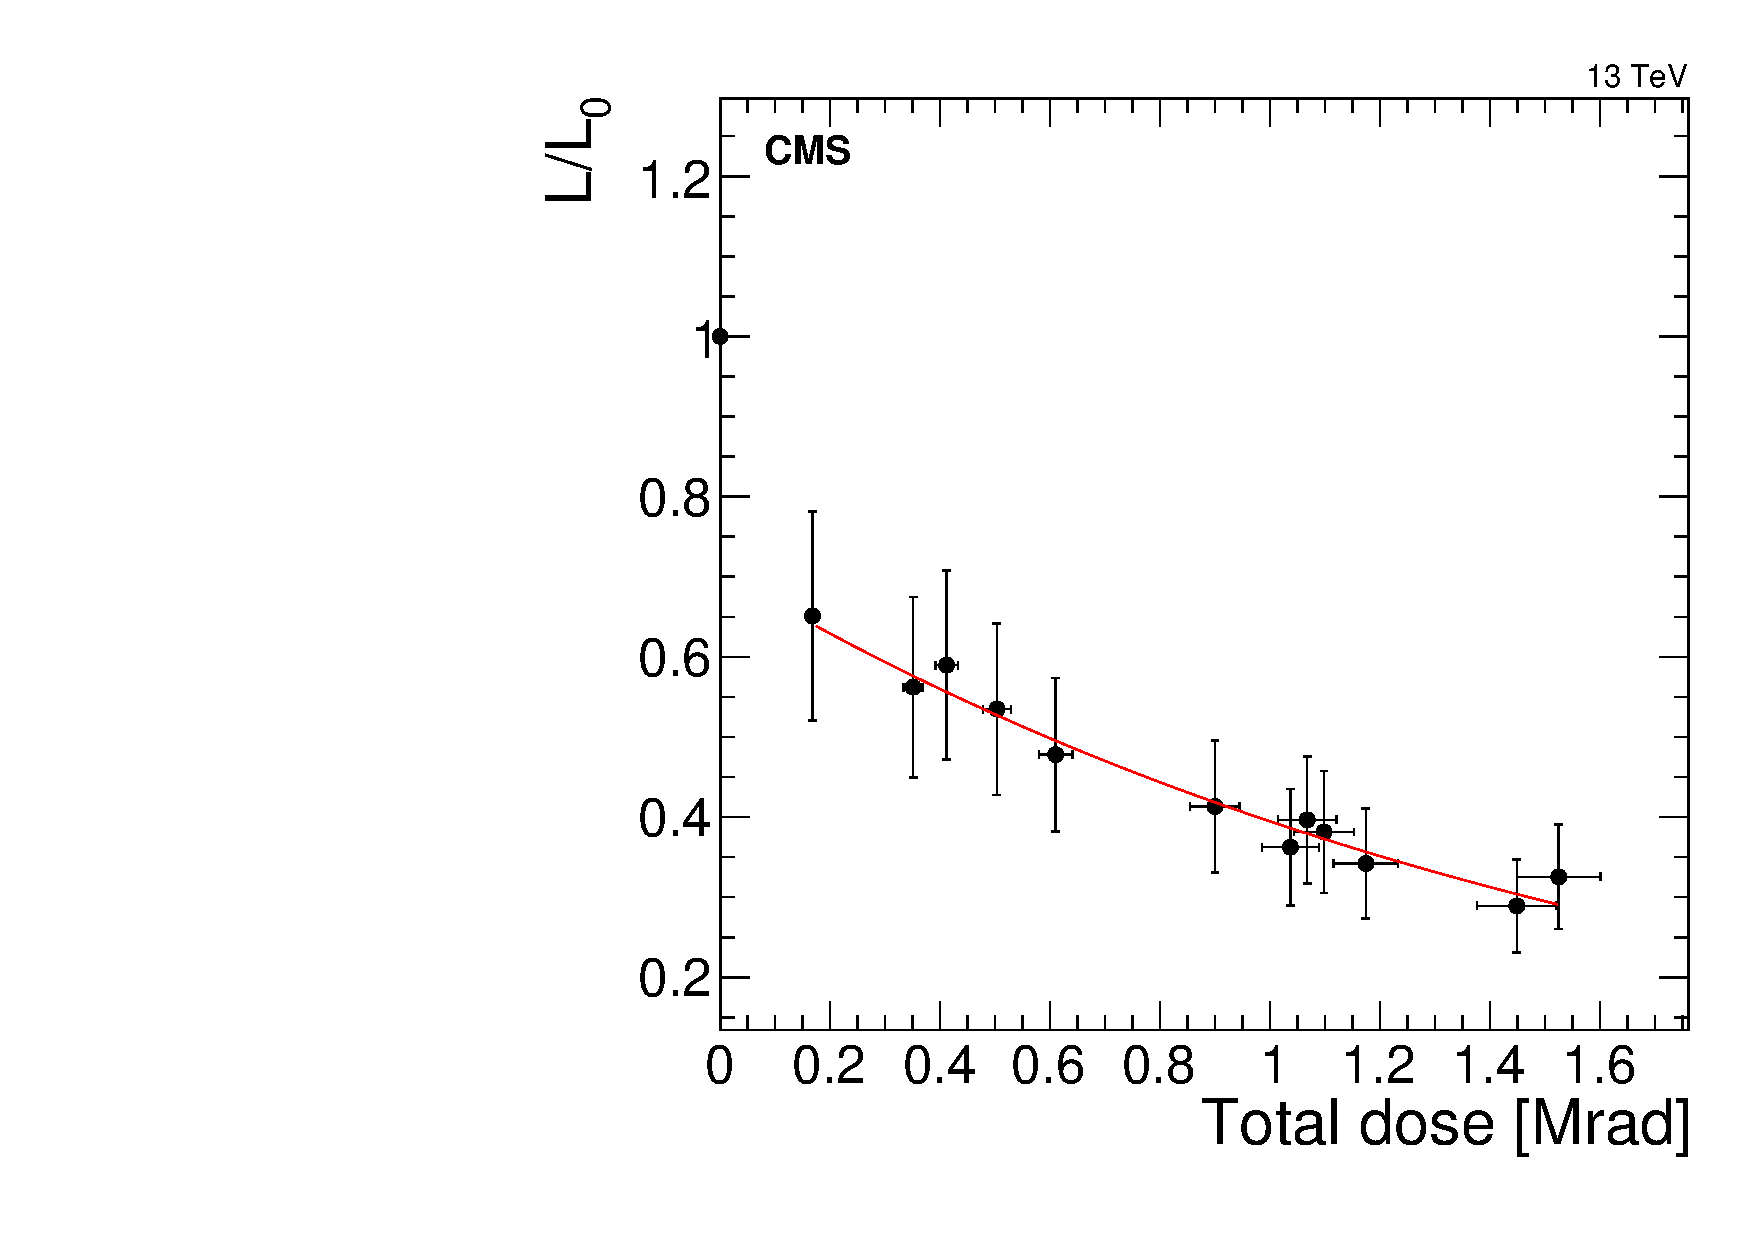
\includegraphics[width=0.45\textwidth]{figures/SCSN81-S-25p9cm-f8ch5-dose.pdf}
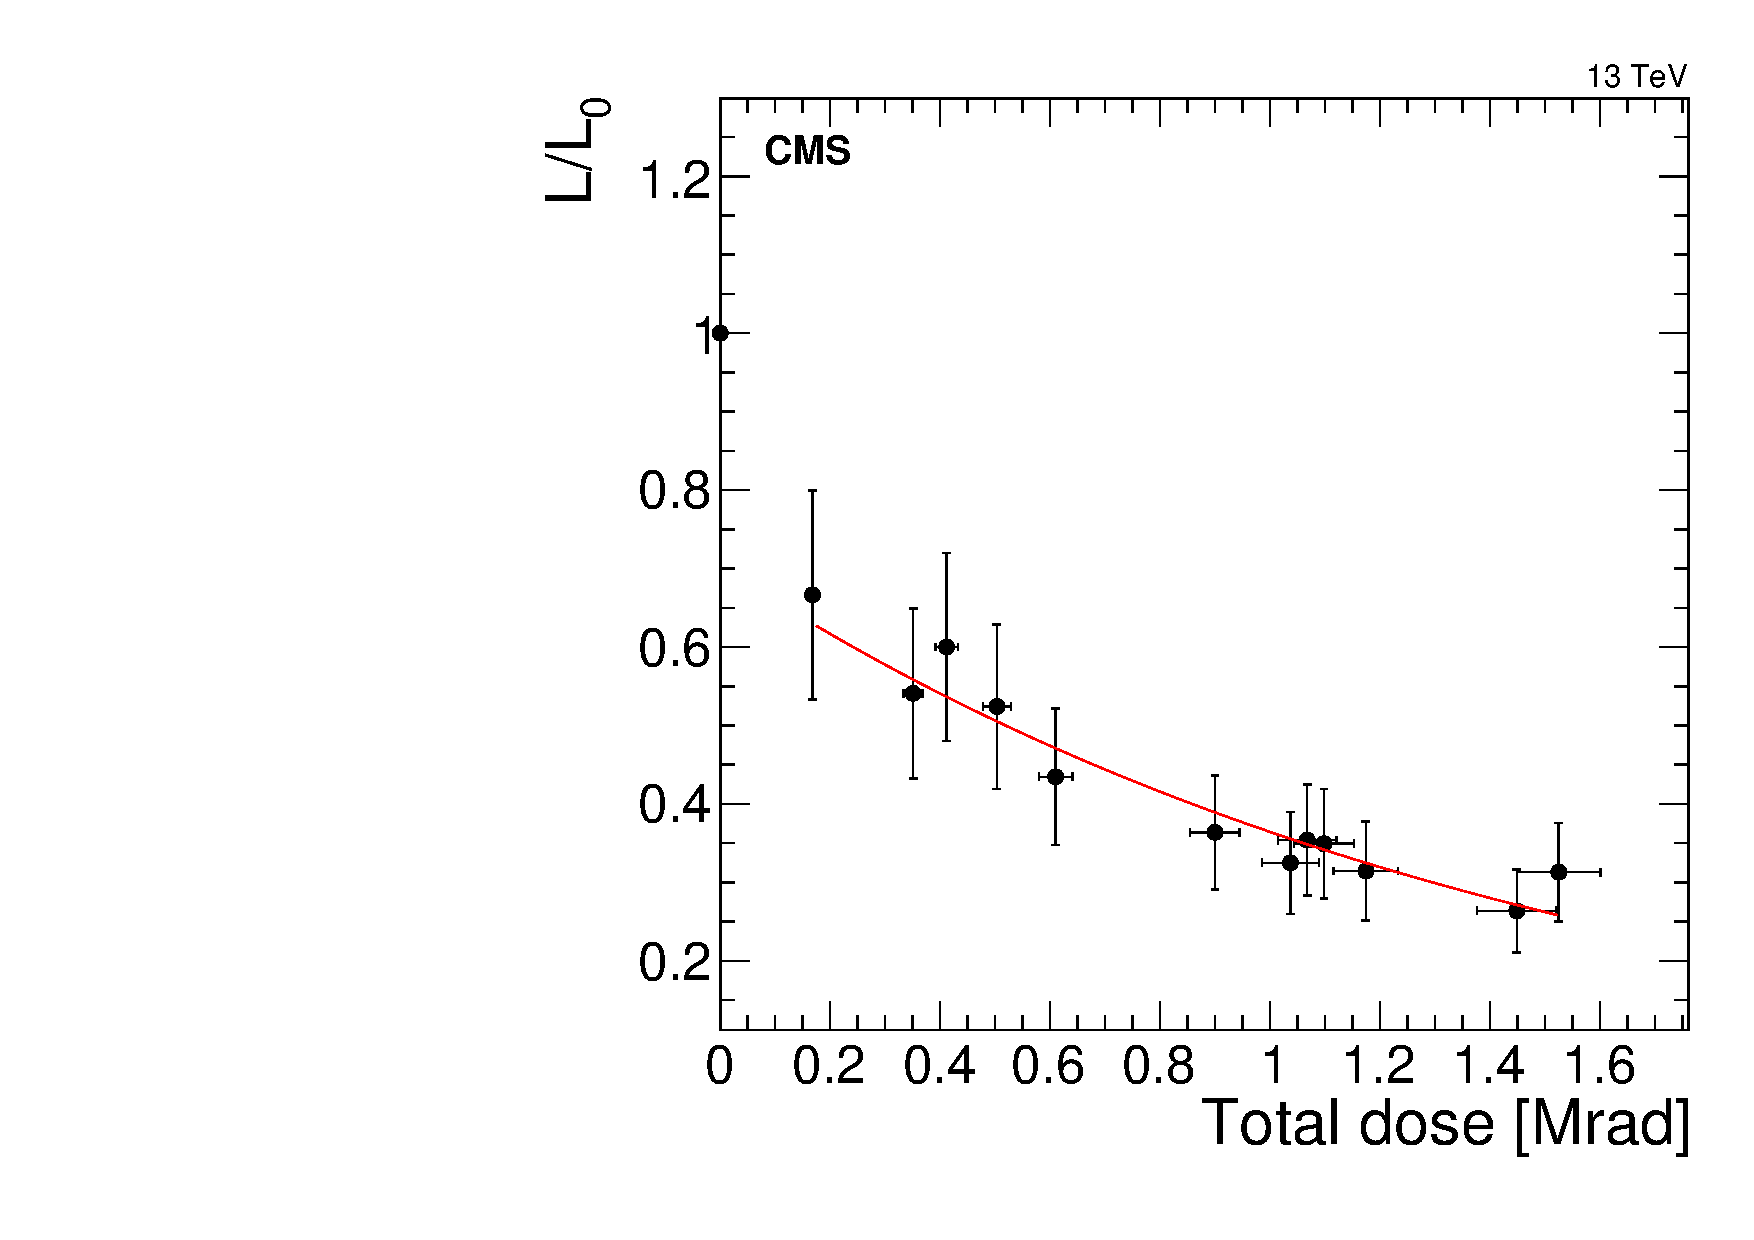
\includegraphics[width=0.45\textwidth]{figures/SCSN81-S-25p9cm-f14ch3-dose.pdf}
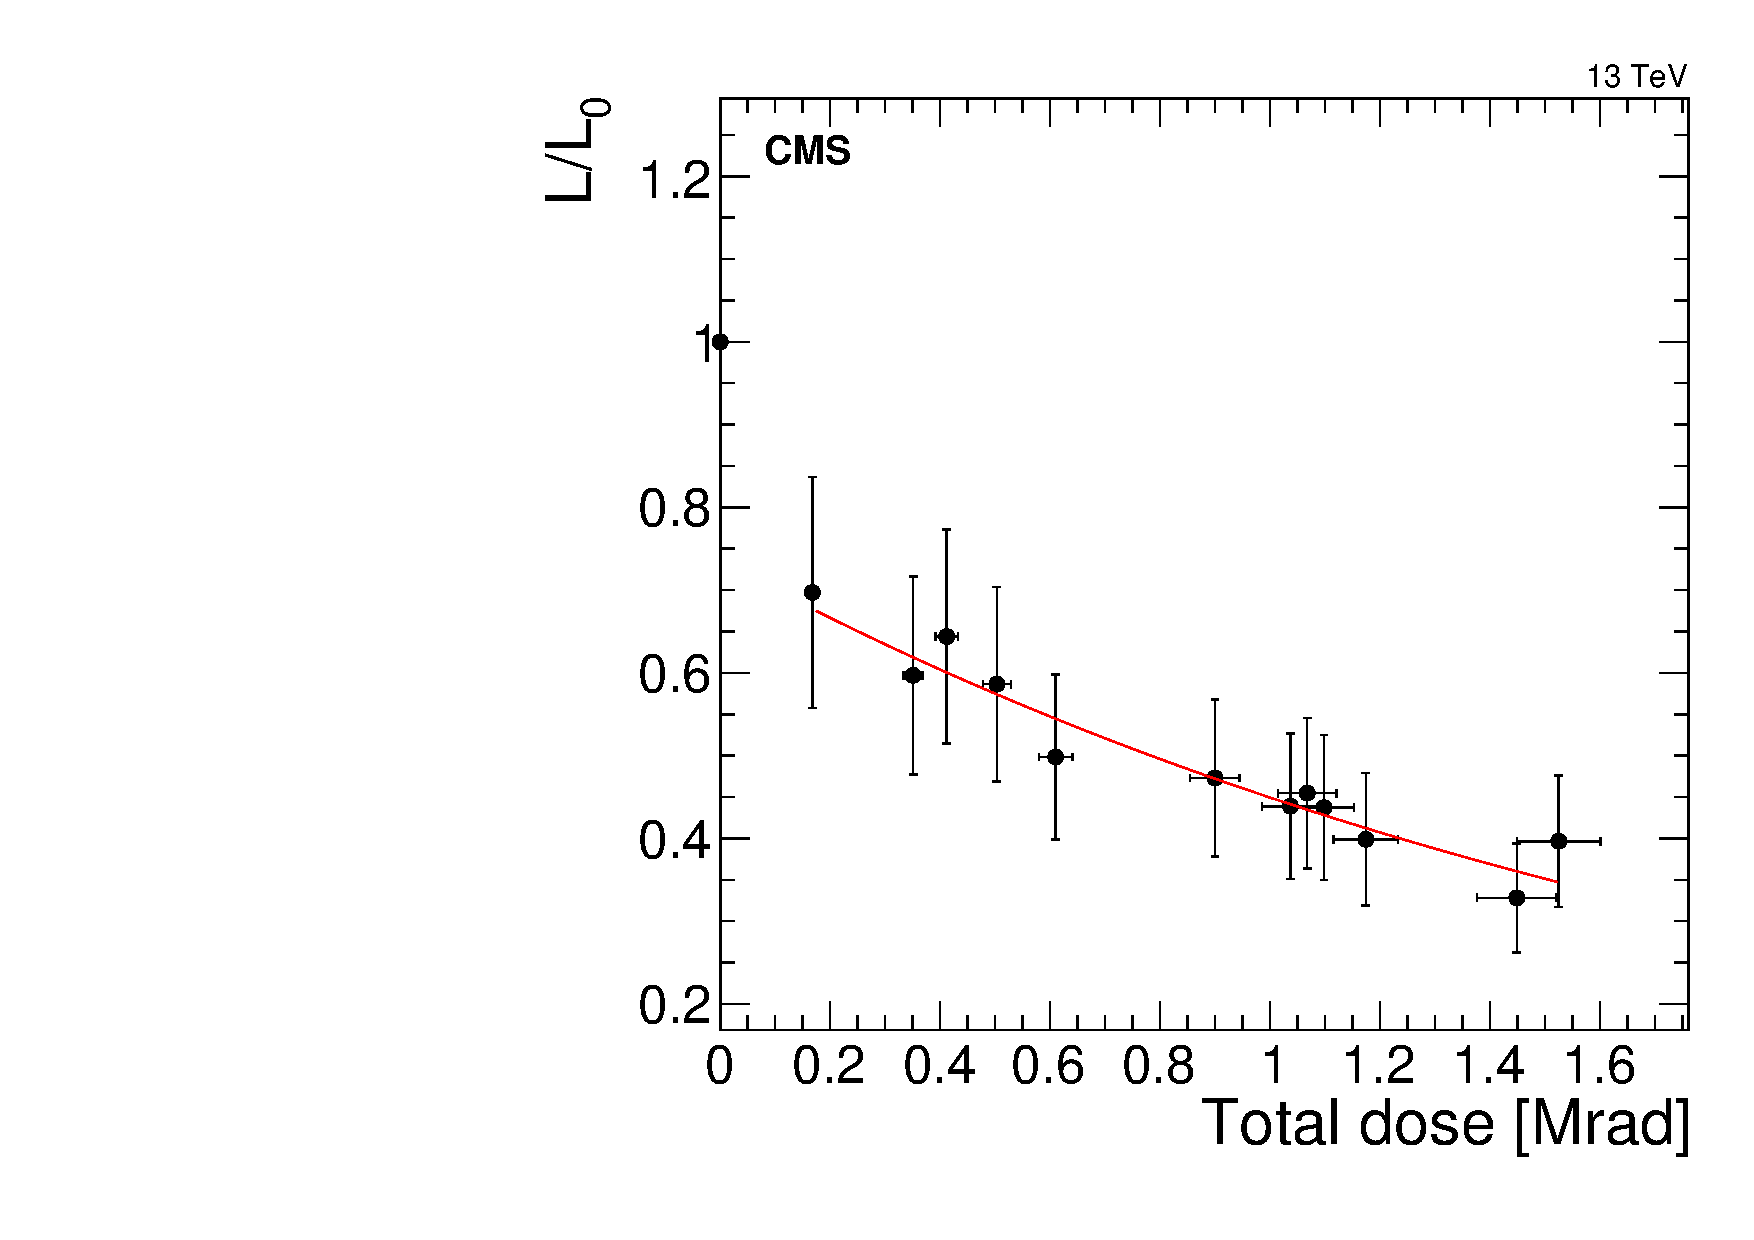
\includegraphics[width=0.45\textwidth]{figures/SCSN81-S-25p9cm-f16ch1-dose.pdf}
\caption{Relative yield versus integrated dose for SCSN81 sigma tiles at 25.9 cm from the CMS beam pipe, receiving 4.20 krad/hr. The exponential decay curve fitted to the steady-state region of light loss is shown in red.}
\label{fig:SCSN81-S-25p9cm-dose}
\end{figure} 

\begin{figure}[tbp!]
\centering
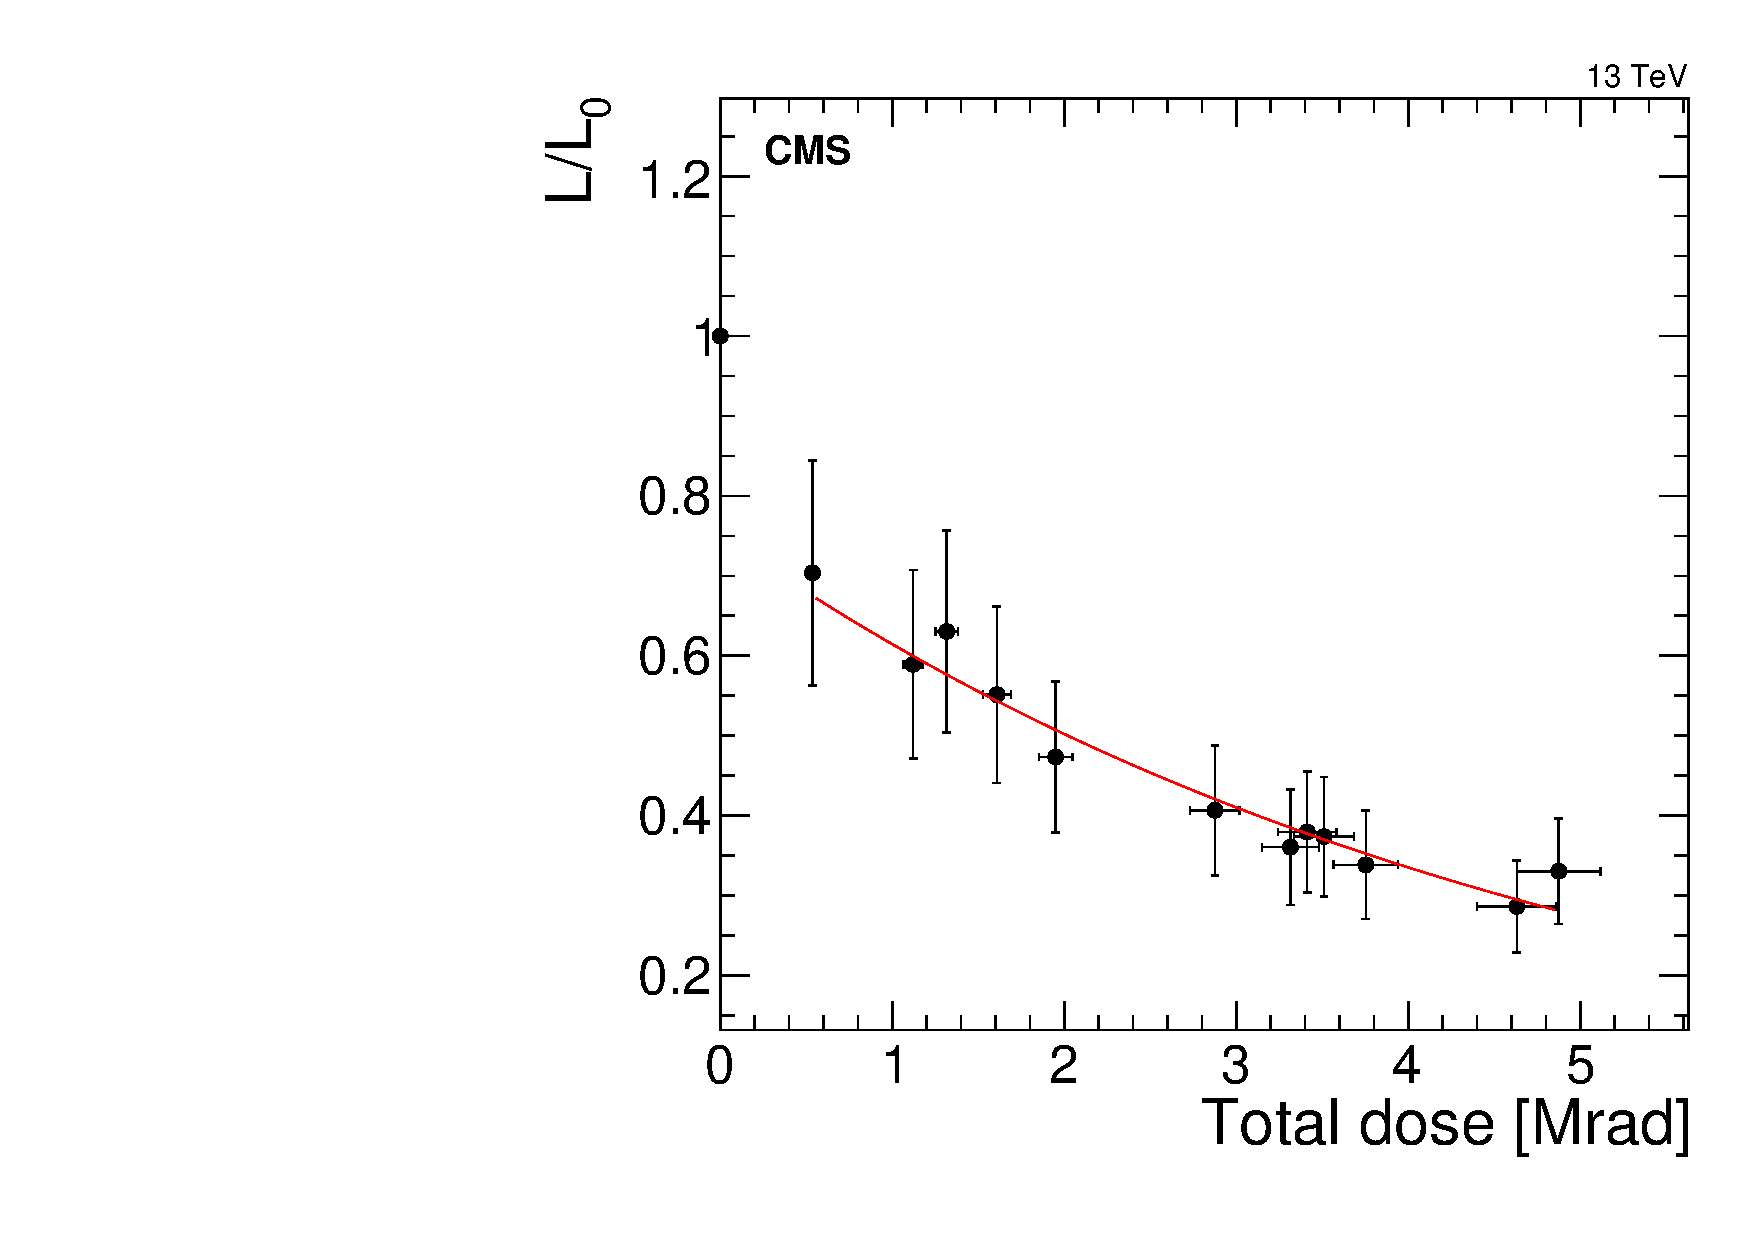
\includegraphics[width=0.45\textwidth]{figures/SCSN81-F-14p4cm-f4ch3-dose.pdf}
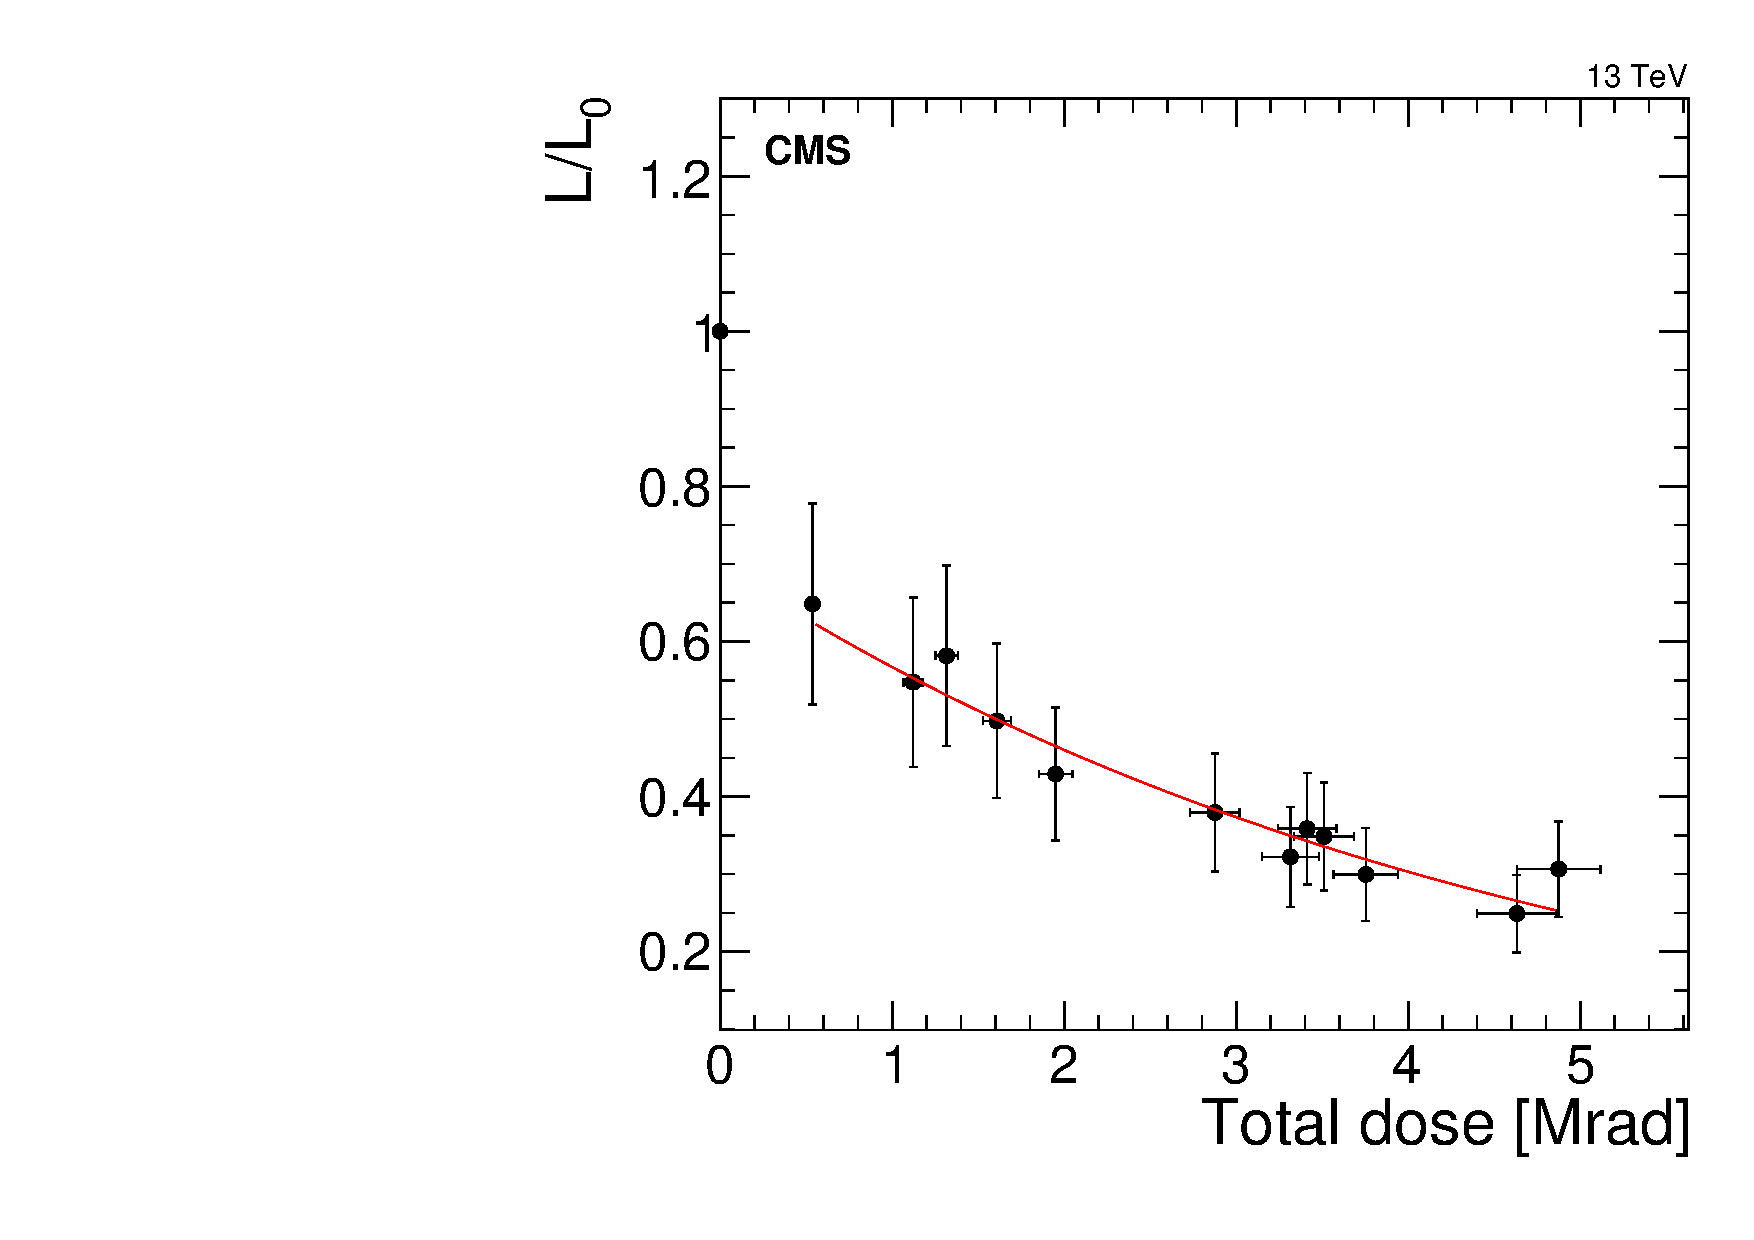
\includegraphics[width=0.45\textwidth]{figures/SCSN81-F-14p4cm-f7ch0-dose.pdf}
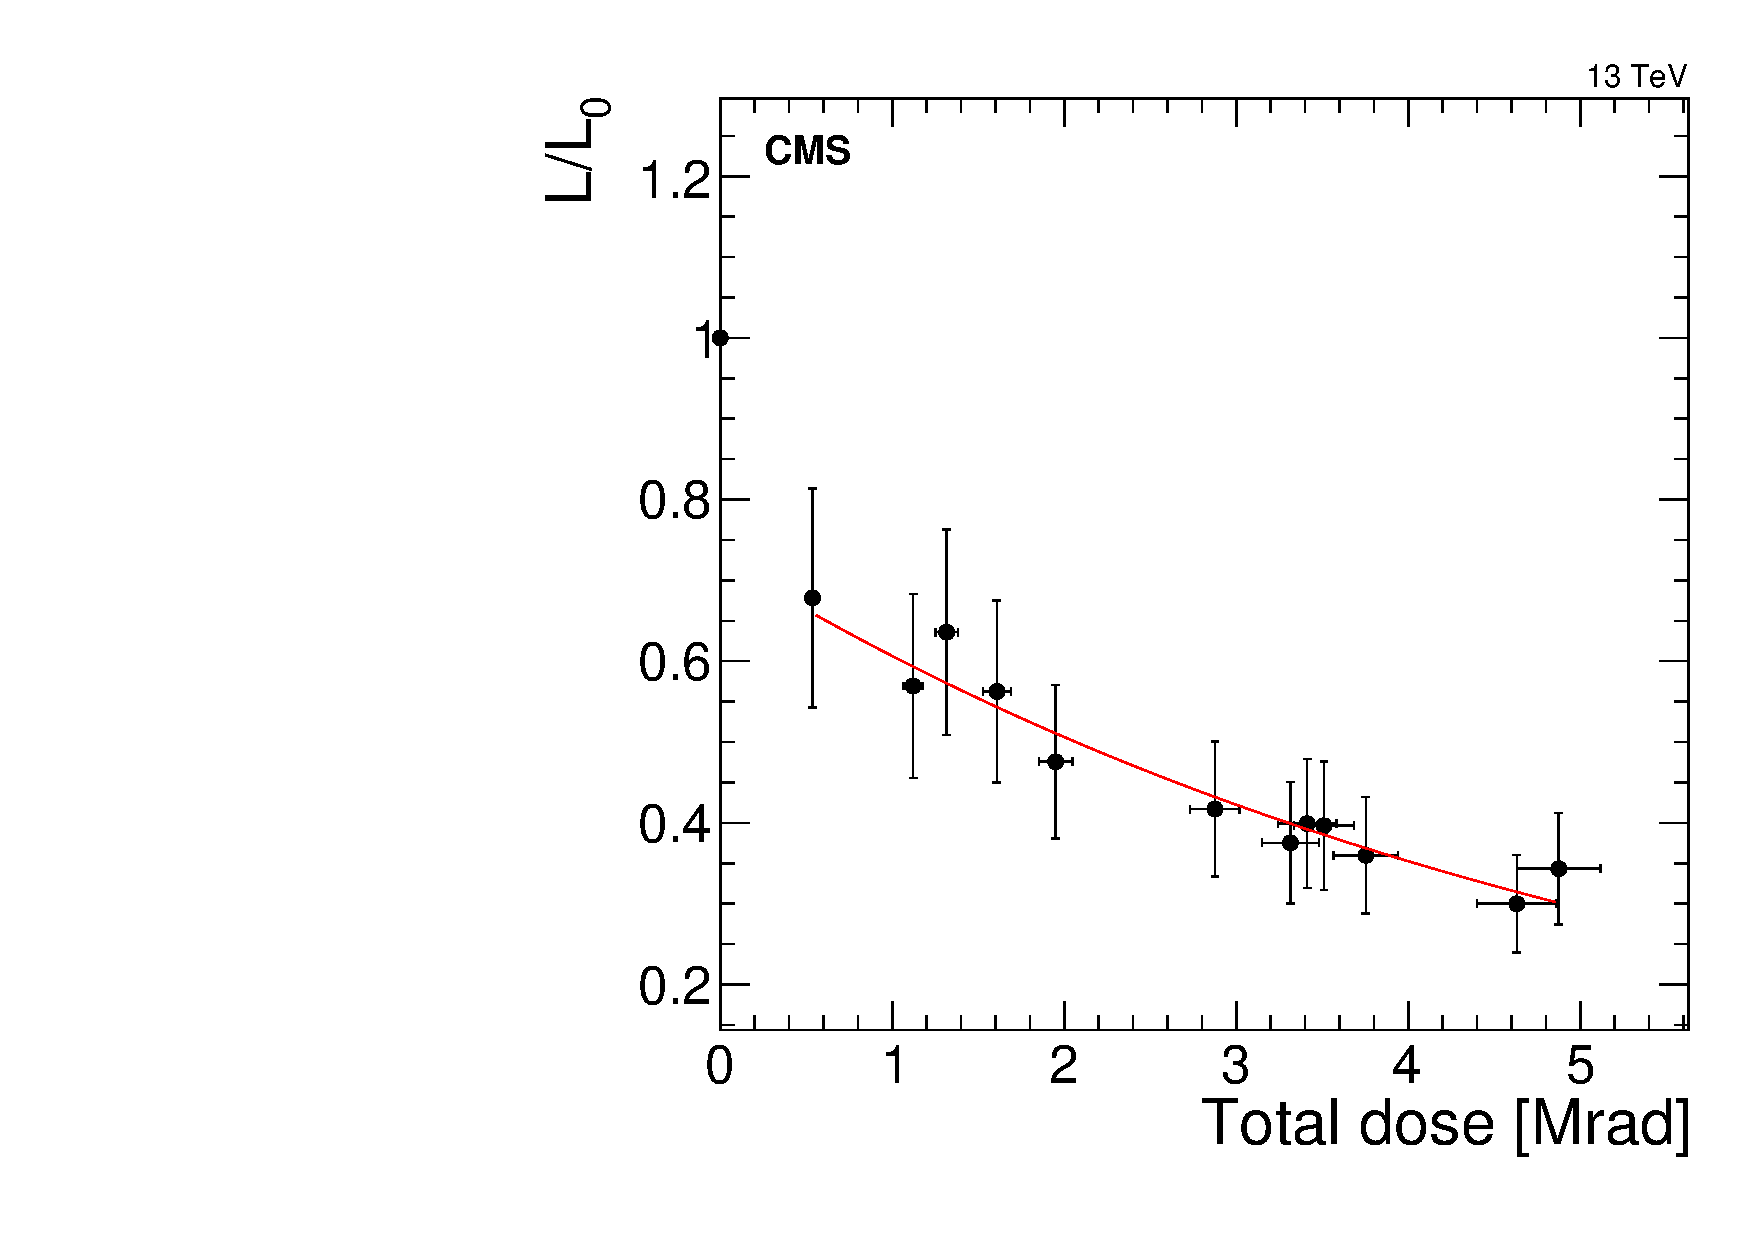
\includegraphics[width=0.45\textwidth]{figures/SCSN81-F-14p4cm-f18ch0-dose.pdf}
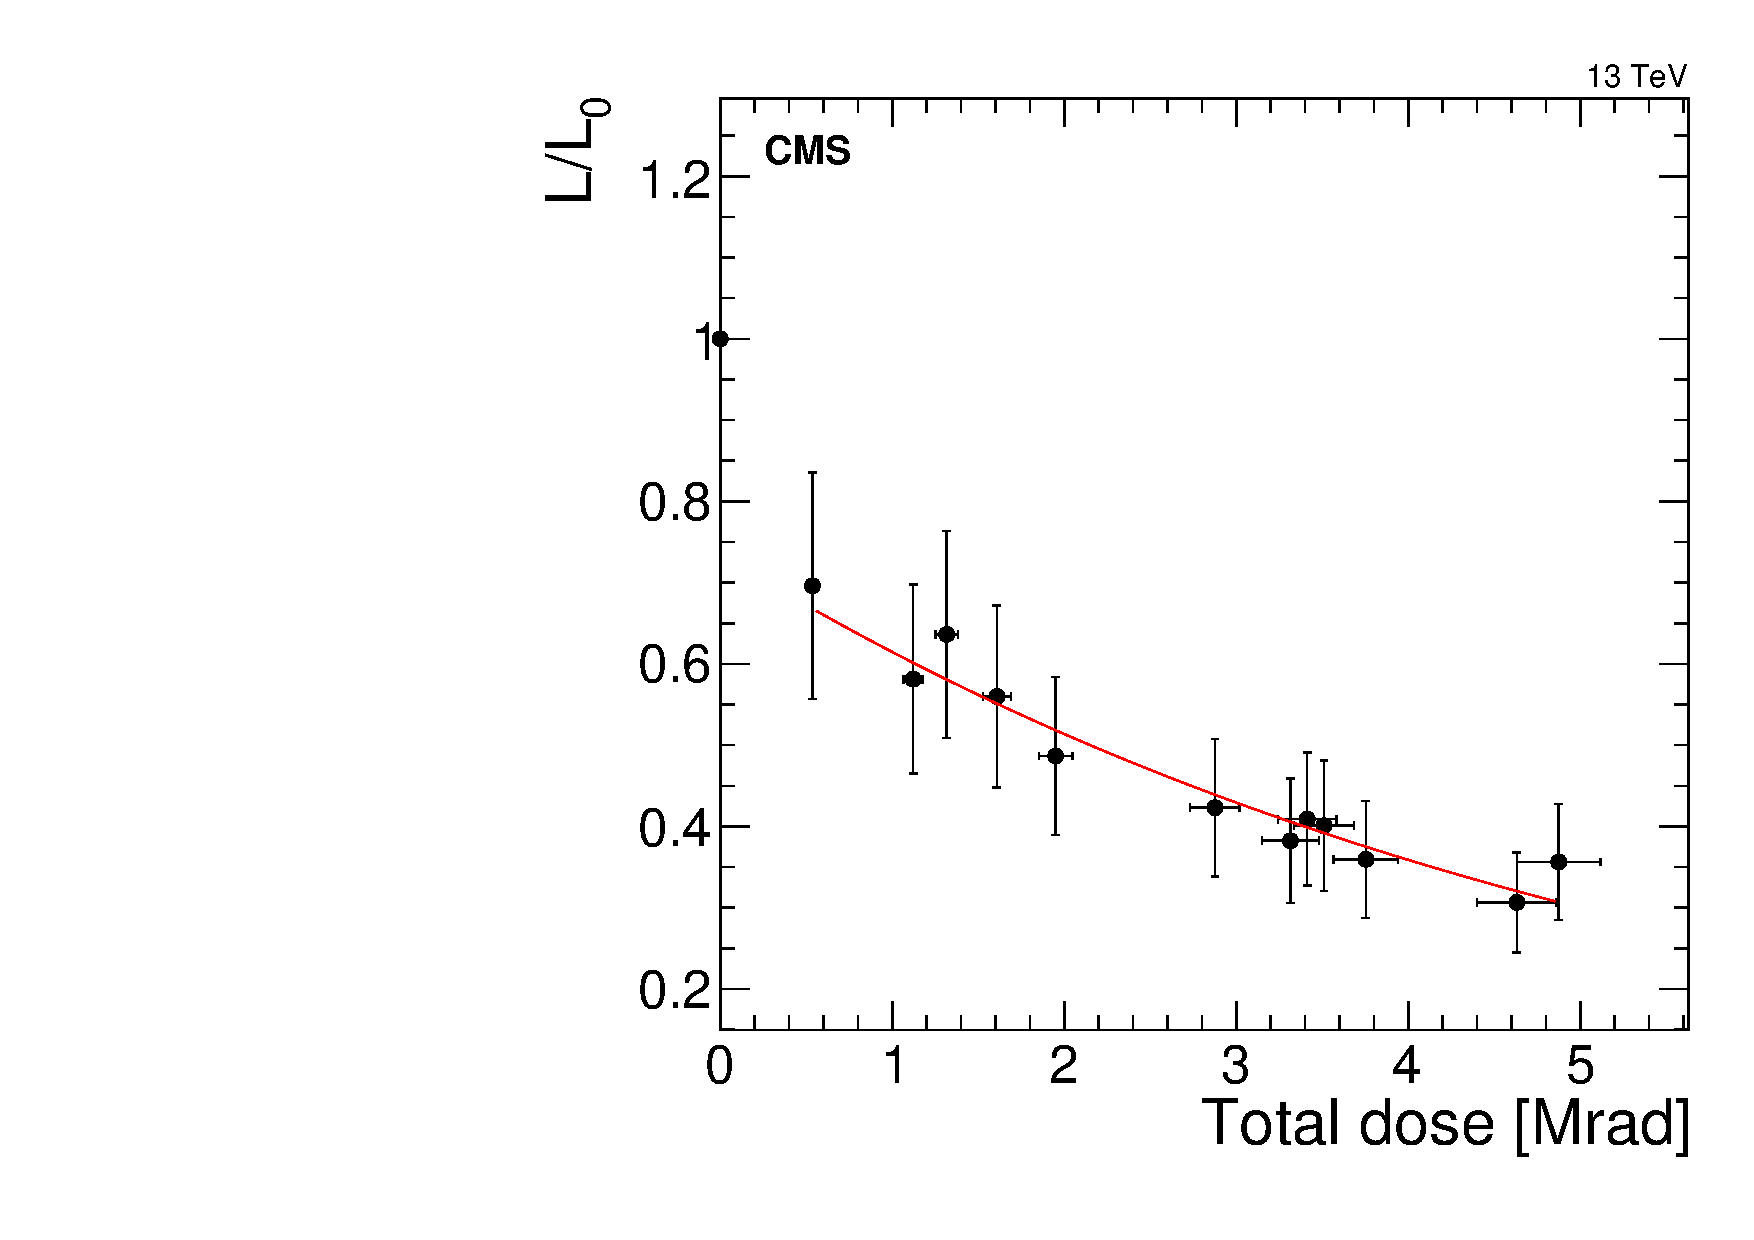
\includegraphics[width=0.45\textwidth]{figures/SCSN81-F-14p4cm-f18ch1-dose.pdf}
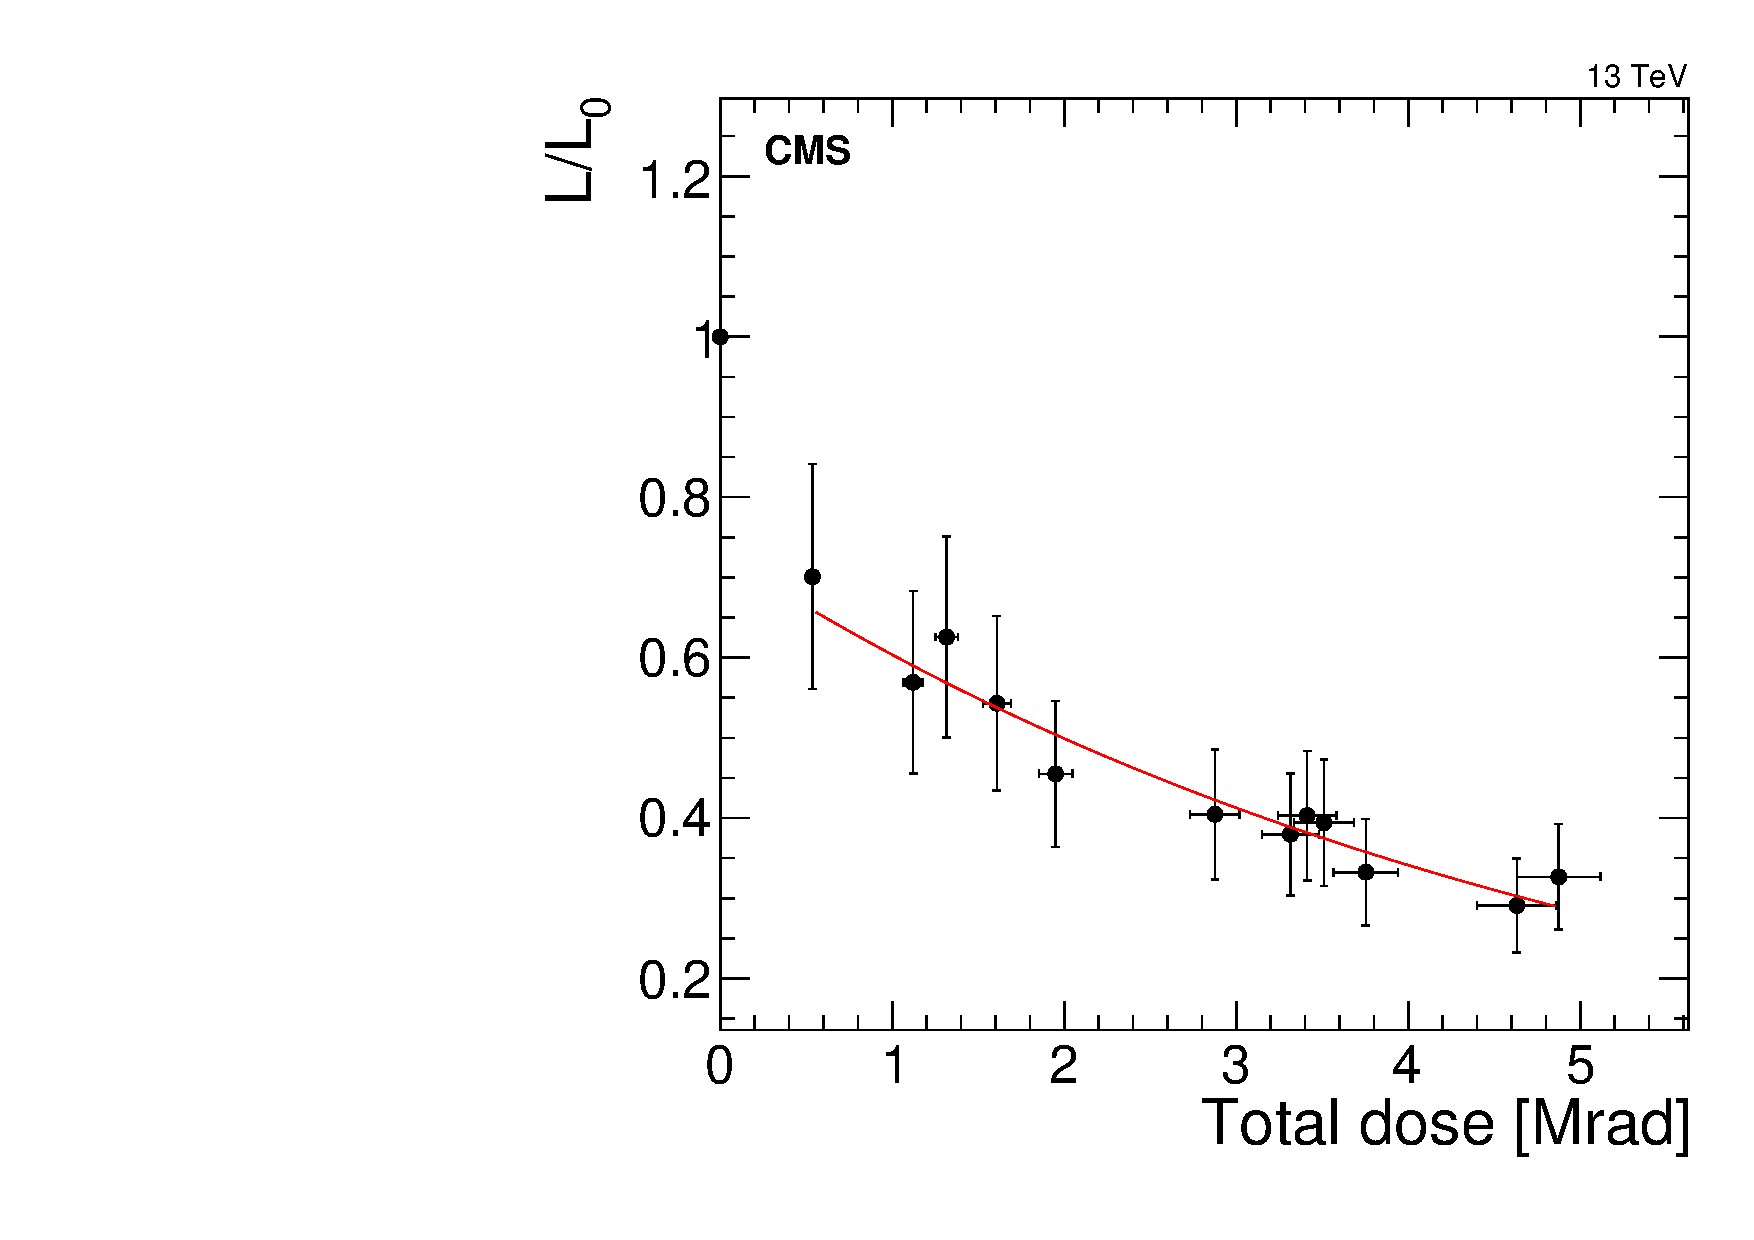
\includegraphics[width=0.45\textwidth]{figures/SCSN81-F-14p4cm-f18ch2-dose.pdf}
\caption{Relative yield versus integrated dose for SCSN81 finger tiles at 14.4 cm from the CMS beam pipe, receiving 13.44 krad/hr. The exponential decay curve fitted to the steady-state region of light loss is shown in red.}
\label{fig:SCSN81-F-14p4cm-dose}
\end{figure} 

\begin{figure}[tbp!]
\centering
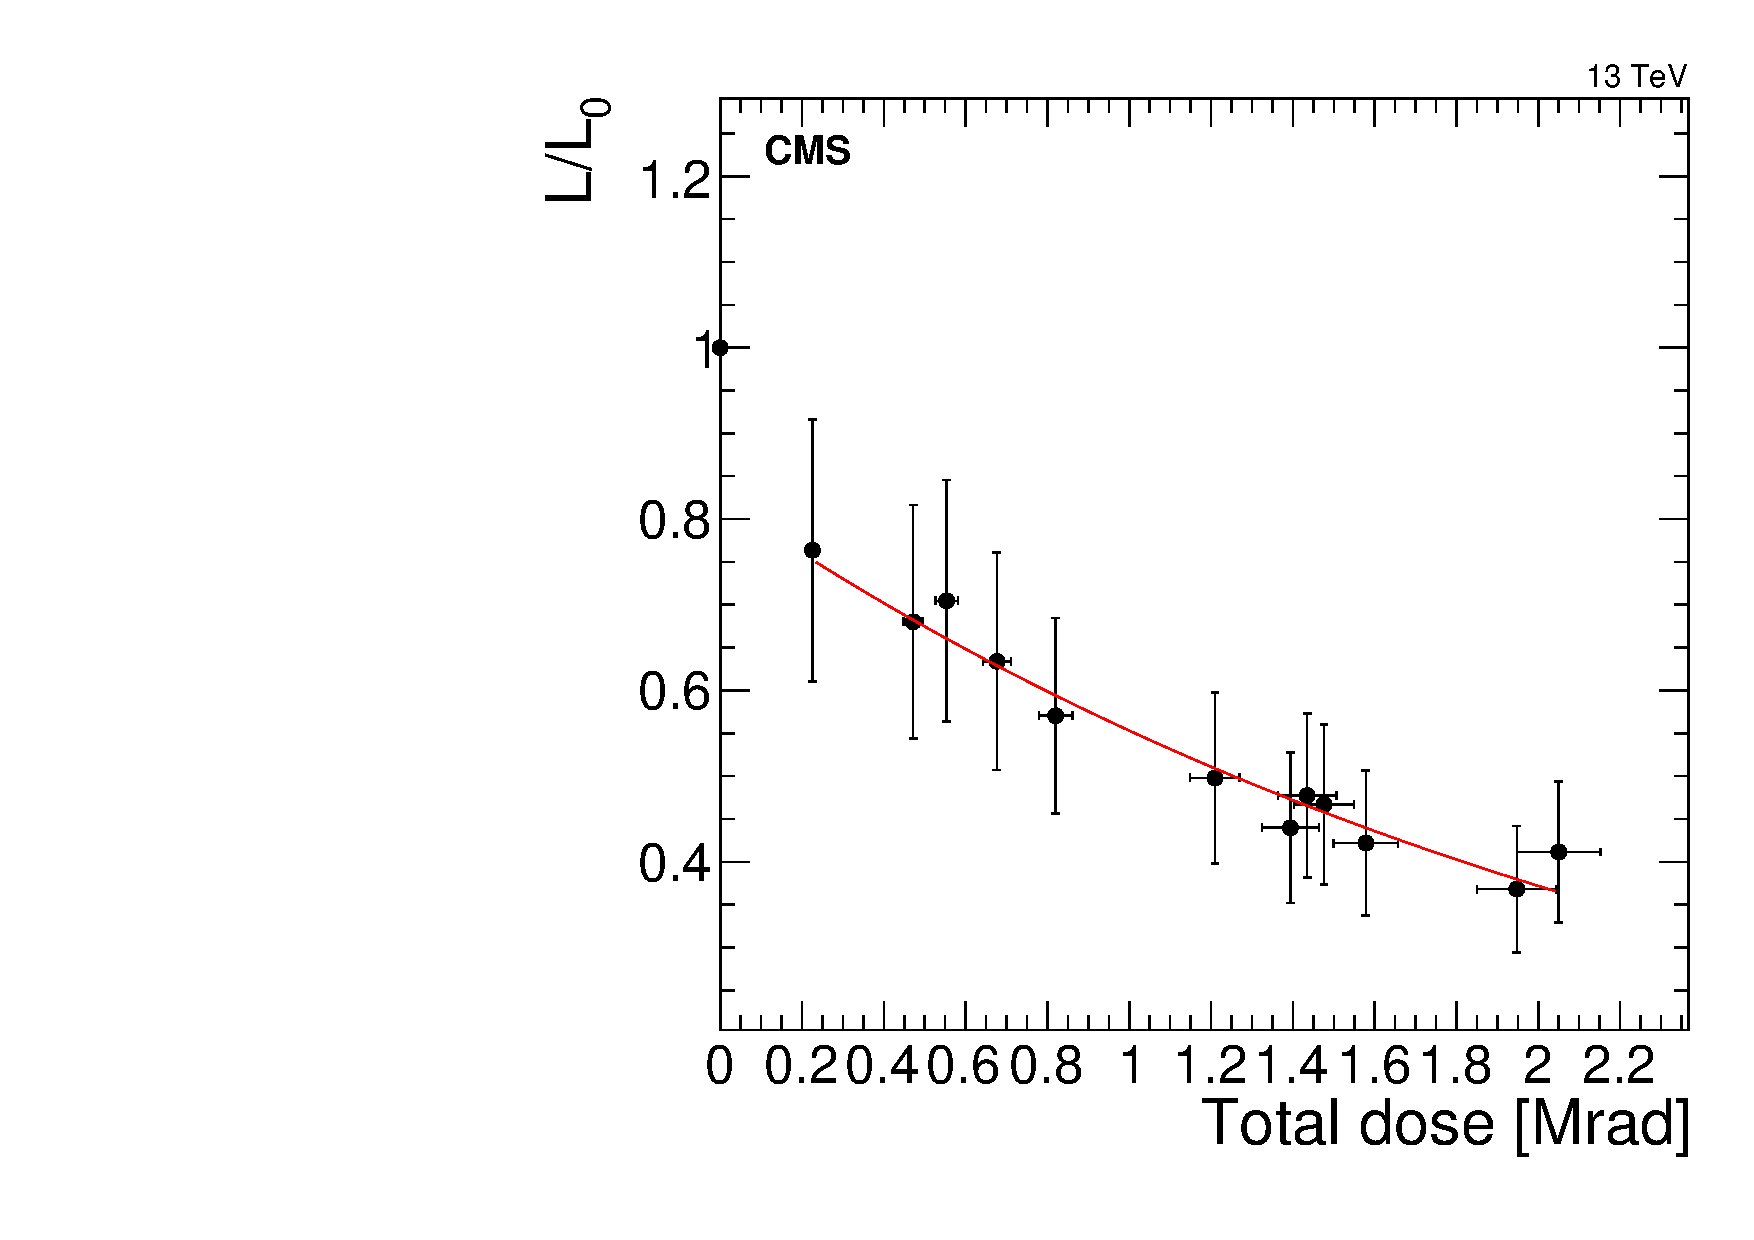
\includegraphics[width=0.45\textwidth]{figures/SCSN81-F-20p8cm-f2ch0-dose.pdf}
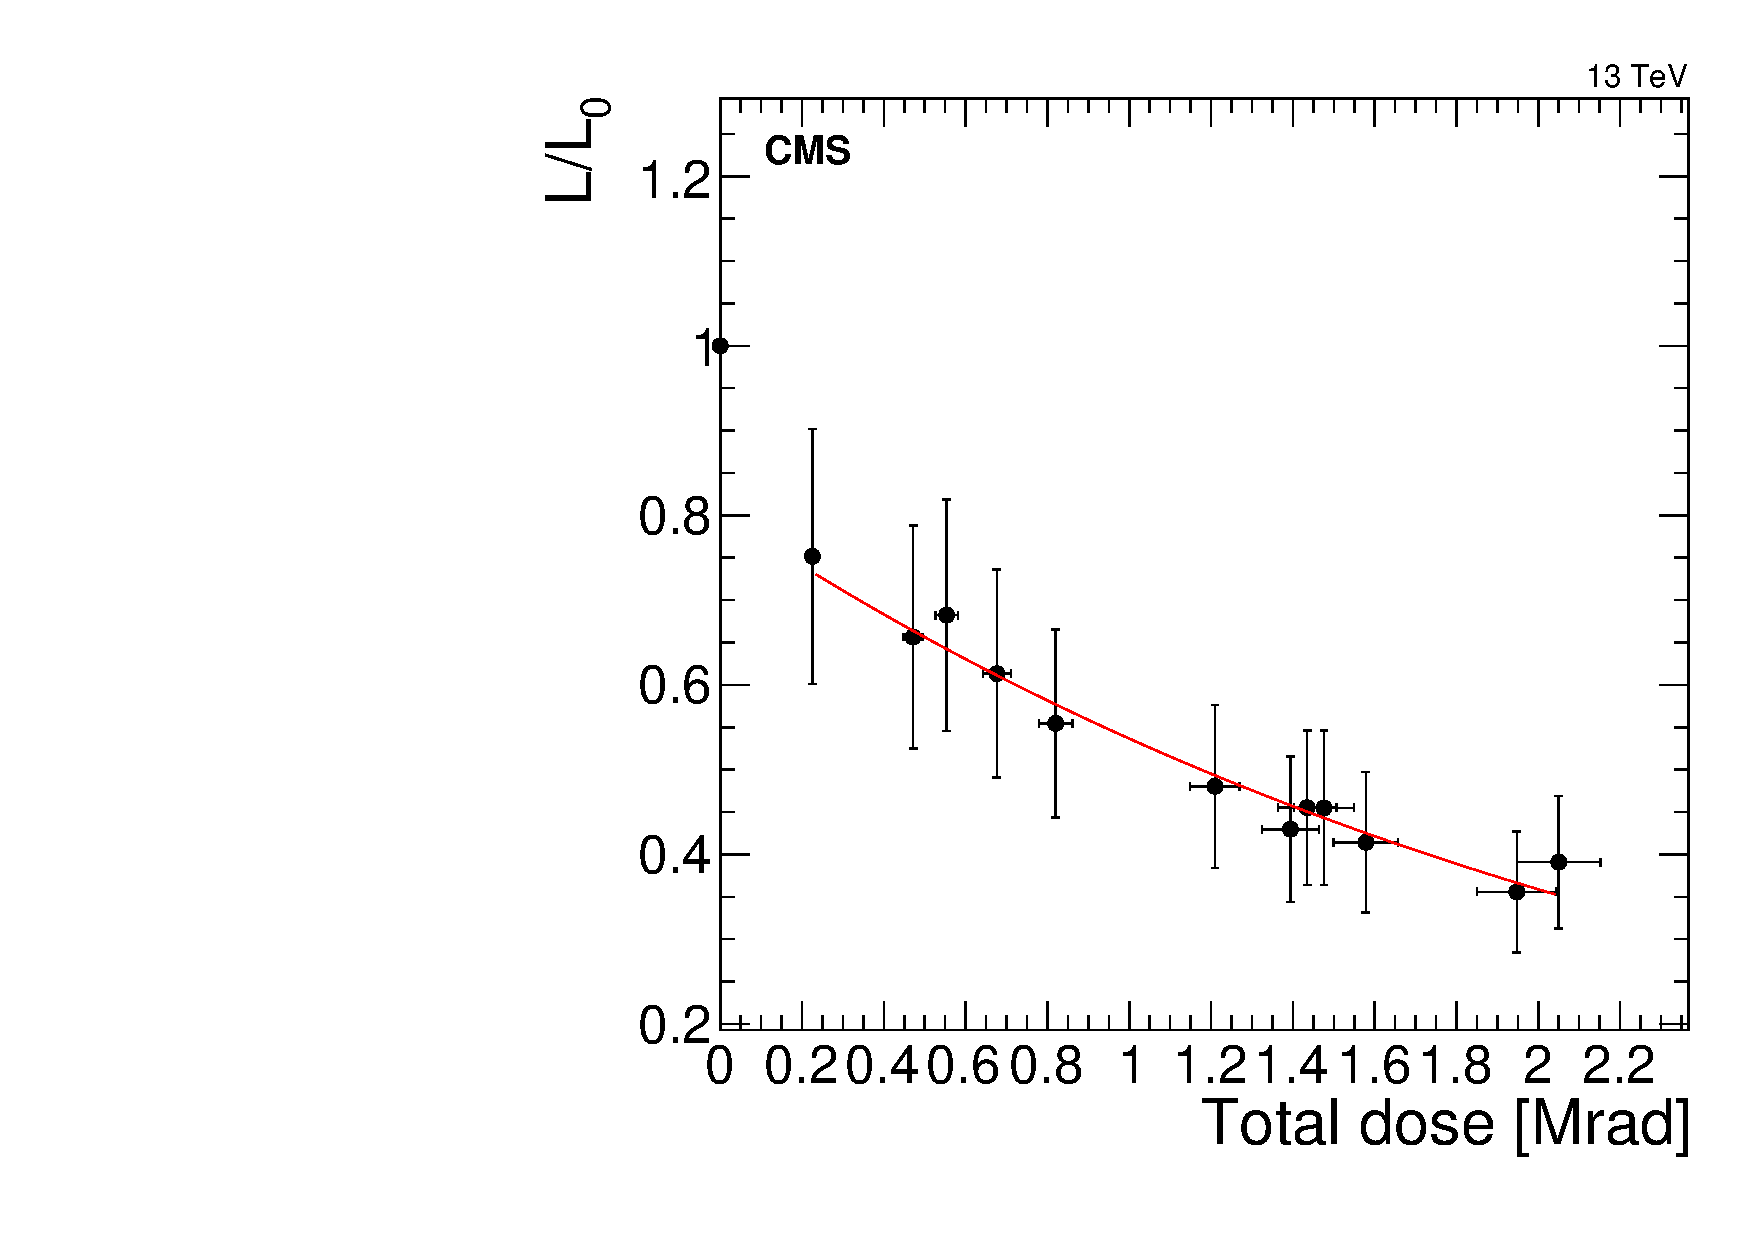
\includegraphics[width=0.45\textwidth]{figures/SCSN81-F-20p8cm-f4ch1-dose.pdf}
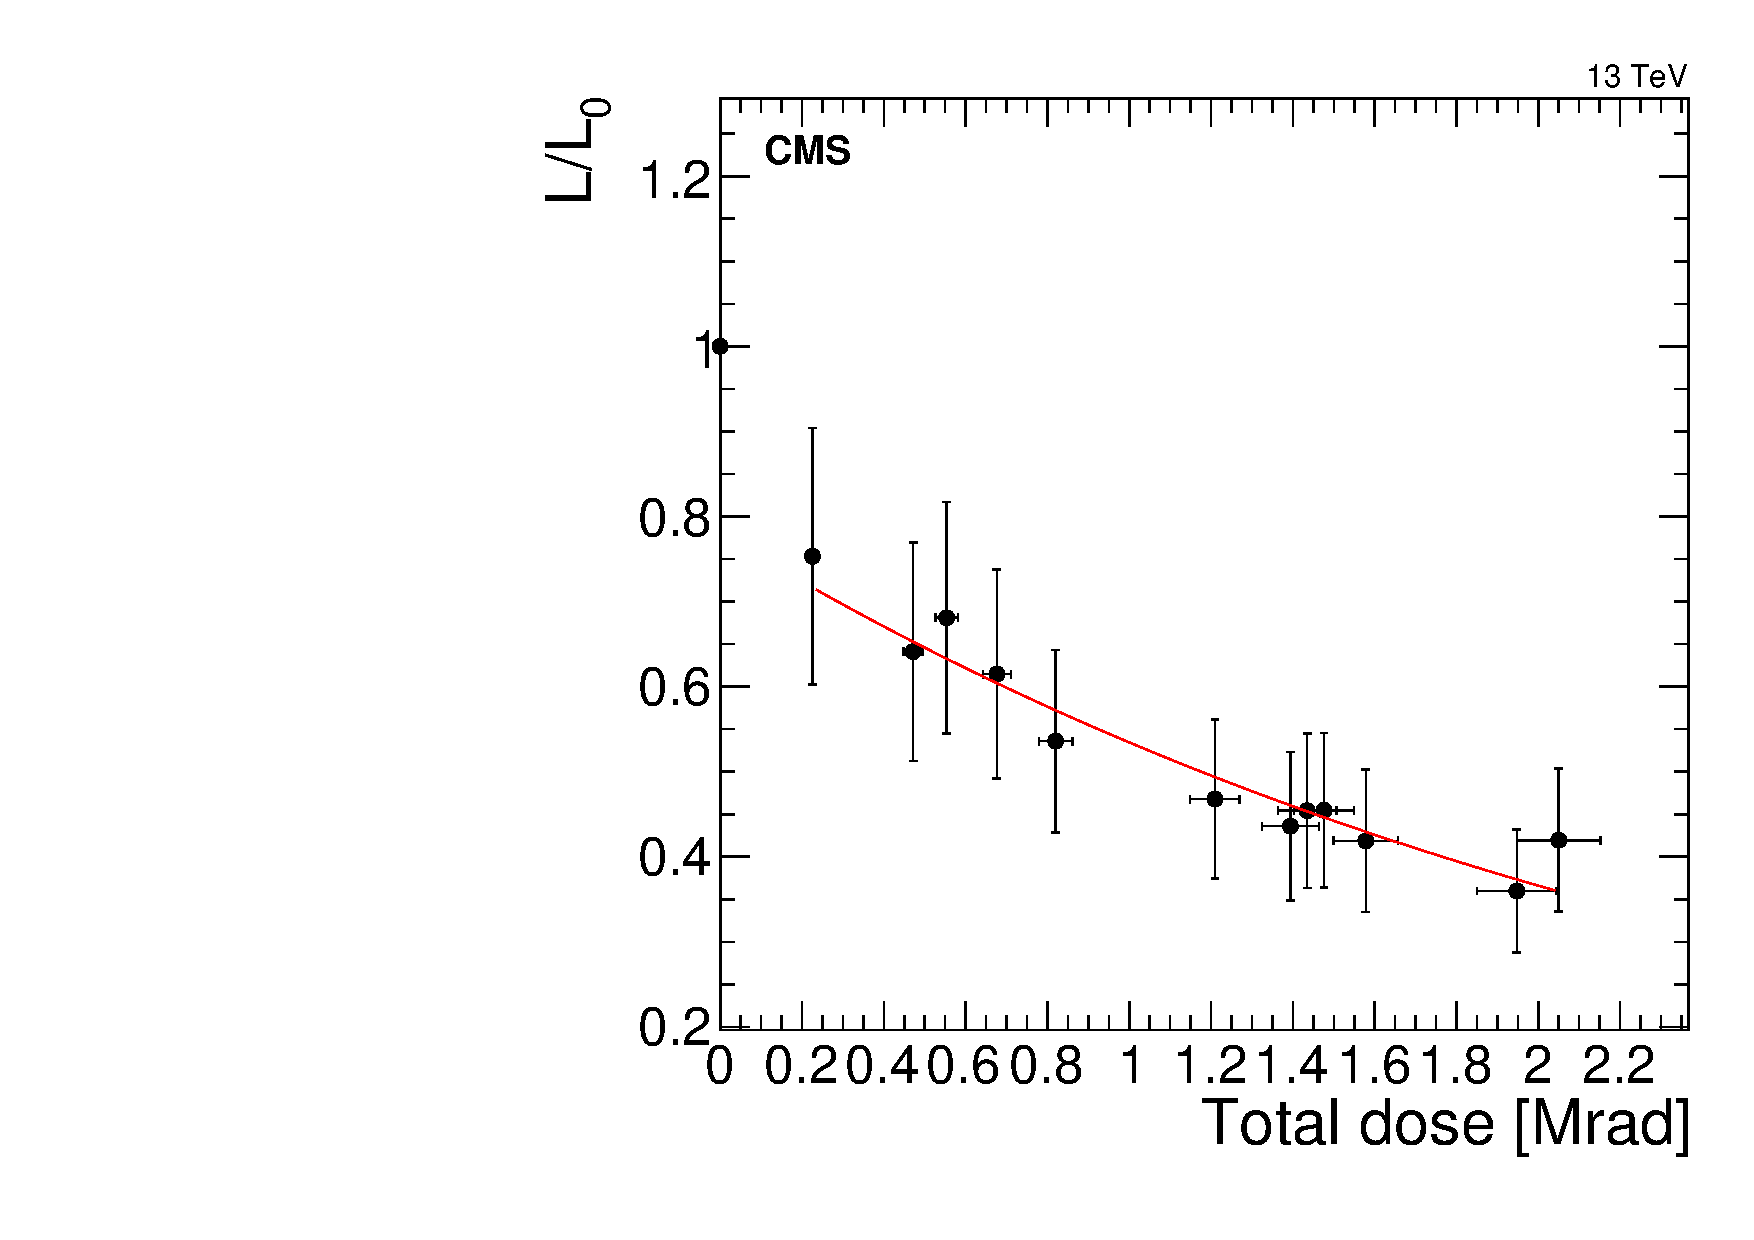
\includegraphics[width=0.45\textwidth]{figures/SCSN81-F-20p8cm-f15ch2-dose.pdf}
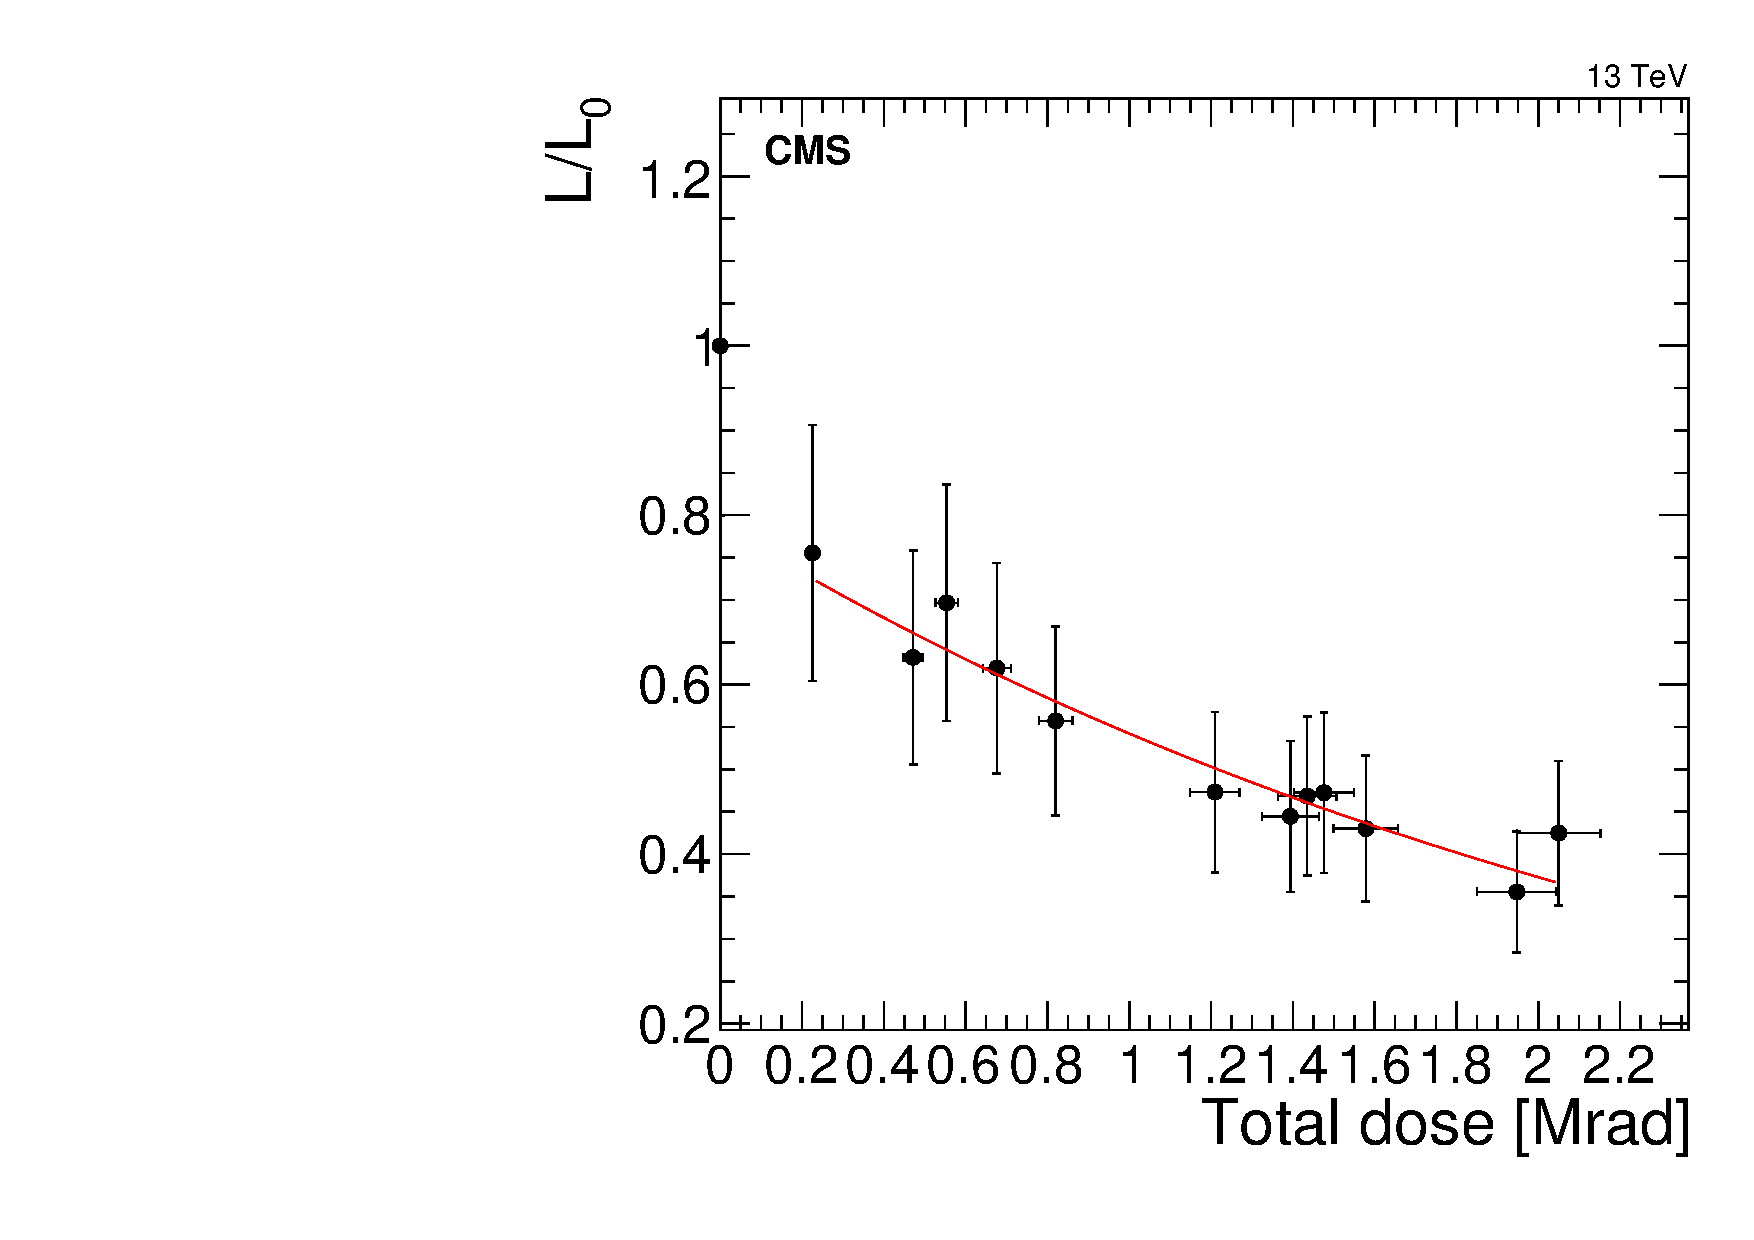
\includegraphics[width=0.45\textwidth]{figures/SCSN81-F-20p8cm-f15ch3-dose.pdf}
\includegraphics[width=0.45\textwidth]{figures/SCSN81-F-20p8cm-f20ch2-dose.pdf}
\includegraphics[width=0.45\textwidth]{figures/SCSN81-F-20p8cm-f20ch3-dose.pdf}
\caption{Relative yield versus integrated dose for SCSN81 finger tiles at 20.8 cm from the CMS beam pipe, receiving 5.65 krad/hr. The exponential decay curve fitted to the steady-state region of light loss is shown in red.}
\label{fig:SCSN81-F-20p8cm-dose}
\end{figure} 

\begin{figure}[tbp!]
\centering
\includegraphics[width=0.32\textwidth]{figures/SCSN81-F-27p2cm-f2ch5-dose.pdf}
\includegraphics[width=0.32\textwidth]{figures/SCSN81-F-27p2cm-f3ch5-dose.pdf}
\includegraphics[width=0.32\textwidth]{figures/SCSN81-F-27p2cm-f4ch0-dose.pdf}
\includegraphics[width=0.32\textwidth]{figures/SCSN81-F-27p2cm-f6ch1-dose.pdf}
\includegraphics[width=0.32\textwidth]{figures/SCSN81-F-27p2cm-f8ch4-dose.pdf}
\includegraphics[width=0.32\textwidth]{figures/SCSN81-F-27p2cm-f14ch2-dose.pdf}
\includegraphics[width=0.32\textwidth]{figures/SCSN81-F-27p2cm-f14ch5-dose.pdf}
\includegraphics[width=0.32\textwidth]{figures/SCSN81-F-27p2cm-f16ch0-dose.pdf}
\caption{Relative yield versus integrated dose for SCSN81 finger tiles at 27.2 cm from the CMS beam pipe, receiving 3.93 krad/hr. The exponential decay curve fitted to the steady-state region of light loss is shown in red.}
\label{fig:SCSN81-F-27p2cm-dose}
\end{figure} 

\begin{figure}[tbp!]
\centering
\includegraphics[width=0.45\textwidth]{figures/EJ200-S-11p8cm-f18ch5-dose.pdf}
\includegraphics[width=0.45\textwidth]{figures/EJ200-S-25p9cm-f15ch5-dose.pdf}
\caption{Relative yield versus integrated dose for EJ200 sigma tiles. (\cmsLeft) Tile at 11.8 cm from the CMS beam pipe, receiving 16.61 krad/hr. (\cmsRight) Tile at 25.9 cm from the beam pipe, receiving 4.20 krad/hr. The exponential decay curve fitted to the steady-state region of light loss is shown in red.}
\label{fig:EJ200-S-dose}
\end{figure} 

\begin{figure}[tbp!]
\centering
\includegraphics[width=0.45\textwidth]{figures/EJ260-S-11p8cm-f8ch2-dose.pdf}
\includegraphics[width=0.45\textwidth]{figures/EJ260-S-18p2cm-f3ch1-dose.pdf}
\caption{Relative yield versus integrated dose for EJ260 sigma tiles. (\cmsLeft) Tile at 11.8 cm from the CMS beam pipe, receiving 16.61 krad/hr. (\cmsRight) Tile at 18.2 cm from the beam pipe, receiving 6.89 krad/hr. The exponential decay curve fitted to the steady-state region of light loss is shown in red.}
\label{fig:EJ260-S-dose}
\end{figure} 

\begin{figure}[tbp!]
\centering
\includegraphics[width=0.45\textwidth]{figures/EJ260-F-14p4cm-f6ch0-dose.pdf}
\includegraphics[width=0.45\textwidth]{figures/EJ260-F-14p4cm-f8ch1-dose.pdf}
\includegraphics[width=0.45\textwidth]{figures/EJ260-F-20p8cm-f3ch4-dose.pdf}
\includegraphics[width=0.45\textwidth]{figures/EJ260-F-20p8cm-f7ch1-dose.pdf}
\includegraphics[width=0.45\textwidth]{figures/EJ260-F-27p2cm-f8ch3-dose.pdf}
\caption{Relative yield versus integrated dose for EJ260 finger tiles. Top left and right: tiles at 14.4 cm from the CMS beam pipe, receiving 13.44 krad/hr. Middle left and right: tiles at 20.8 cm from the beam pipe, receiving 5.65 krad/hr. Bottom: tile at 27.2 cm from the beam pipe, receiving 3.93 krad/hr. The exponential decay curve fitted to the steady-state region of light loss is shown in red.}
\label{fig:EJ260-F-dose}
\end{figure} 


\subsubsection{Light yield versus time\label{sec:ana-res-lyvstime}}

The relative light yields for the various tiles as a function of the number of days after the start of irradiation are shown here in Figures~\ref{fig:SCSN81-S-11p8cm-time} to~\ref{fig:EJ260-F-time}. Day 0 refers to the day when the tiles were installed on the CASTOR table, before irradiation. Irradiation began on day 2 and ended on day 42, after which some recovery in the relative light yield can be observed in most of the tiles.

\begin{figure}[tbp!]
\centering
\includegraphics[width=0.45\textwidth]{figures/SCSN81-S-11p8cm-f3ch0-time.pdf}
\includegraphics[width=0.45\textwidth]{figures/SCSN81-S-11p8cm-f20ch1-time.pdf}
\includegraphics[width=0.45\textwidth]{figures/SCSN81-S-13p1cm-f7ch5-time.pdf}
\caption{Relative yield versus time for SCSN81 sigma tiles at 11.8 cm (top left and right) and 13.1 cm (bottom) from the CMS beam pipe, receiving 16.61 krad/hr and 15.23 krad/hr respectively. Irradiation began on day 2 and ended on day 42.}
\label{fig:SCSN81-S-11p8cm-time}
\end{figure} 

\begin{figure}[tbp!]
\centering
\includegraphics[width=0.45\textwidth]{figures/SCSN81-S-18p2cm-f5ch0-time.pdf}
\includegraphics[width=0.45\textwidth]{figures/SCSN81-S-18p2cm-f20ch5-time.pdf}
\caption{Relative yield versus time for SCSN81 sigma tiles at 18.2 cm from the CMS beam pipe, receiving 6.89 krad/hr. Irradiation began on day 2 and ended on day 42.}
\label{fig:SCSN81-S-18p2cm-time}
\end{figure} 

\begin{figure}[tbp!]
\centering
\includegraphics[width=0.45\textwidth]{figures/SCSN81-S-19p5cm-f2ch1-time.pdf}
\includegraphics[width=0.45\textwidth]{figures/SCSN81-S-19p5cm-f15ch1-time.pdf}
\includegraphics[width=0.45\textwidth]{figures/SCSN81-S-19p5cm-f20ch4-time.pdf}
\caption{Relative yield versus time for SCSN81 sigma tiles at 19.5 cm from the CMS beam pipe, receiving 5.86 krad/hr. Irradiation began on day 2 and ended on day 42.}
\label{fig:SCSN81-S-19p5cm-time}
\end{figure} 

\begin{figure}[tbp!]
\centering
\includegraphics[width=0.45\textwidth]{figures/SCSN81-S-24p6cm-f3ch2-time.pdf}
\includegraphics[width=0.45\textwidth]{figures/SCSN81-S-24p6cm-f14ch4-time.pdf}
\includegraphics[width=0.45\textwidth]{figures/SCSN81-S-24p6cm-f15ch4-time.pdf}
\caption{Relative yield versus time for SCSN81 sigma tiles at 24.6 cm from the CMS beam pipe, receiving 4.82 krad/hr. Irradiation began on day 2 and ended on day 42.}
\label{fig:SCSN81-S-24p6cm-time}
\end{figure} 

\begin{figure}[tbp!]
\centering
\includegraphics[width=0.45\textwidth]{figures/SCSN81-S-25p9cm-f7ch2-time.pdf}
\includegraphics[width=0.45\textwidth]{figures/SCSN81-S-25p9cm-f8ch5-time.pdf}
\includegraphics[width=0.45\textwidth]{figures/SCSN81-S-25p9cm-f14ch3-time.pdf}
\includegraphics[width=0.45\textwidth]{figures/SCSN81-S-25p9cm-f16ch1-time.pdf}
\caption{Relative yield versus time for SCSN81 sigma tiles at 25.9 cm from the CMS beam pipe, receiving 4.20 krad/hr. Irradiation began on day 2 and ended on day 42.}
\label{fig:SCSN81-S-25p9cm-time}
\end{figure} 

\begin{figure}[tbp!]
\centering
\includegraphics[width=0.45\textwidth]{figures/SCSN81-F-14p4cm-f4ch3-time.pdf}
\includegraphics[width=0.45\textwidth]{figures/SCSN81-F-14p4cm-f7ch0-time.pdf}
\includegraphics[width=0.45\textwidth]{figures/SCSN81-F-14p4cm-f18ch0-time.pdf}
\includegraphics[width=0.45\textwidth]{figures/SCSN81-F-14p4cm-f18ch1-time.pdf}
\includegraphics[width=0.45\textwidth]{figures/SCSN81-F-14p4cm-f18ch2-time.pdf}
\caption{Relative yield versus time for SCSN81 finger tiles at 14.4 cm from the CMS beam pipe, receiving 13.44 krad/hr. Irradiation began on day 2 and ended on day 42.}
\label{fig:SCSN81-F-14p4cm-time}
\end{figure} 

\begin{figure}[tbp!]
\centering
\includegraphics[width=0.45\textwidth]{figures/SCSN81-F-20p8cm-f2ch0-time.pdf}
\includegraphics[width=0.45\textwidth]{figures/SCSN81-F-20p8cm-f4ch1-time.pdf}
\includegraphics[width=0.45\textwidth]{figures/SCSN81-F-20p8cm-f15ch2-time.pdf}
\includegraphics[width=0.45\textwidth]{figures/SCSN81-F-20p8cm-f15ch3-time.pdf}
\includegraphics[width=0.45\textwidth]{figures/SCSN81-F-20p8cm-f20ch2-time.pdf}
\includegraphics[width=0.45\textwidth]{figures/SCSN81-F-20p8cm-f20ch3-time.pdf}
\caption{Relative yield versus time for SCSN81 finger tiles at 20.8 cm from the CMS beam pipe, receiving 5.65 krad/hr. Irradiation began on day 2 and ended on day 42.}
\label{fig:SCSN81-F-20p8cm-time}
\end{figure} 

\begin{figure}[tbp!]
\centering
\includegraphics[width=0.32\textwidth]{figures/SCSN81-F-27p2cm-f2ch5-time.pdf}
\includegraphics[width=0.32\textwidth]{figures/SCSN81-F-27p2cm-f3ch5-time.pdf}
\includegraphics[width=0.32\textwidth]{figures/SCSN81-F-27p2cm-f4ch0-time.pdf}
\includegraphics[width=0.32\textwidth]{figures/SCSN81-F-27p2cm-f6ch1-time.pdf}
\includegraphics[width=0.32\textwidth]{figures/SCSN81-F-27p2cm-f8ch4-time.pdf}
\includegraphics[width=0.32\textwidth]{figures/SCSN81-F-27p2cm-f14ch2-time.pdf}
\includegraphics[width=0.32\textwidth]{figures/SCSN81-F-27p2cm-f14ch5-time.pdf}
\includegraphics[width=0.32\textwidth]{figures/SCSN81-F-27p2cm-f16ch0-time.pdf}
\caption{Relative yield versus time for SCSN81 finger tiles at 27.2 cm from the CMS beam pipe, receiving 3.93 krad/hr. Irradiation began on day 2 and ended on day 42.}
\label{fig:SCSN81-F-27p2cm-time}
\end{figure} 

\begin{figure}[tbp!]
\centering
\includegraphics[width=0.45\textwidth]{figures/EJ200-S-11p8cm-f18ch5-time.pdf}
\includegraphics[width=0.45\textwidth]{figures/EJ200-S-25p9cm-f15ch5-time.pdf}
\caption{Relative yield versus time for EJ200 sigma tiles. (\cmsLeft) Tile at 11.8 cm from the CMS beam pipe, receiving 16.61 krad/hr. (\cmsRight) Tile at 25.9 cm from the beam pipe, receiving 4.20 krad/hr. Irradiation began on day 2 and ended on day 42.}
\label{fig:EJ200-S-time}
\end{figure} 

\begin{figure}[tbp!]
\centering
\includegraphics[width=0.45\textwidth]{figures/EJ260-S-11p8cm-f8ch2-time.pdf}
\includegraphics[width=0.45\textwidth]{figures/EJ260-S-18p2cm-f3ch1-time.pdf}
\caption{Relative yield versus time for EJ260 sigma tiles. (\cmsLeft) Tile at 11.8 cm from the CMS beam pipe, receiving 16.61 krad/hr. (\cmsRight) Tile at 18.2 cm from the beam pipe, receiving 6.89 krad/hr. Irradiation began on day 2 and ended on day 42.}
\label{fig:EJ260-S-time}
\end{figure} 

\begin{figure}[tbp!]
\centering
\includegraphics[width=0.45\textwidth]{figures/EJ260-F-14p4cm-f6ch0-time.pdf}
\includegraphics[width=0.45\textwidth]{figures/EJ260-F-14p4cm-f8ch1-time.pdf}
\includegraphics[width=0.45\textwidth]{figures/EJ260-F-20p8cm-f3ch4-time.pdf}
\includegraphics[width=0.45\textwidth]{figures/EJ260-F-20p8cm-f7ch1-time.pdf}
\includegraphics[width=0.45\textwidth]{figures/EJ260-F-27p2cm-f8ch3-time.pdf}
\caption{Relative yield versus time for EJ260 finger tiles. Top left and right: tiles at 14.4 cm from the CMS beam pipe, receiving 13.44 krad/hr. Middle left and right: tiles at 20.8 cm from the beam pipe, receiving 5.65 krad/hr. Bottom: tile at 27.2 cm from the beam pipe, receiving 3.93 krad/hr. Irradiation began on day 2 and ended on day 42.}
\label{fig:EJ260-F-time}
\end{figure} 

\subsubsection{Tables of dose constants\label{sec:ana-res-tables}}
The dose constants calculated for the SCSN81 sigma tiles, SCSN81 finger tiles, EJ200/EJ260 tiles, and special tiles are summarized in Tables~\ref{tab:SCSN81-S},~\ref{tab:SCSN81-F},~\ref{tab:EJs},and~\ref{tab:special} respectively.

\begin{table}[htbh]
\begin{center}
\topcaption{Dose constants for SCSN81 sigma tiles. In the case where more than one tile was at the same distance from the beam pipe and thus receiving the same dose rate, the dose constant for that dose rate is taken to be the weighted average of the dose constants calculated for those tiles.\label{tab:SCSN81-S}}
\begin{tabular}{|c|c|c|c|}
\hline
Distance (cm) & Dose rate (krad/hr) & Total dose (Mrad) & Dose constant (Mrad)\\
\hline
\hline
11.8 & 16.61 & 6.04 & 6.58 $\pm$ 1.13\\
13.1 & 15.23 & 5.54 & 6.55 $\pm$ 1.89\\
18.2 & 6.89 & 2.51 & 4.37 $\pm$ 1.30\\
19.5 & 5.86 & 2.13 & 4.24 $\pm$ 1.16\\
24.6 & 4.82 & 1.75 & 4.08 $\pm$ 1.05\\
25.9 & 4.20 & 1.53 & 3.12 $\pm$ 0.57\\
\hline
\end{tabular}
\end{center}
\end{table}

% To add: SCSN81 finger tiles

\begin{table}[htbh]
\begin{center}
\topcaption{Dose constants for SCSN81 finger tiles.\label{tab:SCSN81-F}}
\begin{tabular}{|c|c|c|c|}
\hline
Distance (cm) & Dose rate (krad/hr) & Total dose (Mrad) & Dose constant (Mrad)\\
\hline
\hline
14.4 & 13.44 & 4.89 & 7.32 $\pm$ 1.73\\
14.4 & 13.44 & 4.89 & 7.47 $\pm$ 1.77\\
14.4 & 13.44 & 4.89 & 9.34 $\pm$ 2.87\\
14.4 & 13.44 & 4.89 & 9.07 $\pm$ 2.72\\
14.4 & 13.44 & 4.89 & 8.72 $\pm$ 2.49\\
20.8 & 5.65 & 2.06 & 4.18 $\pm$ 1.44\\
20.8 & 5.65 & 2.06 & 4.0 $\pm$ 1.29\\
20.8 & 5.65 & 2.06 & 4.91 $\pm$ 2.01\\
20.8 & 5.65 & 2.06 & 5.10 $\pm$ 2.18\\
20.8 & 5.65 & 2.06 & 4.35 $\pm$ 1.55\\
20.8 & 5.65 & 2.06 & 4.28 $\pm$ 1.51\\
27.2 & 3.93 & 1.43 & 3.17 $\pm$ 1.20\\
27.2 & 3.93 & 1.43 & 3.35 $\pm$ 1.33\\
27.2 & 3.93 & 1.43 & 3.34 $\pm$ 1.31\\
27.2 & 3.93 & 1.43 & 3.36 $\pm$ 1.33\\
27.2 & 3.93 & 1.43 & 3.40 $\pm$ 1.36\\
27.2 & 3.93 & 1.43 & 3.93 $\pm$ 1.94\\
27.2 & 3.93 & 1.43 & 3.47 $\pm$ 1.53\\
27.2 & 3.93 & 1.43 & 3.72 $\pm$ 1.71\\
\hline
\end{tabular}
\end{center}
\end{table}

\begin{table}[htbh]
\begin{center}
\topcaption{Dose constants for EJ200 and EJ260 tiles.\label{tab:EJs}}
\begin{tabular}{|c|c|c|c|c|}
\hline
Type & Distance (cm) & Dose rate (krad/hr) & Total dose (Mrad) & Dose constant (Mrad)\\
\hline
\hline
EJ200 sigma & 11.8 & 16.61 & 6.04 & 7.54 $\pm$ 1.26\\
EJ200 sigma & 25.9 & 4.20 & 1.53 & 2.36 $\pm$ 0.59\\
EJ260 sigma & 11.8 & 16.61 & 6.04 & 35.88 $\pm$ 31.34\\
EJ260 sigma & 11.8 & 16.61 & 6.04 & 29.06 $\pm$ 25.49\\
EJ260 sigma & 18.2 & 6.89 & 2.51 & 6.02 $\pm$ 2.14\\
EJ260 finger & 14.4 & 13.44 & 4.89 & 15.20 $\pm$ 7.09\\
EJ260 finger & 14.4 & 13.44 & 4.89 & 17.62 $\pm$ 9.39\\
EJ260 finger & 20.8 & 5.65 & 2.06 & 7.64 $\pm$ 4.62\\
EJ260 finger & 20.8 & 5.65 & 2.06 & 6.91 $\pm$ 3.69\\
EJ260 finger & 27.2 & 3.93 & 1.43 & 7.57 $\pm$ 6.96\\
\hline
\end{tabular}
\end{center}
\end{table}

\begin{table}[htbh]
\begin{center}
\topcaption{Dose constants for tiles with special materials or shapes. N.B.: only some of the tiles from the initial list are shown here. Several had to be omitted from the dose constant calculation due to either a lack of a non-irradiated day 0 measurement (because of data link instabilities on the first day), or to the fact that the tile was damaged too much by radiation to have a readable signal in the end.\label{tab:special}}
\begin{tabular}{|c|c|c|c|c|}
\hline
Type & Distance (cm) & Dose rate (krad/hr) & Total dose (Mrad) & Dose constant (Mrad)\\
\hline
\hline
LS6946 finger & 27.2 & 3.93 & 1.43 & 2.55 $\pm$ 0.75\\
Scintillator X & 13.1 & 15.23 & 5.54 & 11.43 $\pm$ 3.67\\
PEN & 13.1 & 15.23 & 5.54 & 12.34 $\pm$ 5.33\\
PEN & 13.1 & 15.23 & 5.54 & 11.82 $\pm$ 4.28\\
\hline
\end{tabular}
\end{center}
\end{table}


%\subsubsection{Radiation damage\label{sec:ana-raddam}}

%\subsubsection{Recovery\label{sec:ana-recovery}}

\subsubsection{Dark current\label{sec:ana-dark}}

%\subsubsection{Dose rate effect\label{sec:ana-doseconst}}

\section{SiPM radiation damage\label{sec:sipm-rad}}

For the duration of the CRF experiment, the readout modules (RMs) were situated in a rack at z = 14.6 m from the interaction point (IP). Unfortunately, the RMs were not sufficiently protected in this area by the HCAL forward calorimeter radiation shielding, and thus they were exposed to a neutron fluence of the order of 1-2 $\cdot$ 10$^{10}$ per 10 fb$^{-1}$ as calculated by FLUKA simulations. As a result, the single-photoelectron peak spectra of the SiPMs degraded progressively after the first day of the CRF study, becoming noisier and less distinct with increasing exposure to the ambient radiation.

The CRF RMs were installed on the rack on September 14, 2016. From pedestal runs taken on that day, clear and distinct dark-current and single-photoelectron peaks could be observed in the pulse size spectra of all channels (see Figure~\ref{fig:spe-peaks} top left), and the gain distribution for all the SiPMs had a mean of 47.44 fC with a spread of 2\% (Fig~\ref{fig:gaindistr}).

\begin{figure}[hbtp]
\begin{center}
\includegraphics[width=0.75\textwidth]{figures/Run280646_RM1and2_Gains}
\caption{Gain distribution for all SiPMs (total of 96) in the two CRF readout modules (RM). Gains were calculated by fitting Gaussian peaks to the pulse size spectra of each RM channel in a pedestal run and subtracting the fitted pedestal mean.}
\label{fig:gaindistr}
\end{center}
\end{figure}

Another pedestal run was taken on September 28, 2016, after 1.1 fb$^{-1}$ of integrated luminosity since the CRF system was set up. The pulse size spectra for this run (see Figure~\ref{fig:spe-peaks} top right) show considerably more noise compared to the pedestal run taken on the first day; in this run, the single-photoelectron peaks are larger with respect to the dark-current peak, indicating more noise in the SiPMs.

A pedestal run taken on October 1, 2016, at 2.1 fb$^{-1}$ of integrated luminosity, shows (see Figure~\ref{fig:spe-peaks} bottom left) that the dark-current and single-photoelectron peaks have blurred into one another and become indistinct.

This trend continued throughout the irradiation of the CRF system during the proton-proton runs in the following months. A pedestal run from October 28, 2016, at the end of proton-proton data-taking for the year, shows (see Figure~\ref{fig:spe-peaks} bottom right) that the single-photolectron peaks in the pulse size spectrum are still impossible to discern, and that the average amount of noise in the SiPMs is of the order of 1000 fC integrated over a window of 4 consecutive time-slices.

The following plot (\textbf{PLOT NEEDED!}) shows the average dark current or SiPM noise for a few randomly-selected empty channels as a function of time. The SiPM noise grows steadily until the end of proton-proton data-taking in October 28, after which the SiPM noise is seen to decrease steadily.

\begin{figure}[hbtp]
\begin{center}
\includegraphics[width=0.4\textwidth]{figures/PulseSizeSpectrum_0fb}
\includegraphics[width=0.4\textwidth]{figures/PulseSizeSpectrum_1fb}
\includegraphics[width=0.4\textwidth]{figures/PulseSizeSpectrum_2fb}
\includegraphics[width=0.4\textwidth]{figures/PulseSizeSpectrum_10fb}
\caption{(Top left) Pulse size spectrum before any irradiation (0 fb$^{-1}$), in one representative channel from the CRF RMs. (Top right) Pulse size spectrum after 1.1 fb$^{-1}$. (Bottom left) Pulse size spectrum after 2.1 fb$^{-1}$. (Bottom right) Pulse size spectrum after 10 fb$^{-1}$.}
\label{fig:spe-peaks}
\end{center}
\end{figure}


Observations:
\begin{itemize}
\item Because of the blurring of the single-photoelectron peaks due to radiation damage to the SiPMs, the SiPM gains cannot be calculated for any pedestal runs aside from the ones taken on September 28 and October 1. This loss of information about the SiPM gains in any of the subsequent runs introduces a systematic uncertainty in the size of the signals measured; an estimate of this uncertainty is needed.
\item The fact that the SiPM noise began to decrease after the end of the irradiation period suggests that there was some recovery process occurring in the SiPMs.


For a future iteration of this radiation damage study, the RMs must be placed in an area with at least 10 times less neutron flux, in order to avoid damaging the SiPMs.

\end{itemize}

\section{Conclusions\label{sec:conclusion}}


%
\begin{acknowledgments}
\hyphenation{Bundes-ministerium Forschungs-gemeinschaft Forschungs-zentren} We congratulate our colleagues in the CERN accelerator departments for the excellent performance of the LHC and thank the technical and administrative staffs at CERN and at other CMS institutes for their contributions to the success of the CMS effort. In addition, we gratefully acknowledge the computing centers and personnel of the Worldwide LHC Computing Grid for delivering so effectively the computing infrastructure essential to our analyses. Finally, we acknowledge the enduring support for the construction and operation of the LHC and the CMS detector provided by the following funding agencies: the Austrian Federal Ministry of Science, Research and Economy and the Austrian Science Fund; the Belgian Fonds de la Recherche Scientifique, and Fonds voor Wetenschappelijk Onderzoek; the Brazilian Funding Agencies (CNPq, CAPES, FAPERJ, and FAPESP); the Bulgarian Ministry of Education and Science; CERN; the Chinese Academy of Sciences, Ministry of Science and Technology, and National Natural Science Foundation of China; the Colombian Funding Agency (COLCIENCIAS); the Croatian Ministry of Science, Education and Sport, and the Croatian Science Foundation; the Research Promotion Foundation, Cyprus; the Ministry of Education and Research, Estonian Research Council via IUT23-4 and IUT23-6 and European Regional Development Fund, Estonia; the Academy of Finland, Finnish Ministry of Education and Culture, and Helsinki Institute of Physics; the Institut National de Physique Nucl\'eaire et de Physique des Particules~/~CNRS, and Commissariat \`a l'\'Energie Atomique et aux \'Energies Alternatives~/~CEA, France; the Bundesministerium f\"ur Bildung und Forschung, Deutsche Forschungsgemeinschaft, and Helmholtz-Gemeinschaft Deutscher Forschungszentren, Germany; the General Secretariat for Research and Technology, Greece; the National Scientific Research Foundation, and National Innovation Office, Hungary; the Department of Atomic Energy and the Department of Science and Technology, India; the Institute for Studies in Theoretical Physics and Mathematics, Iran; the Science Foundation, Ireland; the Istituto Nazionale di Fisica Nucleare, Italy; the Ministry of Science, ICT and Future Planning, and National Research Foundation (NRF), Republic of Korea; the Lithuanian Academy of Sciences; the Ministry of Education, and University of Malaya (Malaysia); the Mexican Funding Agencies (CINVESTAV, CONACYT, SEP, and UASLP-FAI); the Ministry of Business, Innovation and Employment, New Zealand; the Pakistan Atomic Energy Commission; the Ministry of Science and Higher Education and the National Science Centre, Poland; the Funda\c{c}\~ao para a Ci\^encia e a Tecnologia, Portugal; JINR, Dubna; the Ministry of Education and Science of the Russian Federation, the Federal Agency of Atomic Energy of the Russian Federation, Russian Academy of Sciences, and the Russian Foundation for Basic Research; the Ministry of Education, Science and Technological Development of Serbia; the Secretar\'{\i}a de Estado de Investigaci\'on, Desarrollo e Innovaci\'on and Programa Consolider-Ingenio 2010, Spain; the Swiss Funding Agencies (ETH Board, ETH Zurich, PSI, SNF, UniZH, Canton Zurich, and SER); the Ministry of Science and Technology, Taipei; the Thailand Center of Excellence in Physics, the Institute for the Promotion of Teaching Science and Technology of Thailand, Special Task Force for Activating Research and the National Science and Technology Development Agency of Thailand; the Scientific and Technical Research Council of Turkey, and Turkish Atomic Energy Authority; the National Academy of Sciences of Ukraine, and State Fund for Fundamental Researches, Ukraine; the Science and Technology Facilities Council, UK; the US Department of Energy, and the US National Science Foundation.

Individuals have received support from the Marie-Curie program and the European Research Council and EPLANET (European Union); the Leventis Foundation; the A. P. Sloan Foundation; the Alexander von Humboldt Foundation; the Belgian Federal Science Policy Office; the Fonds pour la Formation \`a la Recherche dans l'Industrie et dans l'Agriculture (FRIA-Belgium); the Agentschap voor Innovatie door Wetenschap en Technologie (IWT-Belgium); the Ministry of Education, Youth and Sports (MEYS) of the Czech Republic; the Council of Science and Industrial Research, India; the HOMING PLUS program of Foundation for Polish Science, cofinanced from European Union, Regional Development Fund; the Compagnia di San Paolo (Torino); the Consorzio per ltdr --style=pas b DNa Fisica (Trieste); MIUR project 20108T4XTM (Italy); the Thalis and Aristeia programs cofinanced by EU-ESF and the Greek NSRF; and the National Priorities Research Program by Qatar National Research Fund.
\end{acknowledgments}
%% **DO NOT REMOVE BIBLIOGRAPHY**
\bibliography{auto_generated}   % will be created by the tdr script.

%% examples of appendices. **DO NOT PUT \end{document} at the end
%\clearpage
\appendix

%%% DO NOT ADD \end{document}!

\end{document}

